\documentclass[11pt,openany]{book}
\raggedbottom

% Load packages
\usepackage[utf8]{inputenc} % for unicode input
\usepackage{microtype}
\usepackage{bm}
\usepackage{enumitem}
\usepackage{geometry} % for page layout
\usepackage{hyperref} % for hyperlinks
\usepackage{tocbibind} % includes the bibliography in the table of contents
\usepackage{amsmath, amsfonts, amssymb, amsthm} % for advanced math formatting
\usepackage{lipsum} % generates filler text
\usepackage{fancyhdr}
\usepackage[table]{xcolor} % for cell coloring
\usepackage{graphicx} % for including images
\usepackage{booktabs} % for professional looking tables
\usepackage[normalem]{ulem} % for underlining
\usepackage[document]{ragged2e} % for text alignment
\usepackage{tikz} % for drawing
\usepackage{algorithm}
\usepackage{algpseudocode}
\usepackage{wrapfig}
\usepackage{circuitikz}
\usepackage{caption}
\usepackage{venndiagram}
\usepackage{multicol}
\usepackage{listings}
\usepackage{adjustbox}
\usepackage{multirow}


% TikZ libraries
\usetikzlibrary{circuits.logic.US, arrows.meta, positioning, calc, fit, decorations.markings, math}

% Document geometry (page size, margins)
\geometry{a4paper, left=20mm, right=20mm, top=25mm, bottom=30mm}

% Custom page style for centered page numbers
\pagestyle{fancy}
\fancyhf{} % Clear all header and footer fields
\fancyhead[RE]{\leftmark} % Left Even pages - Chapter number and name
\fancyhead[RO]{Notes by Ali EL AZDI} % Right Odd pages - Custom message
\fancyfoot[CE,CO]{\thepage} % Centered page number in the footer for both even and odd pages
\renewcommand{\headrulewidth}{0pt}
\renewcommand{\footrulewidth}{0pt}

% Custom commands
\newcommand*\xor{\oplus}
\newcommand{\minidash}{\text{-}}

% Custom spacing command
\makeatletter
\newcommand{\vspacer}[1]{%
  \ifvmode
    \vskip#1\relax
  \else
    \@bsphack
    \vadjust{\vskip#1\relax}
    \@esphack
  \fi
}
\makeatother

%%%%%%%%%%%%%%%%%%% Verilog CODE STYLING %%%%%%%%%%%%%%%%%%%%%%%%%%%%%
\definecolor{keywordcolor}{rgb}{0.5,0.0,0.33}
\definecolor{backgroundcolor}{rgb}{0.95,0.95,1.0}
\definecolor{commentcolor}{rgb}{0.129,0.384,0.529}
\definecolor{stringcolor}{rgb}{0.16,0.00,1.00}
\definecolor{rulecolor}{rgb}{0.46,0.43,0.5}
\definecolor{codegray}{rgb}{0.5,0.5,0.5}

\lstdefinestyle{verilogstyle}{
  language=Verilog,
  basicstyle=\ttfamily\footnotesize,
  backgroundcolor=\color{backgroundcolor},
  commentstyle=\color{commentcolor}\ttfamily, % Add \ttfamily to ensure comments are in typewriter font
  morecomment=[l][\color{commentcolor}\ttfamily]{//}, % Line comment in Verilog
  morecomment=[s][\color{commentcolor}\ttfamily]{/*}{*/}, % Block comments in Verilog
  morekeywords={module, input, output, wire, endmodule, endcase, default, tri, assign, always, if, else, begin, end, case, endcase, parameter}, % Add Verilog keywords
  keywordstyle=\color{keywordcolor},
  stringstyle=\color{stringcolor},
  showstringspaces=false,
  frame=single,
  rulecolor=\color{rulecolor}, % Frame color
  breaklines=true,
  numbers=left,
  numberstyle=\tiny\color{codegray},
  tabsize=2
}

\lstnewenvironment{verilog}
  {\lstset{style=verilogstyle}}
  {}

%%%%%%%%%%%%%%%%%%% C CODE STYLING %%%%%%%%%%%%%%%%%%%%%%%%%%%%%
\definecolor{ckeywordcolor}{rgb}{0.8,0.1,0.1}
\definecolor{cbackgroundcolor}{rgb}{0.95,0.95,0.95}
\definecolor{ccommentcolor}{rgb}{0.0,0.5,0.0}
\definecolor{cstringcolor}{rgb}{0.1,0.1,0.8}
\definecolor{crulecolor}{rgb}{0.5,0.5,0.5}
\definecolor{ccodegray}{rgb}{0.6,0.6,0.6}

\lstdefinestyle{cstyle}{
  language=C,
  basicstyle=\ttfamily\footnotesize,
  backgroundcolor=\color{cbackgroundcolor},
  commentstyle=\color{ccommentcolor}\ttfamily,
  keywordstyle=\color{ckeywordcolor},
  stringstyle=\color{cstringcolor},
  showstringspaces=false,
  frame=single,
  rulecolor=\color{crulecolor},
  breaklines=true,
  numbers=left,
  numberstyle=\tiny\color{ccodegray},
  tabsize=2
}

\lstnewenvironment{cc}
  {\lstset{style=cstyle}}
  {}

%%%%%%%%%%%%%%%%%%% Assembly CODE STYLING %%%%%%%%%%%%%%%%%%%%%%%%%%%%%
\definecolor{akeywordcolor}{rgb}{0.0, 0.2, 0.4}
\definecolor{abackgroundcolor}{rgb}{0.98, 0.99, 1.0}
\definecolor{acommentcolor}{rgb}{0.0, 0.4, 0.6}
\definecolor{astringcolor}{rgb}{0.2, 0.4, 0.8}
\definecolor{arulecolor}{rgb}{0.6, 0.7, 0.8}
\definecolor{acodegray}{rgb}{0.3, 0.4, 0.5}

\lstdefinestyle{assembly}{
  language=[x86masm]Assembler,
  basicstyle=\ttfamily\footnotesize,
  backgroundcolor=\color{abackgroundcolor},
  commentstyle=\color{acommentcolor}\ttfamily,
  keywordstyle=\color{akeywordcolor},
  stringstyle=\color{astringcolor},
  showstringspaces=false,
  frame=single,
  rulecolor=\color{arulecolor},
  breaklines=true,
  numbers=left,
  numberstyle=\tiny\color{acodegray},
  tabsize=2,
  morekeywords={li, and, add, addi, srli, bne}
}

\lstnewenvironment{assembly}
  {\lstset{style=assembly}}
  {}

%%%%%%%%%%%%%%%%%%%%%%%%%%%%%%%%%%%%%%%%%%%%%%%%%%%%%%%%
%%%%%%%%%%%%%%%%%%% JAVA CODE STYLING %%%%%%%%%%%%%%%%%%%%%%%%%%%%%
\definecolor{javakeywordcolor}{rgb}{0.0, 0.0, 0.5}
\definecolor{javabackgroundcolor}{rgb}{0.95, 0.95, 0.95}
\definecolor{javacommentcolor}{rgb}{0.0, 0.5, 0.0}
\definecolor{javastringcolor}{rgb}{0.6, 0.0, 0.0}
\definecolor{javarulecolor}{rgb}{0.5, 0.5, 0.5}
\definecolor{javagray}{rgb}{0.6, 0.6, 0.6}

\lstdefinestyle{javastyle}{
  language=Java,
  basicstyle=\ttfamily\footnotesize,
  backgroundcolor=\color{javabackgroundcolor},
  commentstyle=\color{javacommentcolor}\ttfamily,
  keywordstyle=\color{javakeywordcolor},
  stringstyle=\color{javastringcolor},
  showstringspaces=false,
  frame=single,
  rulecolor=\color{javarulecolor},
  breaklines=true,
  numbers=left,
  numberstyle=\tiny\color{javagray},
  tabsize=2,
  morekeywords={class, public, private, protected, extends, implements, interface, import, package, new, return, void, static}
}

\lstnewenvironment{java}
  {\lstset{style=javastyle}}
  {}

%%%%%%%%%%%%%%%%%%%%%%%%%%%%%%%%%%%%%%%%%%%%%%%%%%%%%%%%
% Document begins
\begin{document}

\include{chapters/front/front} % Including chapter0.tex from chapters folder
\include{chapters/chapter1a/chapter1a} % Including chapter0.tex from chapters folder
\include{chapters/chapter1b/chapter1b} % Including chapter0.tex from chapters folder
\include{chapters/chapter1c/chapter1c} % Including chapter0.tex from chapters folder
\include{chapters/chapter1d/chapter1d} % Including chapter0.tex from chapters folder

\include{chapters/chapter1e/chapter1e} % Including chapter0.tex from chapters folder
\include{chapters/chapter2a/chapter2a} % Including chapter0.tex from chapters folder
\include{chapters/chapter2b/chapter2b} % Including chapter0.tex from chapters folder
\include{chapters/chapter2c/chapter2c} % Including chapter0.tex from chapters folder
\chapter{Part II(d) - Processor, I/Os, and Exceptions W - 5.1}

\section{Exceptions, Interrupts, Faults, Traps, and Checks}

\paragraph{Control Flow}
Under normal circumstances, the \textit{control flow}—the sequence of instructions executed by a program—is fully determined by the programmer. This includes the use of jumps, branches, and procedure calls.

\paragraph{Exceptions}
Exceptions represent a deviation from the normal control flow. They are triggered by \textbf{special conditions} that are not explicitly defined in the program. When an exception occurs, the control flow changes unexpectedly, and the program must respond accordingly.

\paragraph{Exception Handlers}
To manage exceptions, \textit{exception handlers} are invoked. These are specialized functions designed to take appropriate actions when an exception arises. An example of this is \textbf{I/O interrupts}, which signal specific events related to input/output operations.

\paragraph{Naming Conventions}
The terminology for exceptions and related events varies widely across systems. For clarity, we adopt the following convention based on RISC-V and the COD:
\begin{itemize}
    \item \textbf{Exceptions:} A general term encompassing all control flow deviations.
    \item \textbf{Interrupts:} A specific type of exception generated outside the processor.
\end{itemize}
Thus far, interrupts are the only form of exception encountered.
\newpage
\subsection{Undefined Instruction}

Undefined instructions are instructions that the controller does not recognize, as they do not correspond to any valid operation in the Instruction Register (IR). These scenarios require special handling to ensure system stability and proper exception processing.

\vspace{0.5cm}
\begin{minipage}[htp]{0.35\textwidth}
- \textbf{Detection:} When an undefined instruction is detected in the IR, the controller generates a signal (\texttt{undef}) indicating the presence of an invalid operation. \\
- \textbf{Exception Handling:} The Program Counter (PC) is updated to the address of the Exception Handler to manage the undefined instruction. This involves: \\
\begin{itemize}
\item Saving the current PC for potential recovery.
\item Redirecting the control flow to the exception handler's address using multiplexer logic.
\end{itemize}
- \textbf{Control Logic:} The system leverages the Next PC Logic to determine whether the next instruction comes from the regular PC logic or the exception handler, based on the \texttt{undef} signal or an external interrupt (IRQ).
\end{minipage}
\hfill
\vline
\hfill
\begin{minipage}[htp]{0.55\textwidth}
    \begin{center}
        \includegraphics[width=1.1\textwidth]{chapters/chapter2d/images/undefined.png}
    \end{center}
\end{minipage} \\
\vspace{0.5cm}
- \textbf{Synchronous Nature:} These exceptions occur at a specific point in the program, precisely where the undefined instruction resides. This predictable behavior ensures that if the program is re-executed from the same initial state, the exception will occur at the exact same point, making debugging more straightforward. \\ \vspace{0.5cm}
- \textbf{Immediate Handling:} Serving the exception before executing the next instruction allows advanced features, such as efficient error recovery and the potential to extend system capabilities.
\vspace{0.5cm}
This mechanism ensures that undefined instructions do not disrupt the execution flow and are handled systematically, enabling robust error recovery and system stability.

\subsection{Optional \texttt{fadd.s} Instruction}

Suppose we want to include a floating-point addition instruction, denoted as:
\begin{assembly}
fadd.s rd, rs1, rs2
\end{assembly}

- Some processors might include a specialized ALU to support this instruction, whereas \textbf{cheaper processors do not}. \\ \vspace{7px}
- For processors that lack support for this instruction, its execution would trigger an \textit{undefined instruction exception}, which invokes a handler. \\ \vspace{7px}
- The handler can \textbf{emulate} the behavior of the \texttt{fadd.s} instruction, ensuring compatibility across processors. \\ \vspace{7px}

\subsection{Outline of an Undefined Instruction Handler}
To handle an undefined instruction, such as \texttt{fadd.s}, the following steps wouls be executed:
\begin{itemize}
    \item[] \textbf{Save all registers} on the stack that the handler or its callees might modify.
    \begin{itemize}
        \item Note: Standard calling conventions do not apply.
    \end{itemize}
    \item[] \textbf{Retrieve the problematic instruction}:
    \begin{itemize}
        \item If the program counter (PC) is saved, load the instruction from the corresponding address.
    \end{itemize}
    \item[] \textbf{Decode the instruction} in software and identify it as \texttt{fadd.s}.
    \item[] \textbf{Read the source registers} (operands) and either:
    \begin{itemize}
        \item Call a library function, or
        \item Implement the floating-point addition in software.
    \end{itemize}
    \item[] \textbf{Store the result} in the destination register.
    \item[] \textbf{Update the program counter (PC)} to point to the next instruction.
    \item[] \textbf{Jump to the updated PC} to resume execution.
\end{itemize}

\section{Exceptions and Interrupts}
Exceptions, interrupts, and related mechanisms handle critical events during execution. Key use cases include:
\begin{itemize}
    \item[] \textbf{I/O Requests:} Processing data or new inputs.
    \item[] \textbf{Timer Interrupts:} Handling time-based events.
    \item[] \textbf{Undefined Instructions:} E.g., unsupported floating-point operations.
    \item[] \textbf{Arithmetic Faults:} Errors like division by zero.
    \item[] \textbf{Memory Violations:} Unauthorized access to restricted memory.
    \item[] \textbf{Debugging:} Breakpoints and execution control.
    \item[] \textbf{Hardware Failures:} Malfunctions such as power loss.
\end{itemize}
\subsection{A Possible Classification of Exceptions}
\begin{center}
    \begin{tabular}{|l|l|l|l|}
    \hline
    \textbf{Type}                     & \textbf{Synchronous?} & \textbf{Coerced?}      & \textbf{Resume?} \\ \hline
    I/O request                       & Asynchronous          & Coerced               & Resume           \\ \hline
    Invoke OS                         & Synchronous           & User requested        & Resume           \\ \hline
    Trace instruction                 & Synchronous           & User requested        & Resume           \\ \hline
    Breakpoint                        & Synchronous           & User requested        & Resume           \\ \hline
    Page fault                        & Synchronous           & Coerced               & Resume           \\ \hline
    Misaligned access                 & Synchronous           & Coerced               & Resume           \\ \hline
    Memory protection violation       & Synchronous           & Coerced               & Terminate        \\ \hline
    Bus error                         & Synchronous           & Coerced               & Terminate        \\ \hline
    Arithmetic fault                  & Synchronous           & Coerced               & Terminate        \\ \hline
    Undefined instruction             & Synchronous           & Coerced               & Terminate        \\ \hline
    Hardware malfunction              & Asynchronous          & Coerced               & Terminate        \\ \hline
    Power failure                     & Asynchronous          & Coerced               & Terminate        \\ \hline
    \end{tabular}
\end{center}

\begin{itemize}
    \item \textbf{Synchronous?} Indicates whether the exception occurs as a direct result of the execution flow (synchronous) or independently of it (asynchronous).
    \item \textbf{Coerced?} Specifies whether the exception is forced by the system (coerced) or triggered by a user request.
    \item \textbf{Resume?} Denotes whether the system can continue executing after handling the exception (resume) or must terminate.
\end{itemize}

\subsection{Watchpoint}
A \textbf{watchpoint} is a debugging feature in a processor architecture that monitors specific registers and triggers an exception when predefined conditions are met. This mechanism allows developers to track changes in critical registers and execute exception handlers when necessary. \\
\begin{minipage}[htp]{0.45\textwidth}
\small
\textbf{Key Components}
\begin{itemize}
    \item[-] \textbf{Register File:} Contains the set of registers, including special registers that can be configured by the user.
    \item[-] \textbf{Watchpoint Logic:} Compares the monitored \textit{register} and its \textit{value} with user-defined conditions.
    \item[-] \textbf{Next PC Logic:} Determines the next program counter (PC) value based on standard flow or exception handling.
\end{itemize}
\textbf{Functionality}
\begin{itemize}
    \item[-] When an instruction writes a specific \textit{value} into the monitored \textit{register}, the watchpoint logic evaluates the predefined conditions.
    \item[-] If the conditions are met, the system triggers an exception by redirecting the program counter to the \textit{exception handler address}.
    \item[-] Otherwise, normal program execution continues.
\end{itemize}
\end{minipage}
\hfill
\vline
\hfill
\begin{minipage}[htp]{0.45\textwidth}
\begin{center}
    \includegraphics[width=1.1\textwidth]{chapters/chapter2d/images/watchpoint.png}
\end{center}
\end{minipage}

\subsection{Raising Exceptions}
To handle exceptions, the processor must be able to provide which exact exception occurred.
\begin{itemize}
    \item[] \textbf{Saving the Address:} The address of the current or next instruction must be stored in a dedicated register, typically the \textit{Exception Program Counter (EPC)}. This prevents overwriting the \texttt{ra} register, which is used for ordinary returns. A special instruction is required to resume execution using the \texttt{EPC}.
    \item[] \textbf{Multiple Causes:} Since exceptions can arise from various causes, a mechanism is needed to identify the source:
    \begin{itemize}
        \item A single handler address with a \textit{cause register}.
        \item A vector of handlers, where each handler corresponds to a specific cause.
    \end{itemize}
    \item[] \textbf{Nested Interrupts/Exceptions:} While handling an exception, another may occur. To manage this:
    \begin{itemize}
        \item Disable exceptions that can be suppressed (e.g., interrupts).
        \item Avoid unpreventable exceptions (e.g., division by zero or undefined instructions).
    \end{itemize}
\end{itemize}

\subsection{Assessing the Position of an Exception}
When an exception occurs, it is essential to determine the position in the instruction flow to decide the appropriate handling strategy. Some key considerations are: \\
- \textbf{Asynchronous Exceptions:}
\begin{itemize}
    \item Identify the \textit{next instruction} to execute.
\end{itemize}
- \textbf{Synchronous Exceptions:} \\
\begin{itemize}
    \item Determine the \textit{instruction that caused the fault}.
    \begin{itemize}
        \item Restart from the faulting instruction if correction and retry are needed (e.g., invoking the operating system).
        \item Restart from the next instruction if the functionality is implemented differently (e.g., emulating an undefined instruction in software).
    \end{itemize}
\end{itemize}
- \textbf{Solutions:} \\
\begin{itemize}
    \item Reserve a dedicated ordinary register for the \textit{Exception Program Counter (EPC)} (e.g., Nios II).
    \item Store the EPC on the stack (e.g., x86).
    \item Use special registers dedicated to exception handling with specific instructions to access them (e.g., MIPS, RISC-V).
\end{itemize}
\subsection{Assessing the Cause of Exception}
To handle exceptions, the processor must pass control to the appropriate handler. The mechanism for determining and invoking the correct handler can be categorized as follows:
\begin{itemize}
    \item[] \textbf{Single Handler with Cause Register (e.g., RISC-V, MIPS):}
    \begin{itemize}
        \item The processor executes a jump to a fixed address.
        \item The handler performs the dispatching in software by reading a special \textit{cause register}.
    \end{itemize}
    \item[] \textbf{Vector of Handler Addresses (e.g., RISC-V, 68k):}
    \begin{itemize}
        \item The processor executes a jump to \texttt{mem[Exception Vector Address + (4 $\times$ Exception Number)]}.
    \end{itemize}
    \item[] \textbf{Vector of Handlers (e.g., PA-RISC 2.0, SPARC):}
    \begin{itemize}
        \item The processor directly jumps to \texttt{Exception Vector Address + (32 $\times$ Exception Number)}.
    \end{itemize}
\end{itemize}
\begin{center}
    \includegraphics[width=0.65\textwidth]{chapters/chapter2d/images/position.png}
\end{center}
\subsection{RISC-V Machine-Mode Exception Handling}
\subsubsection{Control and Status Registers (CSRs)}
Control and Status Registers (CSRs) are essential for handling exceptions and managing processor states. Key registers include:

\begin{itemize}
    \item \textbf{mstatus:} Contains global interrupt enable flags (e.g., \texttt{MIE}) and status bits.
    \item \textbf{mie:} Manages individual interrupt enable bits (e.g., \texttt{MEIE}, \texttt{MTIE}).
    \item \textbf{mip:} Indicates pending interrupts (e.g., \texttt{MEIP}, \texttt{MTIP}).
    \item \textbf{mtvec:} Stores the base address for exception vectors.
    \item \textbf{mepc:} Holds the Program Counter (PC) value at the time of an exception.
    \item \textbf{mcause:} Stores the cause of the exception, differentiating between interrupts and exception codes.
\end{itemize}

\subsubsection{Instructions for Accessing CSRs}
The following instructions facilitate read/write operations on CSRs:

\begin{center}
\begin{tabular}{|l|l|l|}
\hline
\textbf{Instruction} & \textbf{Pseudocode} & \textbf{Meaning} \\
\hline
\texttt{csrrw rd, csr, rs1} & \texttt{rd $\leftarrow$ csr; csr $\leftarrow$ rs1} & Read/Write CSR \\
\texttt{csrrs rd, csr, rs1} & \texttt{rd $\leftarrow$ csr; csr $\leftarrow$ csr | rs1} & Read/Set Bits CSR \\
\texttt{csrrc rd, csr, rs1} & \texttt{rd $\leftarrow$ csr; csr $\leftarrow$ csr \& (~rs1)} & Read/Clear Bits CSR \\
\texttt{csrrwi rd, csr, imm} & \texttt{rd $\leftarrow$ csr; csr $\leftarrow$ imm} & Read/Write CSR (Immediate) \\
\texttt{csrrsi rd, csr, imm} & \texttt{rd $\leftarrow$ csr; csr $\leftarrow$ csr | imm} & Read/Set Bits CSR (Immediate) \\
\texttt{csrrci rd, csr, imm} & \texttt{rd $\leftarrow$ csr; csr $\leftarrow$ csr \& (~imm)} & Read/Clear Bits CSR (Immediate) \\
\hline
\end{tabular}
\end{center}

\subsubsection{Returning from Exceptions}
The \texttt{mret} instruction is used to return from machine mode:
\begin{itemize}
    \item Restores the previous interrupt enable state (\texttt{mstatus.MIE $\leftarrow$ mstatus.MPIE}).
    \item Updates the Program Counter (\texttt{pc $\leftarrow$ mepc}).
\end{itemize}

\subsection{RISC-V Interrupt and Exception Codes}

The RISC-V architecture defines a set of interrupt and exception codes, categorized based on their source and purpose. These codes are represented in the \texttt{mcause} register, with the highest bit (\texttt{mcause[31]}) distinguishing between interrupts and exceptions.

\subsubsection*{Interrupts}
Interrupts occur asynchronously and are triggered by external or internal events. Key examples include:
\begin{itemize}
    \item \textbf{Supervisor software interrupt (Code 1):} Triggered by software at the supervisor level.
    \item \textbf{Machine software interrupt (Code 3):} Triggered by software at the machine level.
    \item \textbf{Supervisor timer interrupt (Code 5):} Indicates a timer interrupt at the supervisor level.
    \item \textbf{Machine timer interrupt (Code 7):} Indicates a timer interrupt at the machine level.
    \item \textbf{Supervisor external interrupt (Code 9):} Indicates an external I/O interrupt at the supervisor level.
    \item \textbf{Machine external interrupt (Code 11):} Indicates an external I/O interrupt at the machine level.
\end{itemize}

\subsubsection*{Exceptions}
Exceptions are synchronous events that occur during instruction execution. Common examples include:
\begin{itemize}
    \item \textbf{Instruction address misaligned (Code 0):} Caused by an attempt to fetch an instruction from a misaligned address.
    \item \textbf{Instruction access fault (Code 1):} Occurs when an instruction fetch violates access permissions.
    \item \textbf{Illegal instruction (Code 2):} Raised when an undefined or restricted instruction is executed.
    \item \textbf{Breakpoint (Code 3):} Triggered by a breakpoint instruction for debugging.
    \item \textbf{Page faults:}
    \begin{itemize}
        \item \textbf{Instruction page fault (Code 12):} Indicates a fault during instruction fetch due to virtual memory issues.
        \item \textbf{Load page fault (Code 13):} Raised during a load operation when a page-related fault occurs.
        \item \textbf{Store page fault (Code 15):} Raised during a store operation when a page-related fault occurs.
    \end{itemize}
\end{itemize}

Understanding and properly handling these interrupts and exceptions is crucial for effective RISC-V programming and system design.

\subsection{Possible Undefined Instruction Handler}
Below is a possible implementation of an undefined instruction handler in RISC-V assembly:
\begin{center}
    \includegraphics[width=1\textwidth]{chapters/chapter2d/images/instr_handler.png}
\end{center}

\subsection{RISC-V Machine-Mode Interrupt Handling}

In RISC-V architecture, machine-mode interrupt handling is managed through three key control and status registers: \texttt{mie}, \texttt{mip}, and \texttt{mstatus}. These registers play distinct roles in enabling, monitoring, and controlling interrupts.

\begin{itemize}
    \item \textbf{\texttt{mie} (Machine Interrupt Enable):}
    This register determines which interrupts the processor can take and which it must ignore. Key bits include:
    \begin{itemize}
        \item \texttt{MEIE}: Enables machine-level external interrupts.
        \item \texttt{MTIE}: Enables machine-level timer interrupts.
    \end{itemize}

    \item \textbf{\texttt{mip} (Machine Interrupt Pending):}
    This register lists the interrupts that are currently pending. Key bits include:
    \begin{itemize}
        \item \texttt{MEIP}: Indicates a pending machine-level external interrupt.
        \item \texttt{MTIP}: Indicates a pending machine-level timer interrupt.
    \end{itemize}

    \item \textbf{\texttt{mstatus} (Machine Status):}
    This register contains the global interrupt enable flag and other state information. Important fields include:
    \begin{itemize}
        \item \texttt{MIE}: Globally enables interrupts when set to 1, and disables them when set to 0.
        \item \texttt{MPIE}: Holds the value of \texttt{MIE} prior to a trap.
    \end{itemize}
\end{itemize}

The diagram below illustrates the structure of these registers:
\begin{center}
    \includegraphics[width=0.85\textwidth]{chapters/chapter2d/images/int_handl_reg.png}
\end{center}

These registers provide the foundation for interrupt handling in machine mode, ensuring efficient and precise interrupt management.

\section{The Stack Problem}
A few weeks ago, we discussed a potential issue with the stack, that was,\\ "What should we do when the stack hits its limit?" \\
We might be able to find a solution to this problem now.
\begin{center}
    \includegraphics[width=0.35\textwidth]{chapters/chapter2d/images/limit_stack.png}
\end{center}

\newpage
\subsection{Stack-Full Detection ?}
To detect when the stack is full, we can use a watchpoint. \\
\begin{center}
    \includegraphics[width=0.75\textwidth]{chapters/chapter2d/images/stack_full.png}
\end{center}
\subsection{Writing Handlers is Very Very Tricky}
To write the exception handler for the stack-full detection, we \textbf{cannot} use the stack. \\
Writing interrupt or exception handlers is inherently complex, particularly due to the restriction that the stack cannot be used. Additionally, many registers may be untouchable during execution. This necessitates careful design to handle these constraints.

\subsubsection*{Challenges}
\begin{itemize}
    \item[-] \textbf{Stack usage}: Direct stack usage is prohibited, necessitating alternative storage mechanisms.
    \item[-] \textbf{Register constraints}: In many cases, touching any general-purpose register is disallowed.
\end{itemize}

\subsubsection*{Solutions}
Various architectures provide mechanisms to address these challenges:
\begin{itemize}
    \item[-] \textbf{Reserved Registers}: As seen in MIPS, specific registers such as \texttt{\$k0} and \texttt{\$k1} are reserved for handler use.
    \item[-] \textbf{Shadow Registers}: Early processors (e.g., x86 and earlier) employ shadow registers for temporary data storage.
    \item[-] \textbf{Safe Stack Switching}: Architectures like x86 allow automatic switching to a predefined safe stack.
\end{itemize}

\subsubsection*{RISC-V Solution}
The RISC-V architecture employs a dedicated Control and Status Register (CSR) called \texttt{mscratch} (Machine Scratch) to facilitate temporary data storage during handler execution. The \texttt{mscratch} register can:
\begin{itemize}
    \item[-] Store one word of data for temporary usage.
    \item[-] Hold a pointer to an empty memory region or a predefined safe stack.
\end{itemize}

\subsection{Speaking of the Stack...}
\textit{Speaking of the stack, when writing assembly code, we often ask ourselves: is the code on the right side as valid as the code on the left side? The answer is yes, but handling stack overflow, as we were planning to do using a watchpoint, would've made it impossible to write the right version.} \\
\begin{minipage}[htp]{0.45\textwidth}
\begin{assembly}
funct:
    addi sp, sp, -12
    sw   ra, 0(sp)
    sw   s0, 4(sp)
    sw   s1, 8(sp)
    ... etc. ...
    lw   ra, 0(sp)
    lw   s0, 4(sp)
    lw   s1, 8(sp)
    addi sp, sp, 12
    ret
\end{assembly}
\end{minipage}
\hfill
\vline
\hfill
\begin{minipage}[htp]{0.45\textwidth}
\begin{assembly}
funct:
    sw   ra, -12(sp)
    sw   s0, -8(sp)
    sw   s1, -4(sp)
    addi sp, sp, -12
    ... etc. ...
    addi sp, sp, 12
    lw   ra, -12(sp)
    lw   s0, -8(sp)
    lw   s1, -4(sp)
    ret
\end{assembly}
\end{minipage}

\section{Protection: I/Os Are Not for Everyone}
The system enforces restricted access to I/O peripherals to ensure security and proper operation.
\begin{center}
    \includegraphics[width=0.65\textwidth]{chapters/chapter2d/images/admin.png}
\end{center}
\begin{itemize}
    \item[-] \textbf{Instruction Register (IR):} Holds the current instruction, e.g., \texttt{lw t5, 0(t7)}, which specifies a memory access operation.
    \item[-] \textbf{Controller:} Generates the necessary control signals to manage instruction execution and memory access.
    \item[-] \textbf{ALU (Arithmetic Logic Unit):} Computes addresses and performs arithmetic or logical operations. In this case, it calculates the effective memory address for the load instruction.
    \item[-] \textbf{Peripheral Address Check:} Compares the computed address against a predefined address (\texttt{0x10000000}) to determine if the operation targets a restricted peripheral.
    \item[-] \textbf{Privilege Mode:} Maintains the execution mode:
        \begin{itemize}
            \item \texttt{0:} Superuser mode.
            \item \texttt{1:} User mode.
        \end{itemize}
        If a user-mode instruction attempts to access a restricted address, an exception is triggered.
    \item[-] \textbf{Exception Handling:} Routes control to an exception handler when a violation occurs. This involves:
        \begin{itemize}
            \item Saving the next program counter (PC).
            \item Redirecting execution to the exception handler address.
        \end{itemize}
    \item[-] \textbf{Interrupt Sources:} Includes various triggers such as undefined instructions (\texttt{undef}), IRQ, watchpoints, and stack violations, which can cause exceptions.
\end{itemize}

\noindent This mechanism ensures secure memory access, prevents unauthorized peripheral usage, and enforces privilege separation to maintain system security.

\subsection{Levels of Privilege: Processor Modes}
Modern processors are designed with multiple levels of privilege to ensure proper execution of user programs and operating system tasks. These levels are referred to as \textbf{processor modes} and include:
\vspace{5px}
- \textbf{Distinction Between Processor Modes:} \\
\begin{itemize}
    \item \textbf{User Mode:} For executing user programs.
    \item \textbf{Kernel/Supervisor/Executive Mode:} For handling operating system tasks and privileged instructions.
    \item \textbf{RISC-V:} Includes up to three modes: Machine, Supervisor, and User.
\end{itemize}
\vspace{5px}
- \textbf{Processor State and Privilege Levels:} \\
\begin{itemize}
    \item Some parts of the processor state are \textit{readable by all} privilege levels, but can only be \textit{written to} by the highest privilege levels.
    \item Examples include:
    \begin{itemize}
        \item The \textbf{current mode register}.
        \item Configuration registers (e.g., memory hierarchy configuration).
    \end{itemize}
\end{itemize}
\vspace{5px}
- \textbf{Methods for Switching Between Modes:} \\
\begin{itemize}
    \item Processors provide:
    \begin{itemize}
        \item A \textit{dedicated instruction} to trigger a software exception.
        \item An instruction to reset the mode.
    \end{itemize}
    \item In RISC-V:
    \begin{itemize}
        \item \texttt{ecall} is used for system calls.
        \item \texttt{mret/sret} are used to return from exceptions.
    \end{itemize}
\end{itemize}

\subsection{Processor Tasks on Exception}
When an exception is raised, the processor typically performs a series of tasks. These tasks depend on the processor architecture and the type of exception. The main steps include:

\begin{enumerate}
    \item \textbf{Mask further interrupts:} Prevent additional interrupts to ensure the exception is handled correctly.
    \item \textbf{Save the Exception Program Counter (EPC):} Store the address of the instruction causing the exception.
    \item \textbf{Save exception details:} Record the reason or context for the exception.
    \item \textbf{Modify privilege level:} Switch to a higher privilege level as exception handlers often run in privileged mode.
    \item \textbf{Free up registers:} Temporarily save or copy certain registers to shadow registers if supported.
    \item \textbf{Jump to the exception handler:} Transfer control to the handler routine.
\end{enumerate}

\noindent After the exception is handled, most or all of these tasks are \textit{implicitly reverted} using special instructions. For example, the \texttt{mret} instruction in RISC-V resets the privilege level and re-enables interrupts. \\
\vspace{5px}
Some tasks, however, must be \textit{explicitly reverted} by the handler. For instance, programmers may need to unmask further interrupts manually as soon as it is safe to do so.

\subsection{Priorities in Interrupt Handling}

\textit{Interrupt controllers} play a critical role in managing priorities, determining which interrupt is more urgent to serve. \\

While hardware mechanisms primarily affect the order in which Interrupt Requests (IRQs) are presented to the processor, there are scenarios where it is desirable to serve a high-priority interrupt even while handling a lower-priority one.

However, there is a limitation: the processor architecture typically provides only a single \texttt{mepc} (Machine Exception Program Counter) and \texttt{mcause} (Machine Cause Register) register. Consequently, as soon as the processor accepts an interrupt, it must disable further interrupts to preserve critical state information.
\subsubsection*{Potential Solutions}
To address this limitation, we can implement the following strategies:
\begin{itemize}
    \item \textbf{Saving State:} Critical information about the interrupt (\texttt{mepc}, \texttt{mcause}, \texttt{mstatus}) can be saved on a safe stack. This ensures that Control and Status Registers (CSRs) can be overwritten by subsequent interrupts without losing essential context.
    \item \textbf{Re-enabling Interrupts:} The \texttt{mstatus} register can be manually updated to re-enable interrupts without returning from the handler, allowing higher-priority interrupts to preempt the current one.
\end{itemize}

\subsection{More challenges in Writing Exception Handlers}

Writing exception handlers is a complex and challenging task due to the following reasons:

\begin{itemize}
    \item \textbf{Stack Constraints:} In some cases, the stack cannot be used, such as when the exception arises from a stack overflow.
    \item \textbf{Non-Interruptibility:} Exception handlers may not be interruptible if they rely on static locations to save data, including registers like \texttt{mscratch}, making them non-reentrant.
    \item \textbf{System Limitations:} The system might be unable to tolerate prolonged interruptions, for instance, when I/O buffers risk filling up due to unserved interrupts.
\end{itemize}

Additionally, buggy \textbf{device drivers} from peripheral vendors often run in privileged mode, invoked by the operating system's interrupt handler, and can destabilize the system.

\section{Example - Back to Our A/D Converter}
Let's revisit the example of an A/D converter, which converts analog signals to digital data. This device is connected to the processor via an I/O port, and the processor reads the converted data from the device. \\
\begin{center}
    \includegraphics[width=0.65\textwidth]{chapters/chapter2d/images/adc.png}
\end{center}
\textit{Here though, we used to have an efficient approach to read the data from the A/D converter which was that we used to keep reading the Data Valid signal waiting for it to become active. (highly inneficient)} \\

\subsection{Simple IREQ and IACK Mechanism}

In an 8-bit processor with an internal interrupt controller, various \texttt{IREQ/IACK} signal pairs are used for I/O interrupt requests. For the Analog-to-Digital Converter (ADC), the following signals are assigned:

\begin{itemize}
    \item \textbf{\texttt{IREQ3}}: An input signal dedicated to the peripheral to request attention from the processor.
    \item \textbf{\texttt{IACK3}}: An output signal used by the processor to acknowledge the request and signal that it is being served.
\end{itemize}

The interaction between the peripheral and the processor can be described as follows:
\begin{center}
    \includegraphics[width=0.75\textwidth]{chapters/chapter2d/images/mecanism.png}
\end{center}
\begin{enumerate}
    \item The interrupt request (\texttt{IREQ}) is activated asynchronously by the peripheral.
    \item The request remains active until it is acknowledged by the processor.
    \item Once the processor acknowledges the request using \texttt{IACK}, the interrupt is served, and \texttt{IREQ} is deactivated asynchronously.
\end{enumerate}

This mechanism ensures smooth communication and handling of interrupt-driven tasks between the peripheral and the processor.

\subsection{A/D Converter - startADC}
The \texttt{startADC} function initiates the Analog-to-Digital Conversion process by setting the \texttt{start} bit in the control register of the A/D converter. \\
\begin{assembly}
    lui t0, 0xfff
    addi t0, t0, 0xff0 #t0 = 0xfffff0
    sw zero, 0(t0)     # start conversion
    ret
\end{assembly}
\subsection{A/D Converter - Software:handler}
\begin{assembly}
handler:
    addi sp, sp, -120          # Save all registers but zero and sp
    sw x1, 0(sp)
    sw x3, 4(sp)
    ...                        # etc.
    sw x31, 116(sp)

    csrr s0, mcause            # Read exception cause
    bgez s0, handleExceptions  # Branch if not an interrupt (MSB = 0,
                                # looks like zero or a positive number...)
    slli s0, s0, 1             # Get rid of the MSB of s0,
    srli s0, s0, 1             # so that what is left is the cause
    li s1, 11                  # s1 = external interrupt cause
    bne s1, s2, handleOtherInts # Branch if not an external interrupt

    jal readADC                # Returns a0 = ADC result
    jal insertIntoBuffer       # Gets a0 = value to add to a circular buffer

restore:
    lw x1, 0(sp)               # Restore all registers but zero and sp
    lw x3, 4(sp)
    ...                        # etc.
    lw x31, 116(sp)
    addi sp, sp, 120

    mret                       # Return from interrupt
\end{assembly}

\subsection{A/D Converter - insertIntoBuffer}
\begin{assembly}
.section .data
    .equ bufferSize, 1024              # Define buffer size (must be a power of two)
    .equ bufferBytes, bufferSize * 4  # Compute the total size in bytes for the buffer
    bufferPointer:
        .word 0                       # Initialize the pointer to index 0
    buffer:
        .space bufferBytes            # Allocate space for bufferSize * wordSize bytes

.section .text
insertIntoBuffer:
    la    t0, bufferPointer           # Load address of bufferPointer into t0
    lw    t1, 0(t0)                   # Load current buffer pointer into t1
    la    t2, buffer                  # Load base address of the buffer into t2
    slli  t3, t1, 2                   # Multiply buffer pointer (t1) by 4 to get byte offset
    add   t4, t2, t3                  # Add offset to buffer base address (= next word)
    sw    a0, 0(t4)                   # Store a0 into buffer at calculated position
    addi  t1, t1, 1                   # Increment buffer pointer by 1
    li    t5, bufferSize - 1          # Load bufferSize - 1 into t5 (mask for power of 2)
    and   t1, t1, t5                  # Apply bitwise AND to wrap around
    sw    t1, 0(t0)                   # Store updated buffer pointer
    ret                               # Return from the function
\end{assembly}
    \newpage
\subsection{A/D Converter - readADC}
\begin{assembly}
readADC:
    li t0, 0xfffff0 # t0 = 0xfffff0
    lw a0, 8(t0) # get ADC data output
    ret
\end{assembly}
 % Including chapter0.tex from chapters folder
\include{chapters/chapter2e/chapter2e} % Including chapter0.tex from chapters folder
\include{chapters/chapter3a/chapter3a} % Including chapter0.tex from chapters folder
\chapter{Part III(a) - Memory Hierarchy - Virtual Memory - W.7.2}
\section{Segmentation Fault: Understanding the Cause}

Segmentation faults occur when a program attempts to access a memory location that is either invalid or restricted. Consider the following C code snippet:

\begin{center}
    \begin{tikzpicture}
        \node[rounded corners=30pt, draw=none] {\includegraphics[width=0.65\textwidth]{chapters/chapter3c/images/terminal.png}};
    \end{tikzpicture}
\end{center}

In this example:
\begin{itemize}
    \item The pointer \texttt{p} is assigned the value \texttt{1234}, which is an arbitrary and invalid memory address.
    \item When the program attempts to dereference \texttt{p} using \texttt{*p} to access the value at memory address \texttt{1234}, it triggers a segmentation fault because the program does not have permission to access this memory.
\end{itemize}

\textbf{Why This Happens:}
\begin{itemize}
    \item Modern operating systems enforce memory protection, disallowing access to memory that the program does not explicitly allocate or own.
    \item Hardcoding arbitrary addresses, like \texttt{1234}, is unsafe and violates these protections.
\end{itemize}

\textbf{Assembly Analysis:}
The following assembly instructions illustrate how the invalid memory access occurs:
\begin{itemize}
    \item \texttt{li t0, 1234} -- Load the immediate value \texttt{1234} into register \texttt{t0}.
    \item \texttt{lw a1, 0(t0)} -- Attempt to load a word from address \texttt{1234}.
    \item This results in a segmentation fault because address \texttt{1234} is not valid or accessible.
\end{itemize}

We need to be able to protect memory and prevent such invalid accesses. This is where memory protection mechanisms come into play.

\subsection{Overview - Problems to Solve}
Three main problems need to be addressed:

\begin{enumerate}
    \item \textbf{Memory Protection:} How can we protect memory so that each program (or process) running simultaneously in the system can only access its own data? How can processes be isolated from each other?
    \item \textbf{Insufficient Main Memory:} What happens if the main memory (DRAM) is not sufficient for the execution of a program? Can we utilize the disk to address this limitation? If so, how?
    \item \textbf{Running Multiple Programs:} How can we run several programs (processes) simultaneously? How can multiple programs be loaded into memory efficiently, and where should they be stored?
\end{enumerate}

\section{Relocation at Load Time}

Relocation at load time is a fundamental memory management process that adjusts memory addresses to align a program’s instructions with the actual memory layout during execution. This technique ensures that all address references within the program are accurate, allowing it to run seamlessly in its allocated memory space.

\textbf{Address Adjustments:} During the relocation process, address references within instructions are updated from placeholder values (e.g., \texttt{0x0000}) to their correct memory addresses (e.g., \texttt{0x1270} or \texttt{0x1248}). This adjustment applies to all memory references, including branches and jumps such as \texttt{beq} or \texttt{j}, which depend on accurate target addresses to function correctly.
\begin{center}
    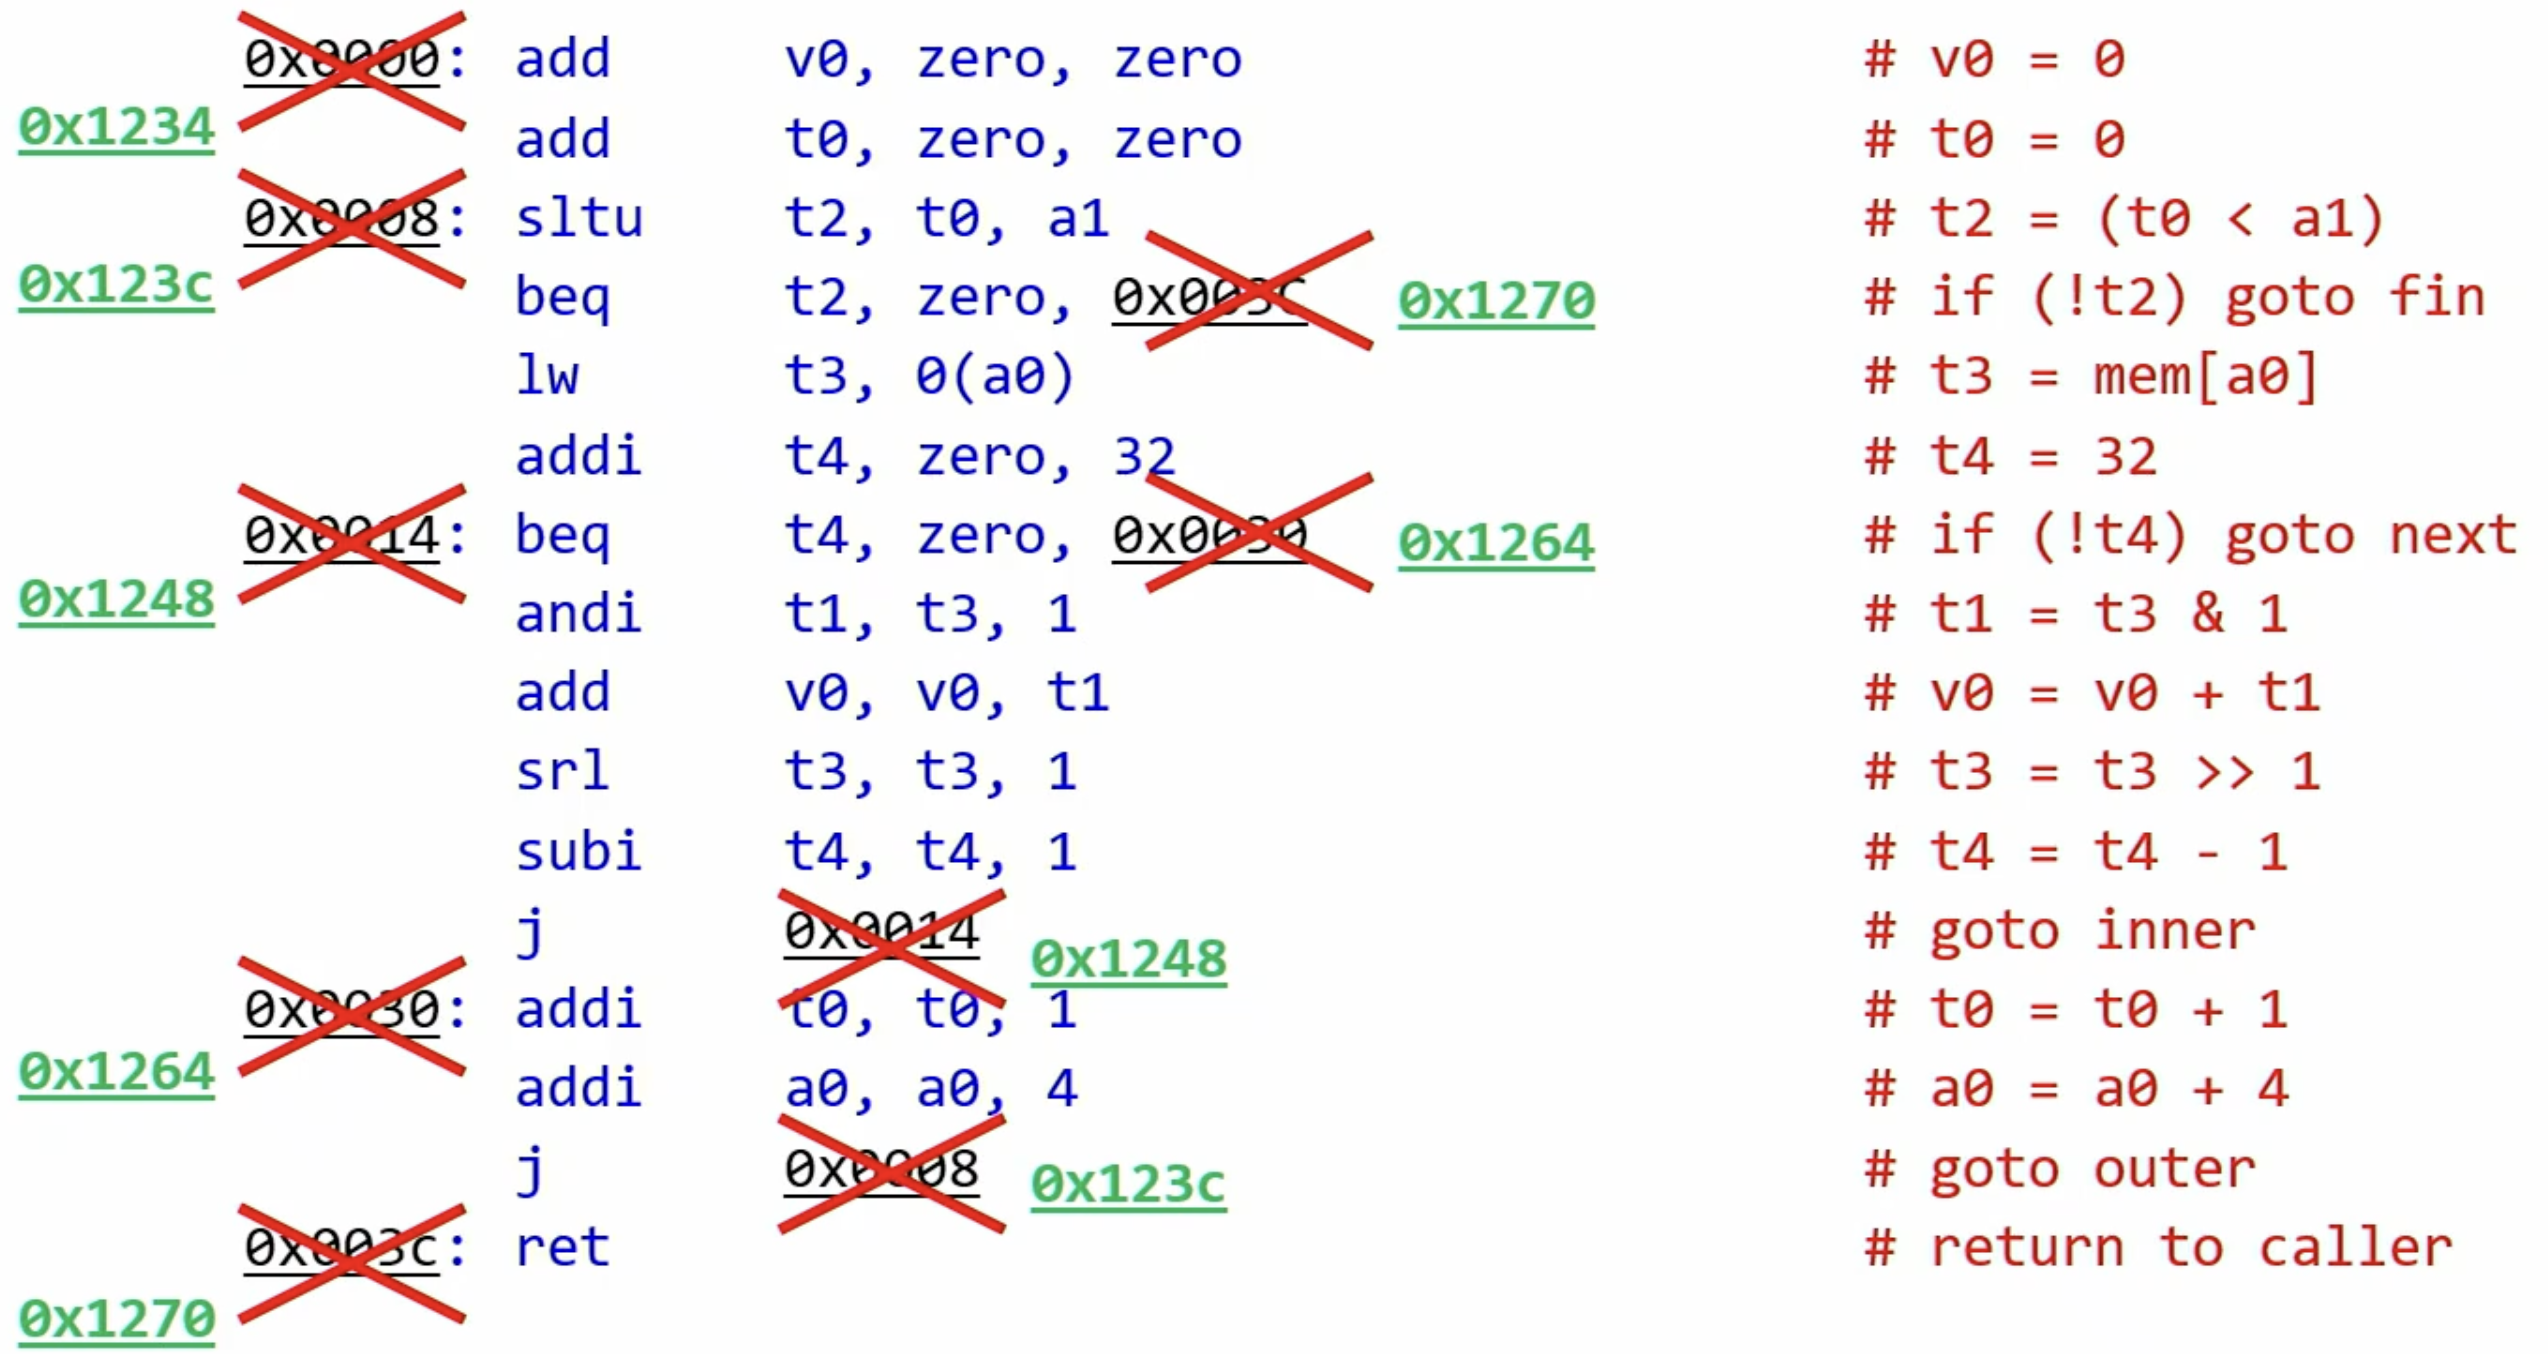
\includegraphics[width=0.65\textwidth]{chapters/chapter3c/images/relocate.png}
\end{center}

By performing these updates, the program adapts to the memory layout without requiring additional runtime computations. This process, though effective, operates primarily at the binary level rather than at the assembly code level.

\subsubsection{Binary-Level Adjustments}

Relocation at load time involves modifying the binary code directly. Specific fields within the machine instructions are updated based on relocation tables, which specify the exact memory addresses to be adjusted. These tables play a crucial role in streamlining the relocation process and ensuring correctness.
\begin{center}
    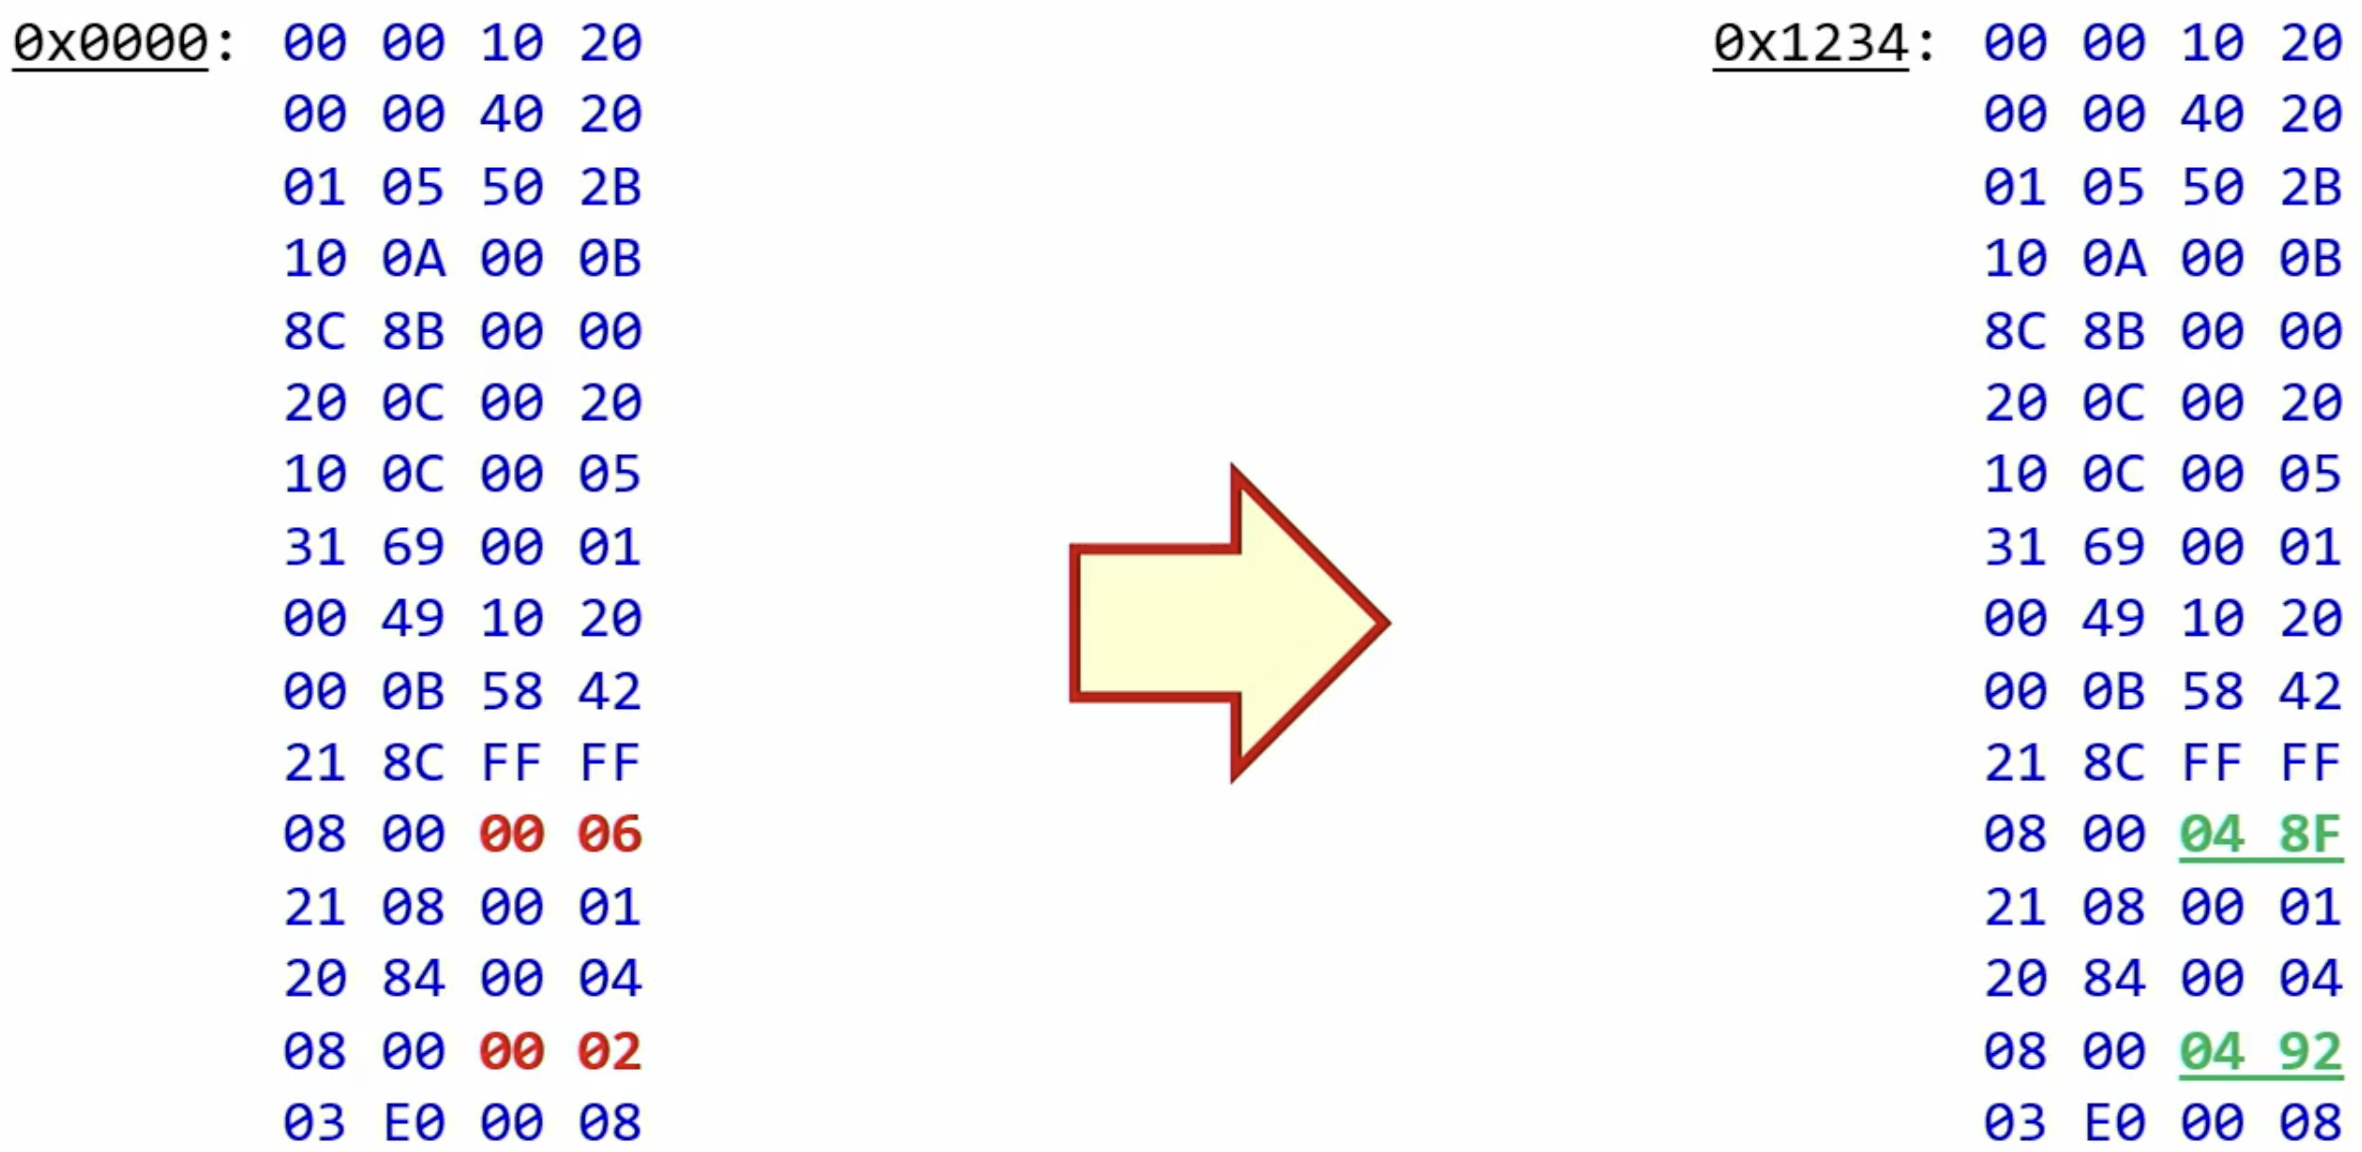
\includegraphics[width=0.65\textwidth]{chapters/chapter3c/images/relocate2.png}
\end{center}

For instance, consider a binary program initially loaded at a base address of \texttt{0x0000}. During relocation, placeholders in the binary instructions are replaced with actual memory addresses derived from the relocation table, as illustrated in the figure. This guarantees that memory references resolve correctly during execution.

\subsubsection{Memory Utilization and Limitations}

While relocation at load time simplifies memory address management, it is not without its drawbacks. As programs are loaded and terminated, gaps in memory may form, leading to inefficient utilization. This fragmentation becomes particularly problematic in systems with limited memory or dynamic memory allocation needs.
\begin{center}
    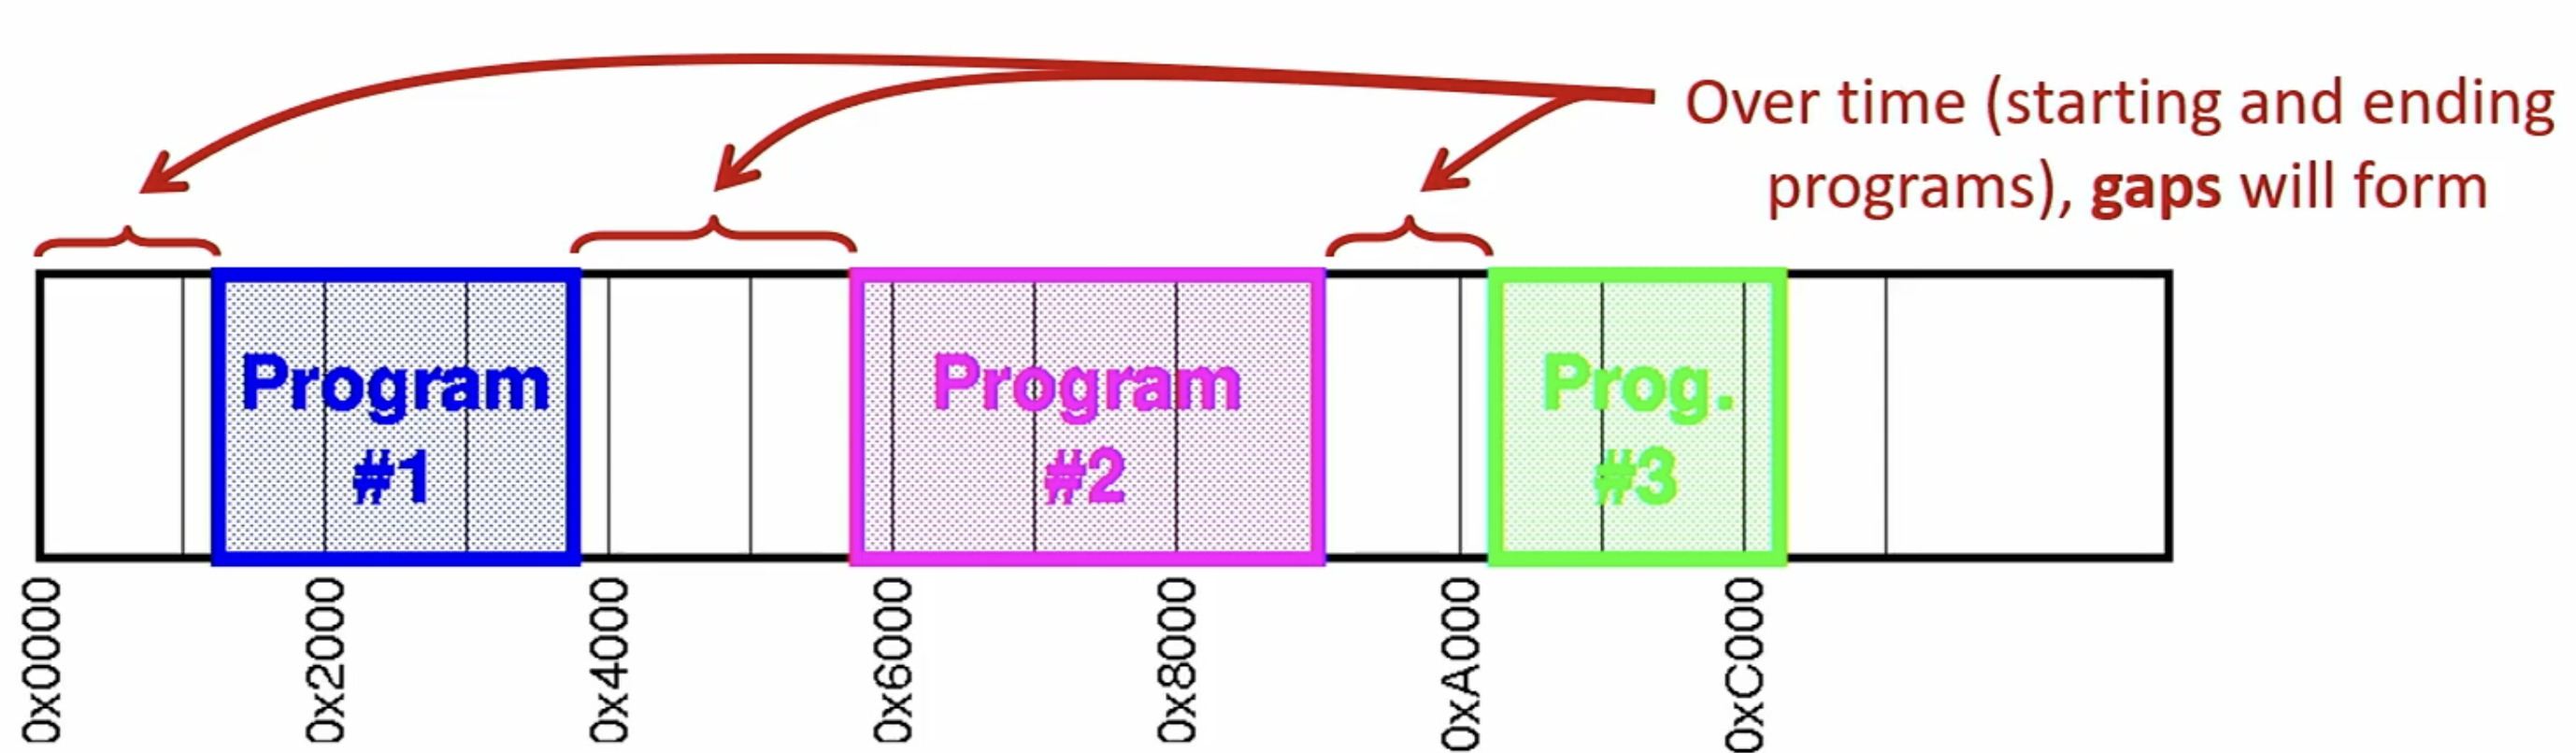
\includegraphics[width=0.65\textwidth]{chapters/chapter3c/images/relocate3.png}
\end{center}

\textbf{Limitations:}
\begin{itemize}
    \item \textit{High Overhead:} Relocation requires considerable computational effort at load time to allocate and adjust memory segments accurately.
    \item \textit{Inflexibility:} Once memory is allocated, it cannot be dynamically reconfigured, making it challenging to adapt to changing program requirements.
    \item \textit{Fragmentation Constraints:} Memory fragmentation caused by terminated programs can prevent loading a new program if its size exceeds the largest available gap, even when total free memory is sufficient (garbage collector\dots).
\end{itemize}
\subsection{Relocation in Hardware: Base and Bounds MMU}
Memory relocation is an essential process in modern computer systems to map virtual addresses to physical addresses. The \textbf{Base and Bounds Memory Management Unit (MMU)} facilitates this process dynamically by ensuring secure and efficient address translation.
\begin{center}
    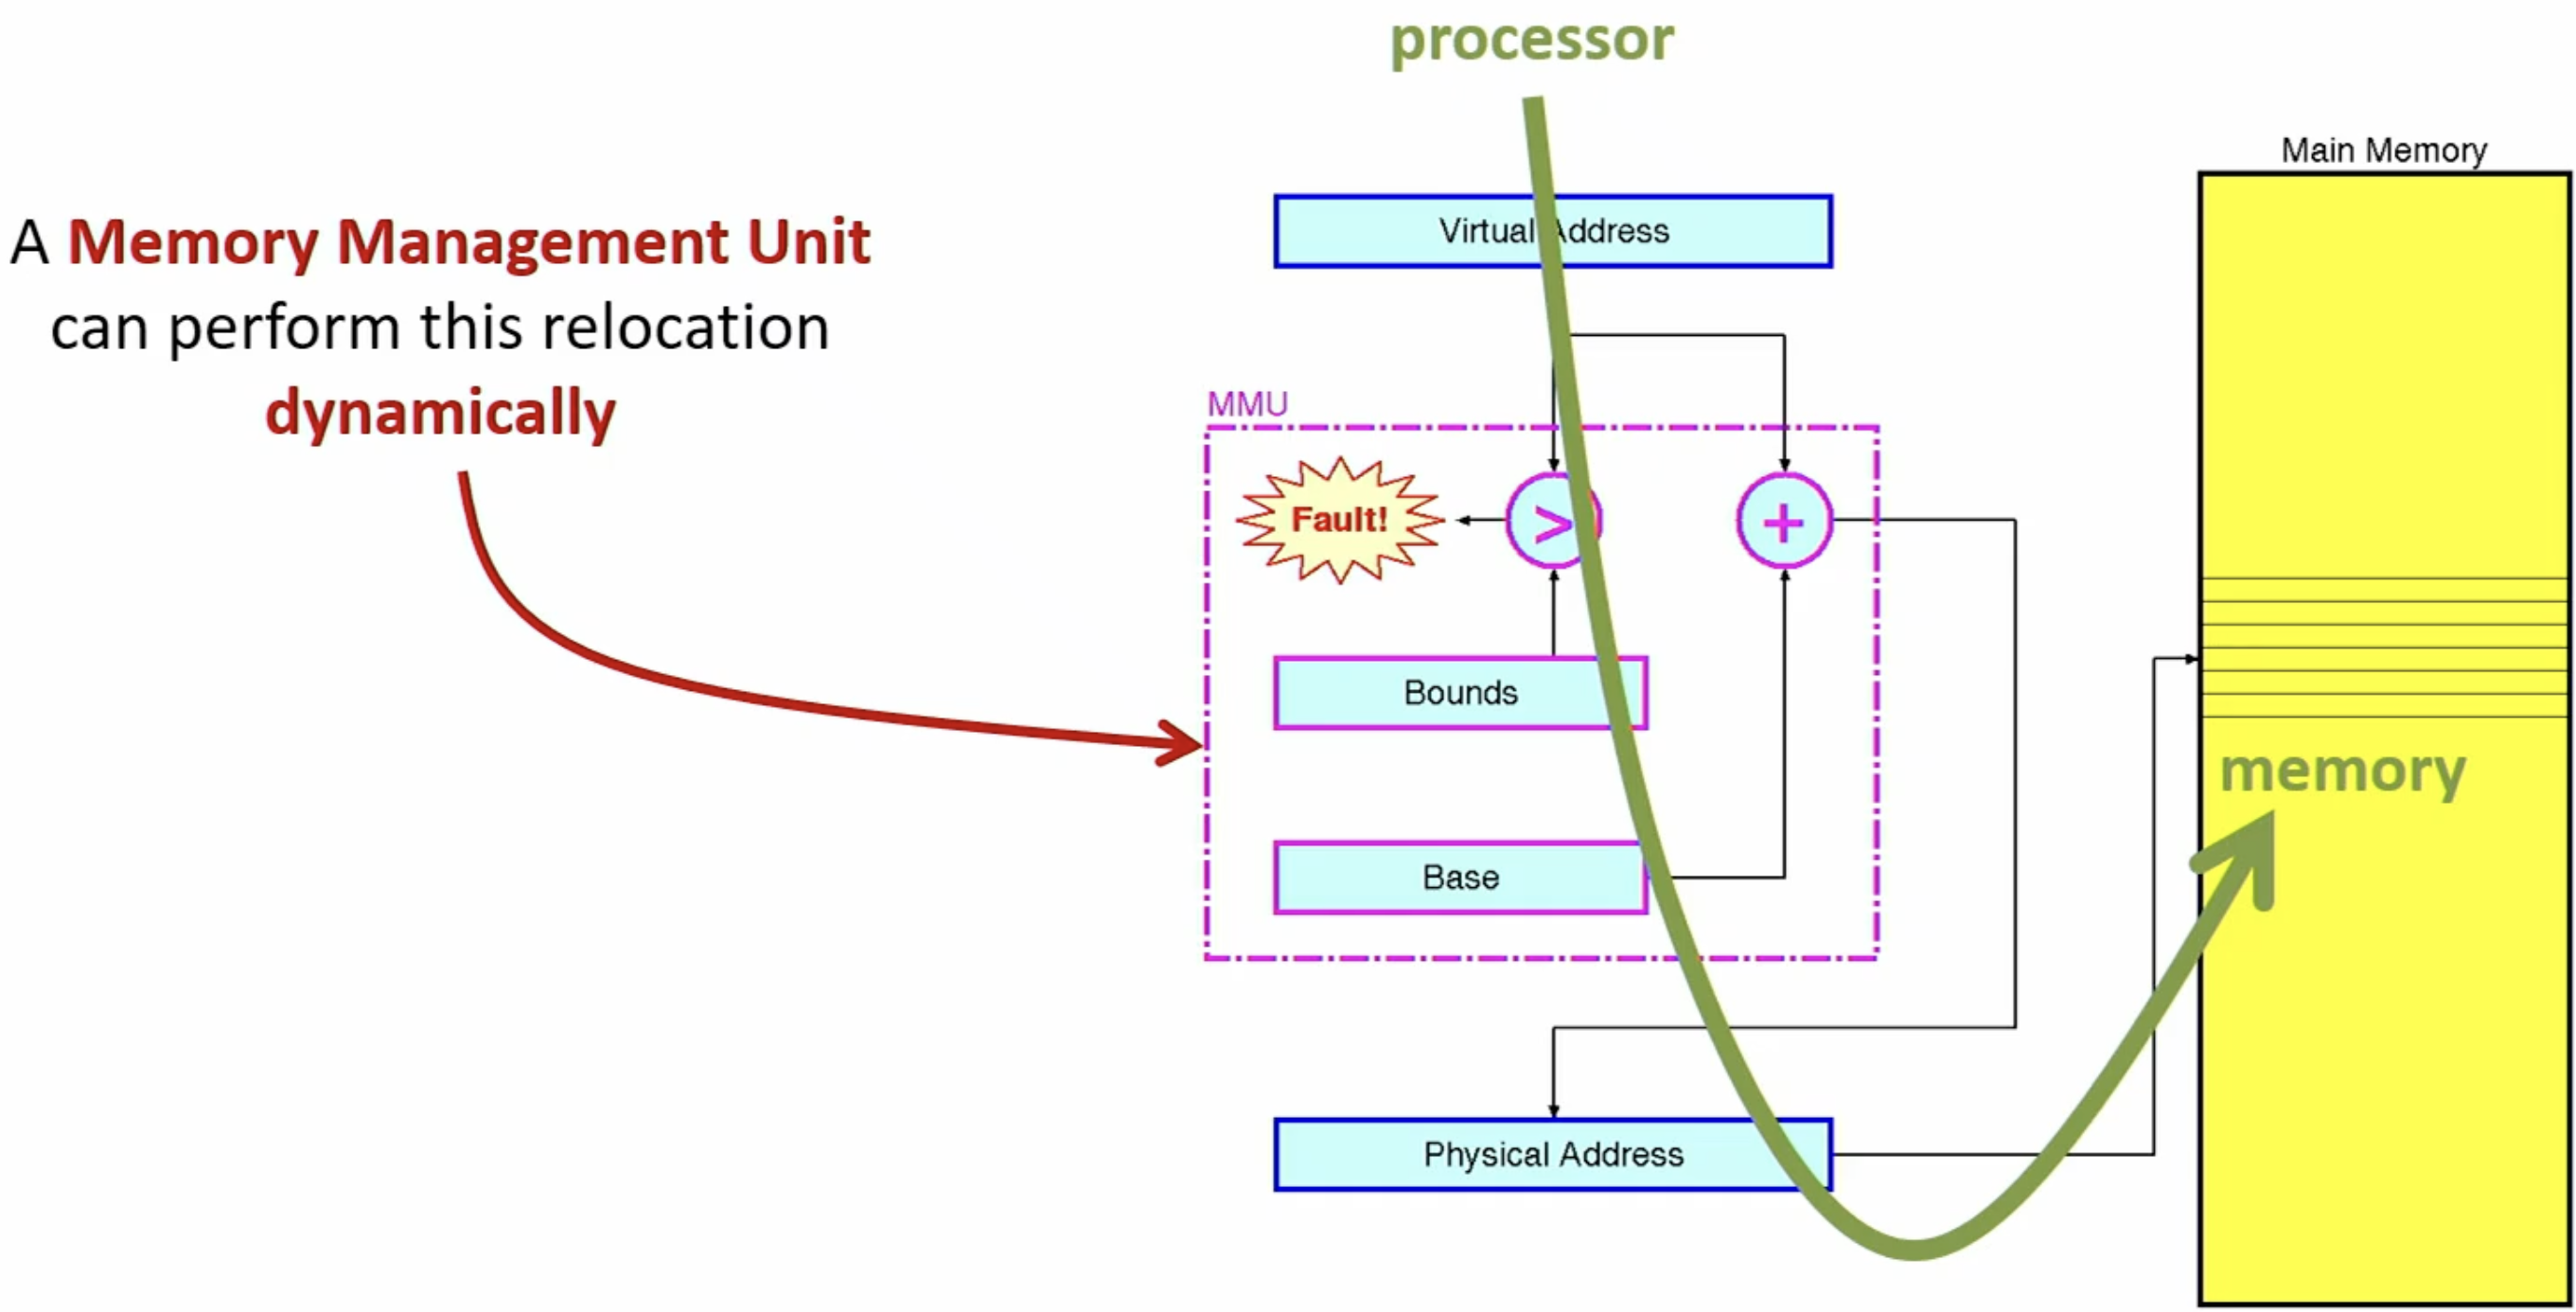
\includegraphics[width=0.65\textwidth]{chapters/chapter3c/images/MMU.png}
\end{center}
\begin{itemize}
    \item[-] \textbf{Base Register:} Holds the starting physical address of the process's memory.
    \item[-] \textbf{Bounds Register:} Defines the limit or size of the memory allocated to the process.
    \item[-] \textbf{Translation Process:}
    \begin{enumerate}
        \item The processor generates a \textit{virtual address}.
        \item The MMU checks if the virtual address exceeds the value in the \textit{Bounds Register}.
        \begin{itemize}
            \item If it exceeds, a \textbf{fault} is raised, preventing illegal memory access.
            \item Otherwise, the MMU adds the \textit{Base Register} value to the virtual address, producing the \textit{physical address}.
        \end{itemize}
        \item The \textit{physical address} is used to access the main memory.
    \end{enumerate}
\end{itemize}

This mechanism ensures process isolation and protects the system against unauthorized memory access, as only addresses within the defined bounds can be accessed. The dynamic nature of this relocation is key to supporting multitasking and efficient memory utilization.
\newpage
\subsection{Memory Management Unit (MMU)}
The \textbf{Memory Management Unit (MMU)} is a critical hardware component that facilitates the translation of \textit{virtual addresses} generated by the processor into \textit{physical addresses} used by the memory. This process is essential for efficient memory management in modern computer systems.

\begin{center}
    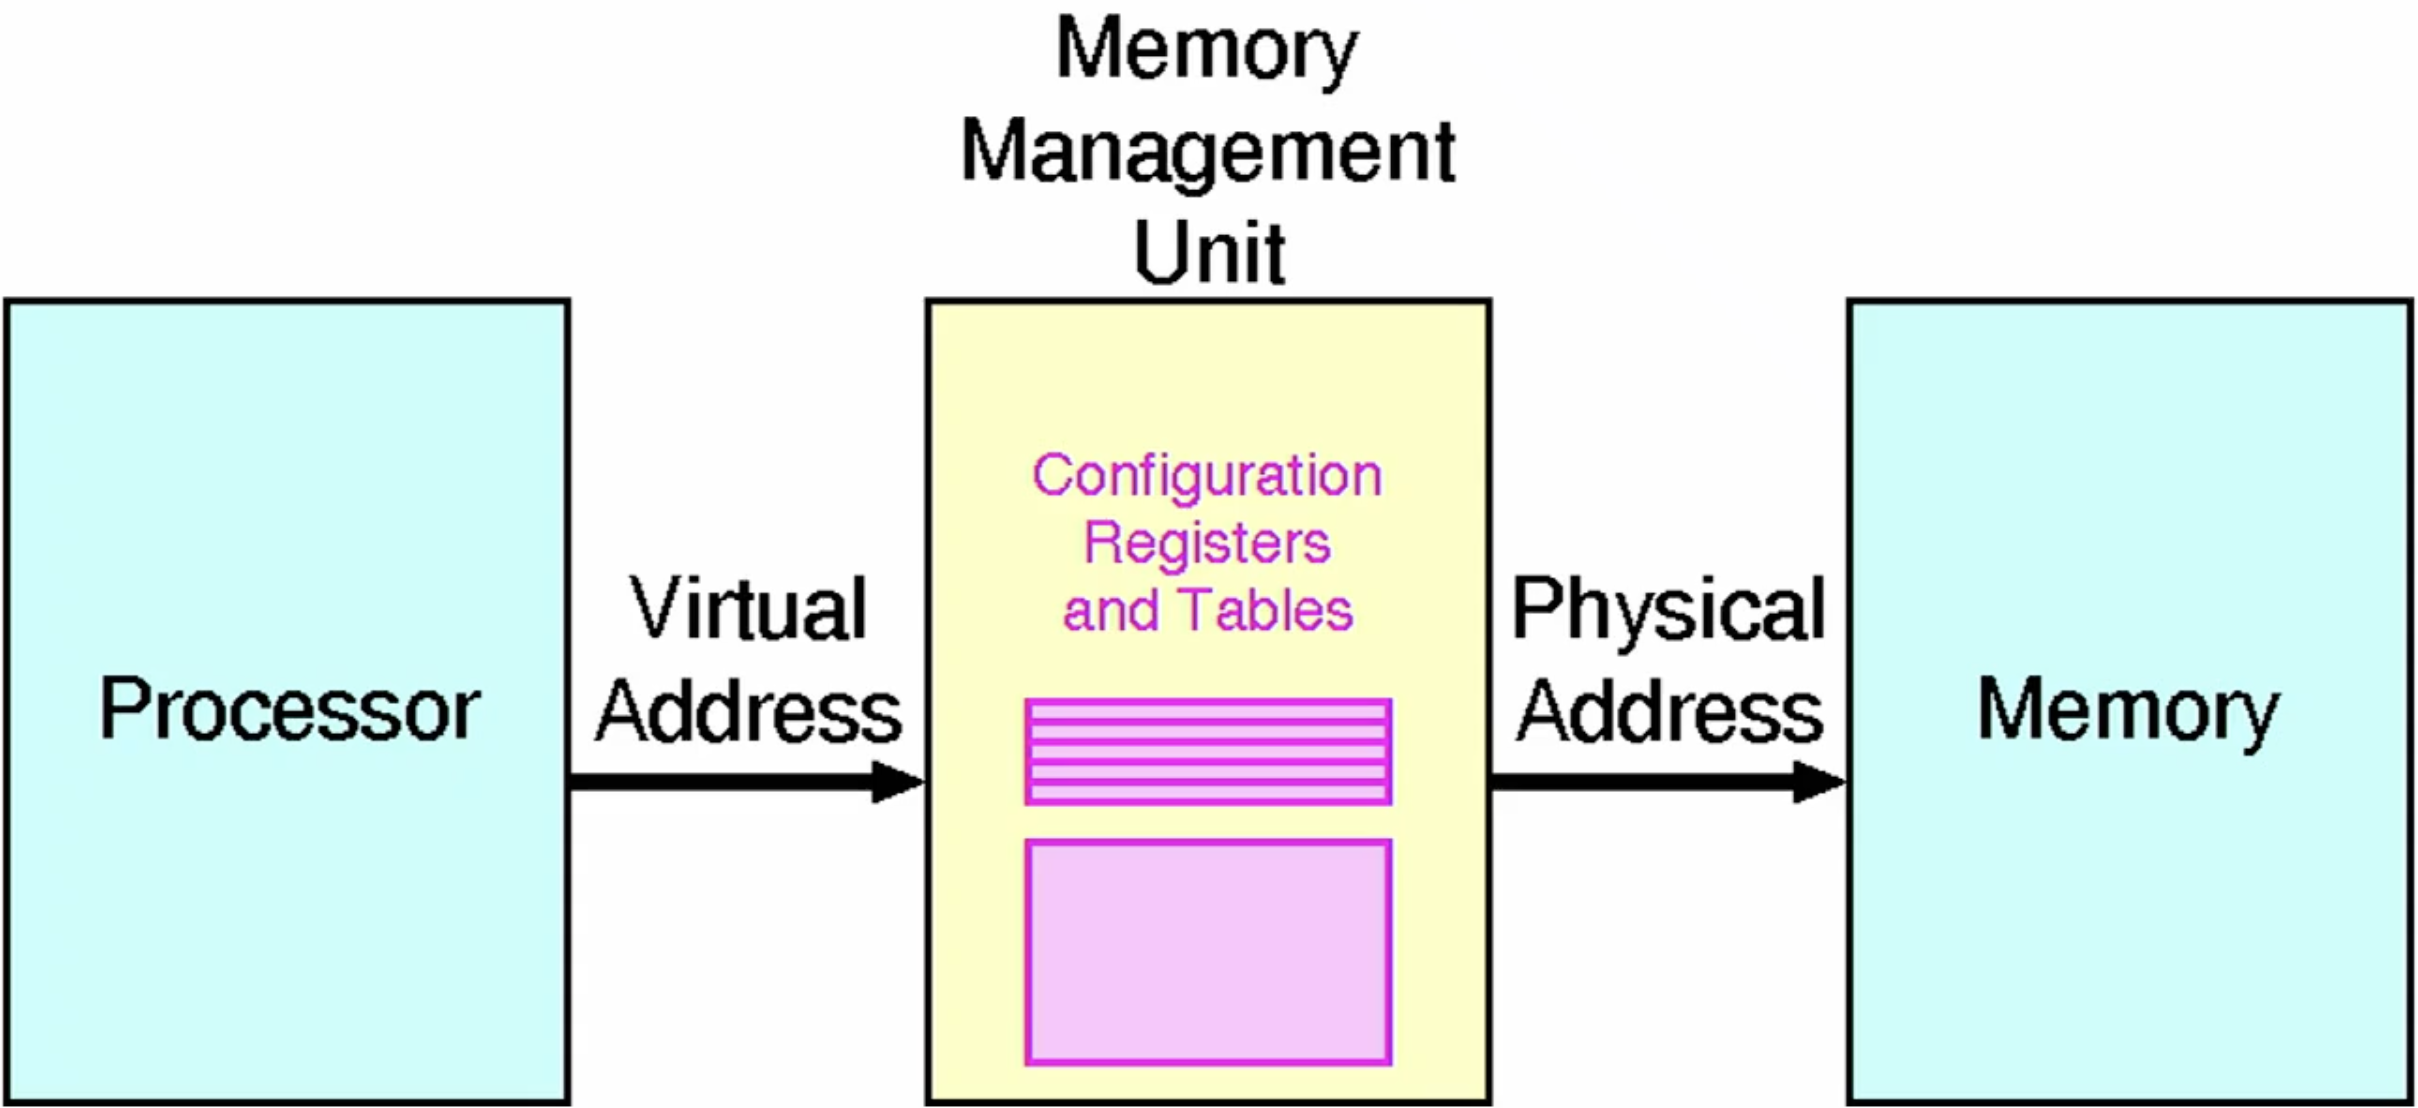
\includegraphics[width=0.65\textwidth]{chapters/chapter3c/images/MMU2.png}
\end{center}
\begin{itemize}
    \item[-] \textbf{Virtual Address:} Generated by the processor, representing a logical view of memory.
    \item[-] \textbf{Physical Address:} The actual address in the main memory where data is stored.
    \item[-] \textbf{Key Components:}
    \begin{enumerate}
        \item \textit{Configuration Registers:} Store information such as base addresses, bounds, and page tables.
        \item \textit{Translation Tables:} Facilitate the mapping of virtual to physical addresses.
    \end{enumerate}
    \item[-] \textbf{Process Overview:}
    \begin{enumerate}
        \item The processor generates a \textit{virtual address}.
        \item The MMU uses its configuration registers and translation tables to map the virtual address to a physical address.
        \item The mapped physical address is used to access data in the main memory.
    \end{enumerate}
\end{itemize}

\subsection{Program Relocation with Virtual Memory}
Virtual memory provides a powerful abstraction that decouples a program's logical memory view from the physical memory of the system. This flexibility is achieved by isolating programs from the underlying physical memory addresses, allowing dynamic relocation of programs without affecting their execution.
\begin{center}
    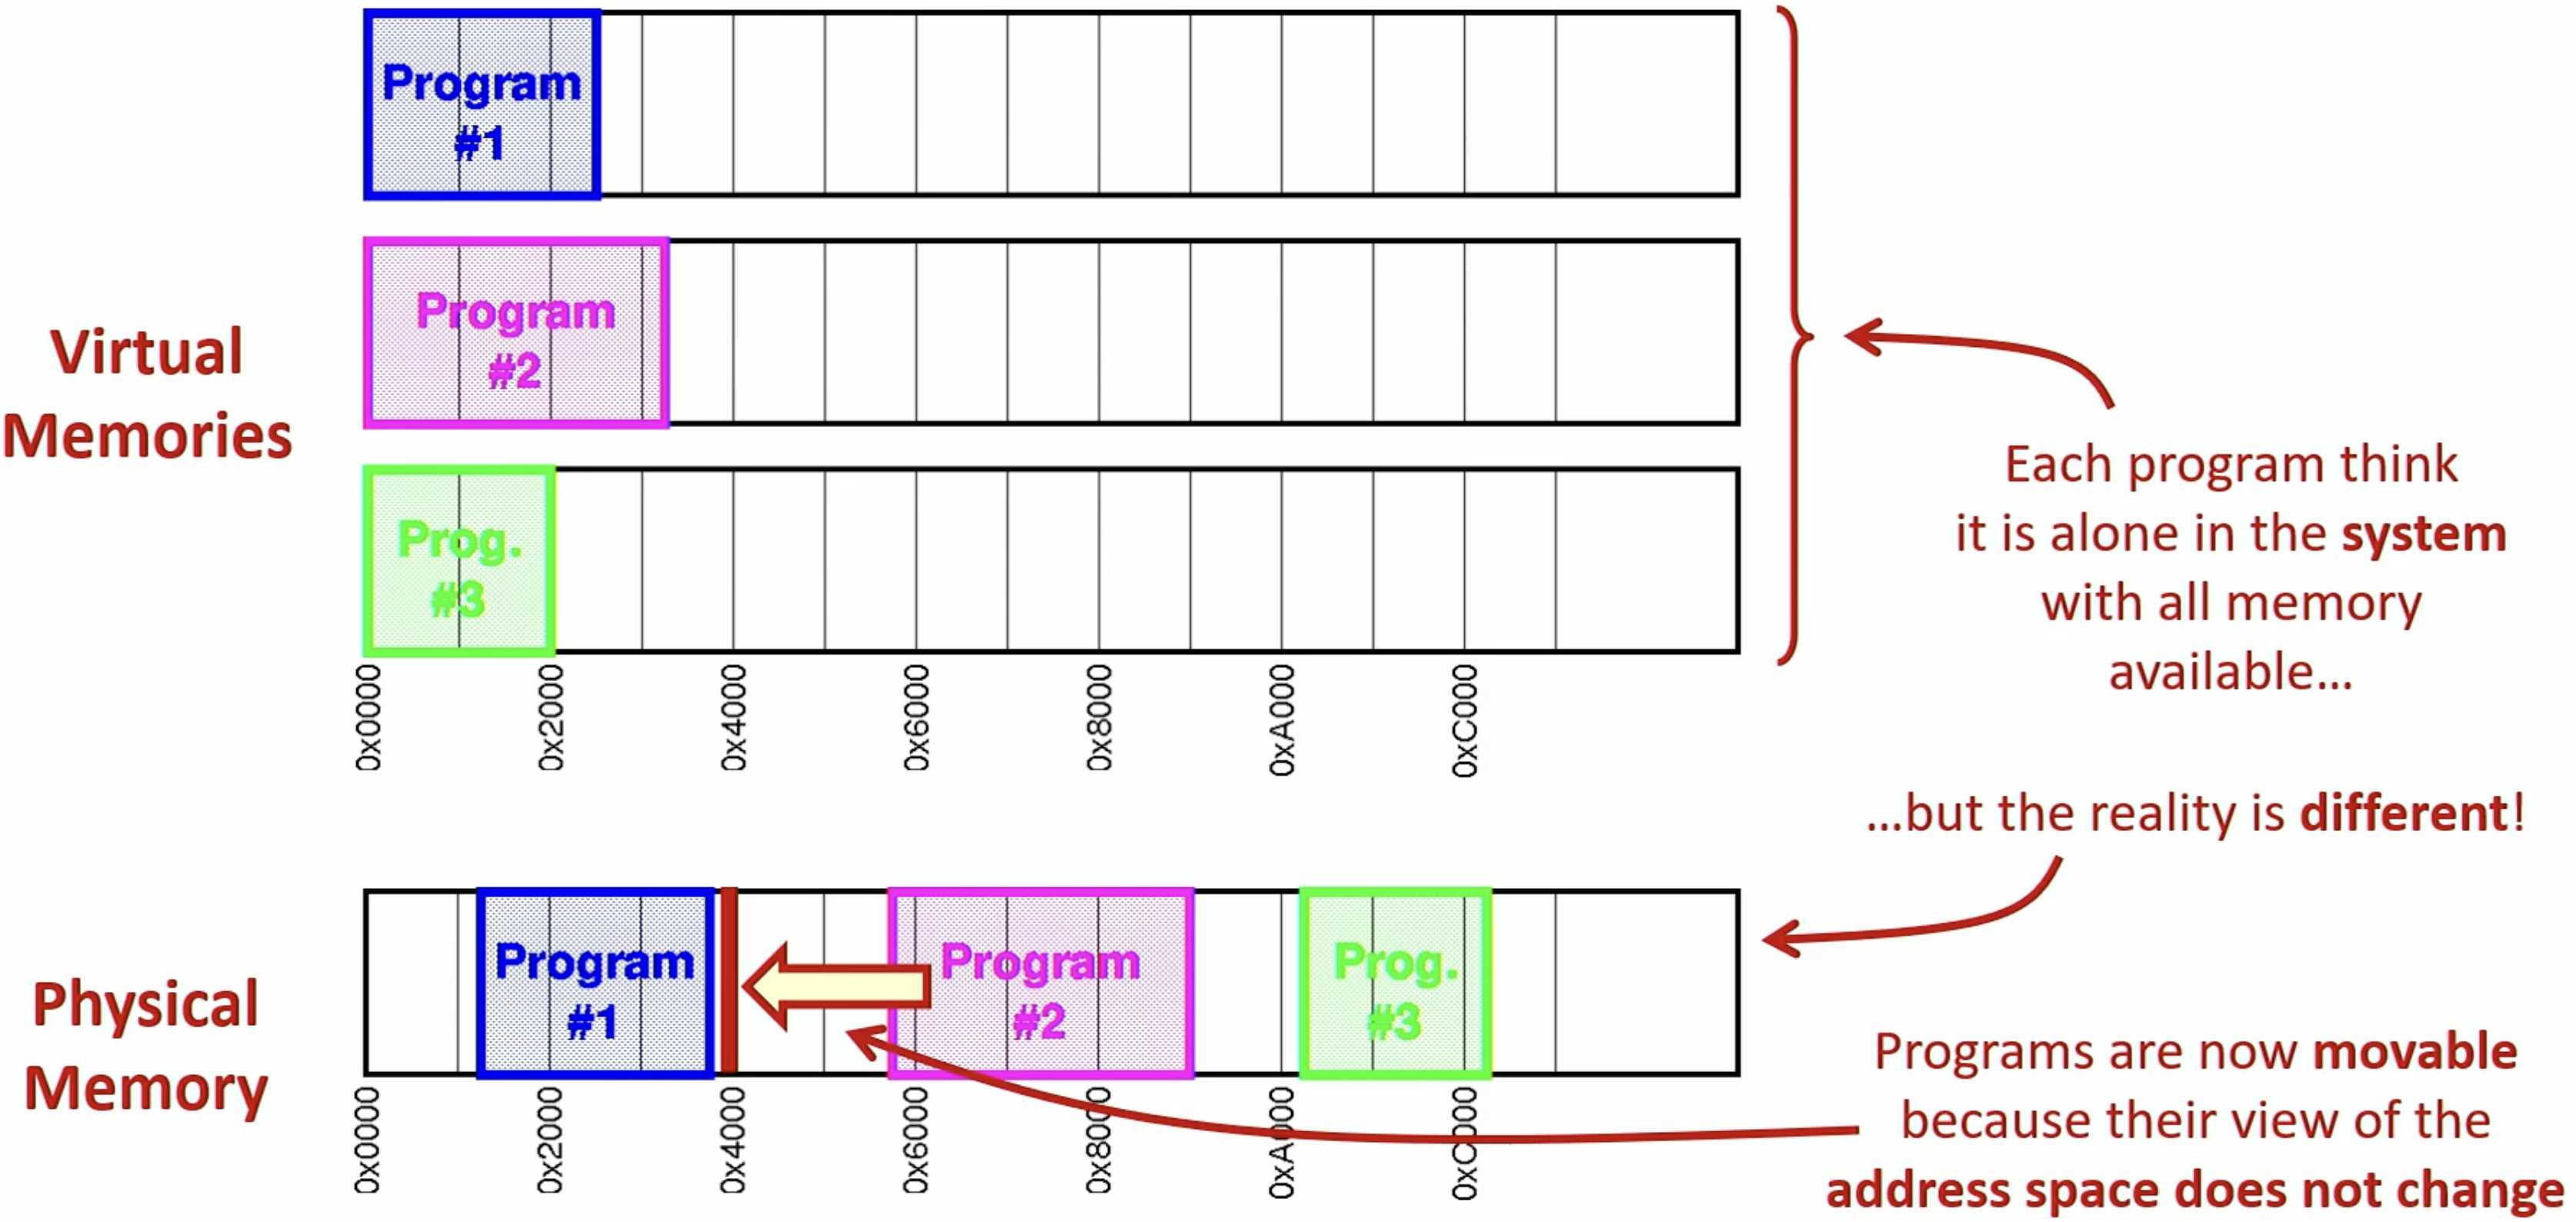
\includegraphics[width=0.65\textwidth]{chapters/chapter3c/images/virtual.png}
\end{center}
\begin{itemize}
    \item \textbf{Independent Address Spaces:} Each program is assigned its own virtual address space, creating the illusion that it has exclusive access to the entire memory. The program is unaware of its actual location in physical memory.
    \item \textbf{Program Relocation:} Since a program only interacts with its virtual address space, the operating system can freely move its physical location in memory as needed. This movement, known as \textit{relocation}, can occur during execution or at load time.
    \item \textbf{Benefits of Relocation:}
    \begin{itemize}
        \item \textit{Efficient Memory Use:} Programs can be compacted to free up contiguous physical memory for other processes.
        \item \textit{Load Balancing:} Active programs can be repositioned to optimize memory access speed or reduce fragmentation.
        \item \textit{Seamless Execution:} Since the memory translation is handled by the hardware (e.g., the Memory Management Unit, MMU), the program remains unaware of any changes in its physical location.
    \end{itemize}
\end{itemize}

\section{Relocation in Hardware: Base and Bounds MMU}
The Base and Bounds MMU (Memory Management Unit) is a hardware mechanism designed to facilitate memory relocation. It operates by performing two key actions on a virtual address provided by a process:
\begin{center}
    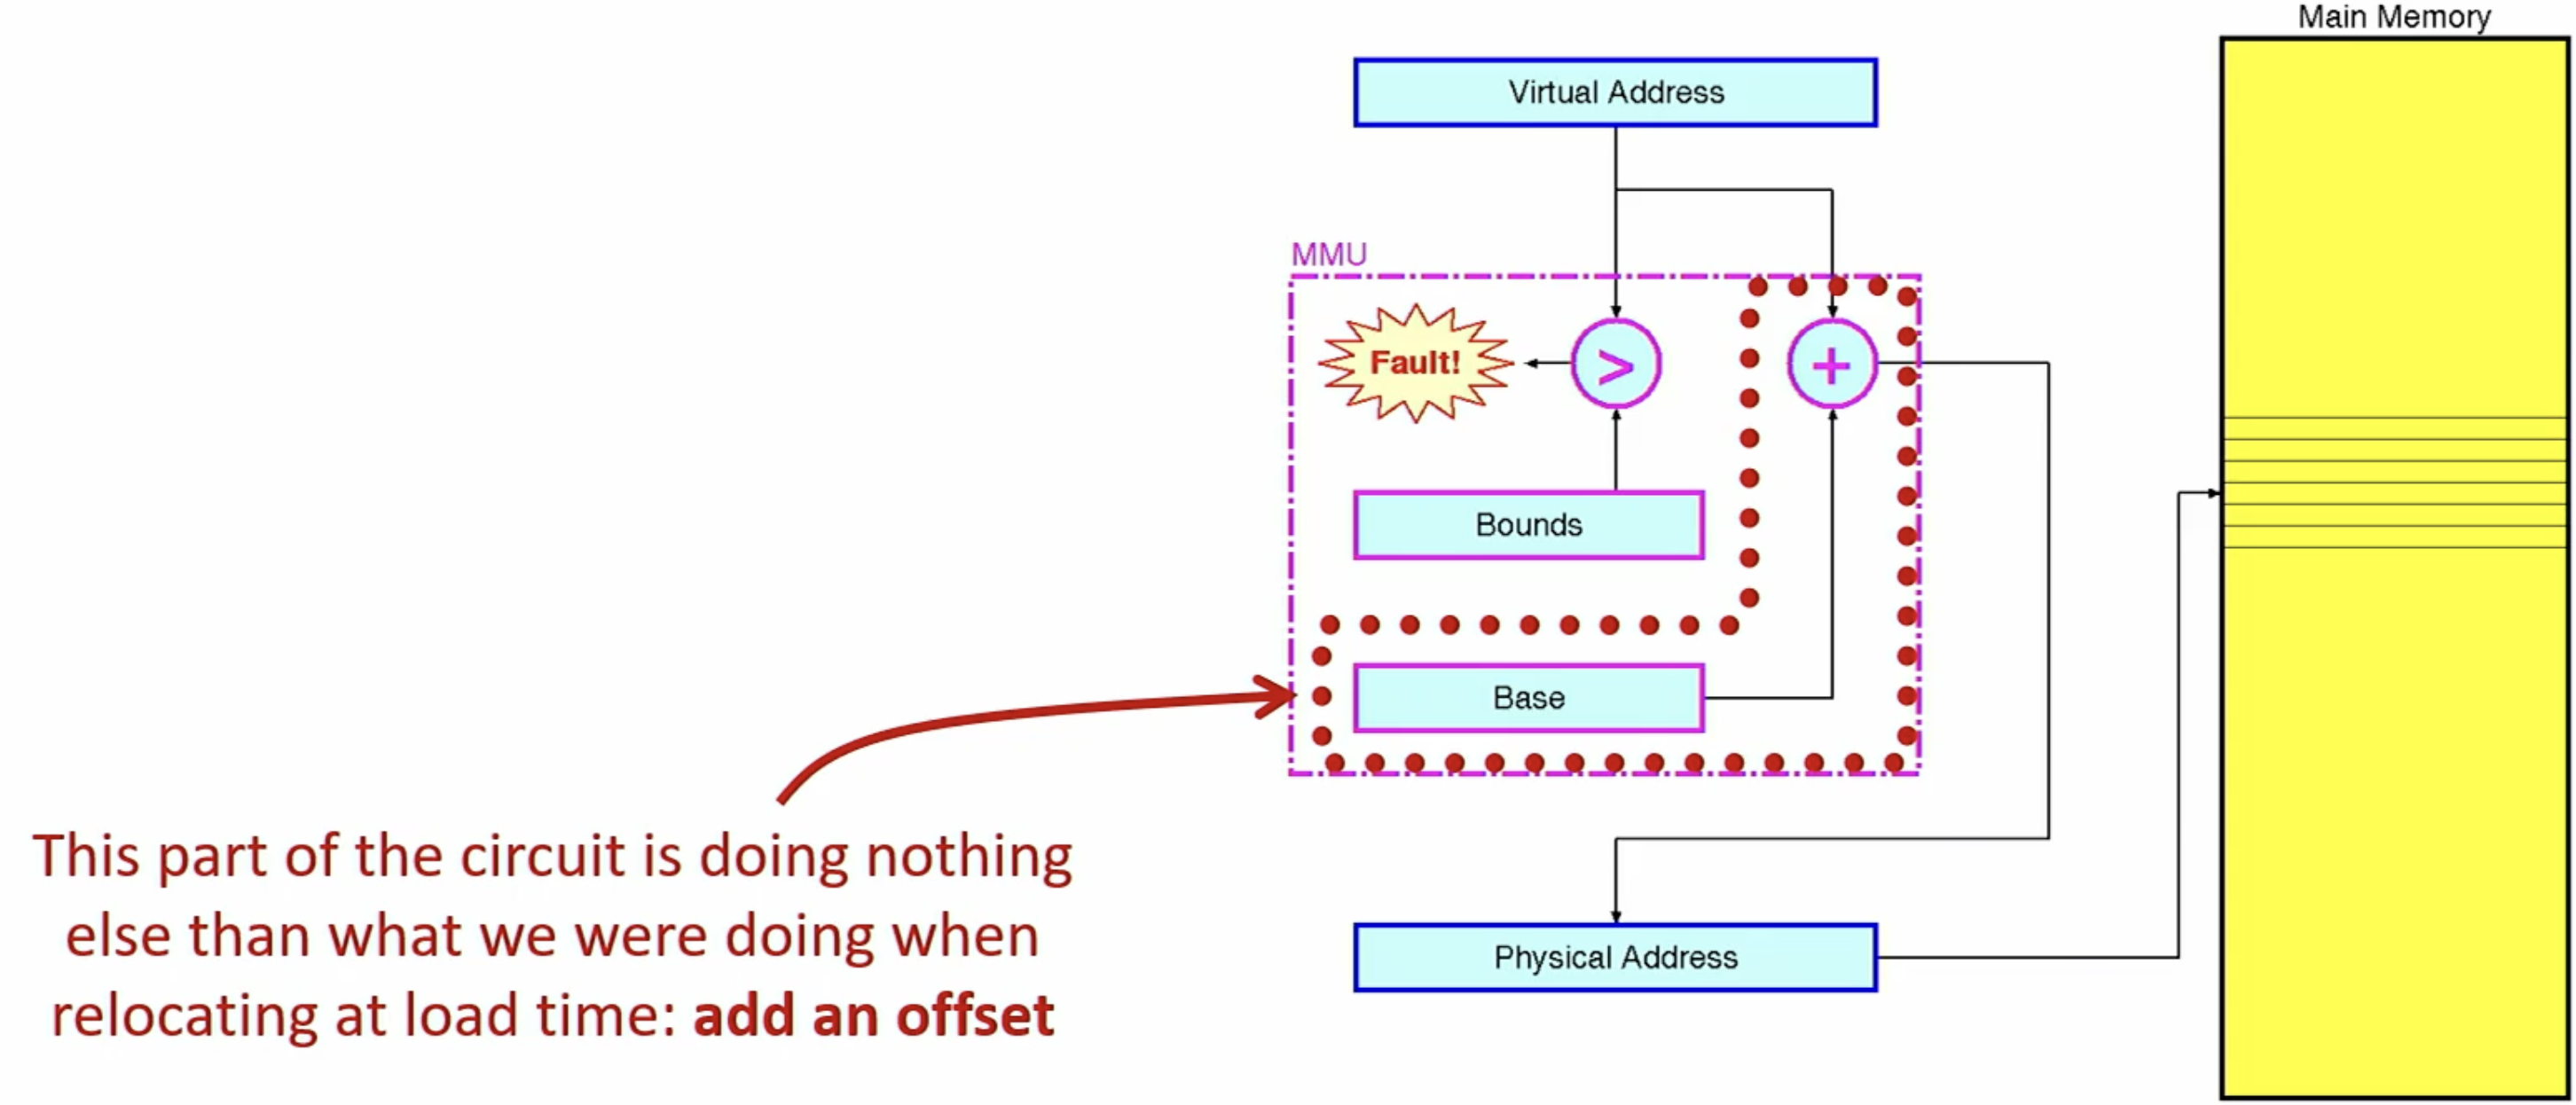
\includegraphics[width=0.65\textwidth]{chapters/chapter3c/images/relocation.png}
\end{center}
\begin{itemize}
    \item \textbf{Bounds Check:} The virtual address is compared with the \texttt{Bounds} register to ensure it is within the allowable range. If the virtual address exceeds the bounds, a fault is triggered, preventing unauthorized access.
    \item \textbf{Offset Addition:} If the virtual address is valid, it is added to the value in the \texttt{Base} register. This offset addition translates the virtual address into a physical address, which is then used to access the main memory.
\end{itemize}

\subsection{Preventing Overreach in Virtual and Physical Memory}
In systems using virtual memory, it is critical to ensure that programs remain within their allocated address spaces. If a program accesses memory beyond its assigned virtual boundaries, it risks overlapping with another program's memory. This can lead to severe security and stability issues.
\begin{center}
    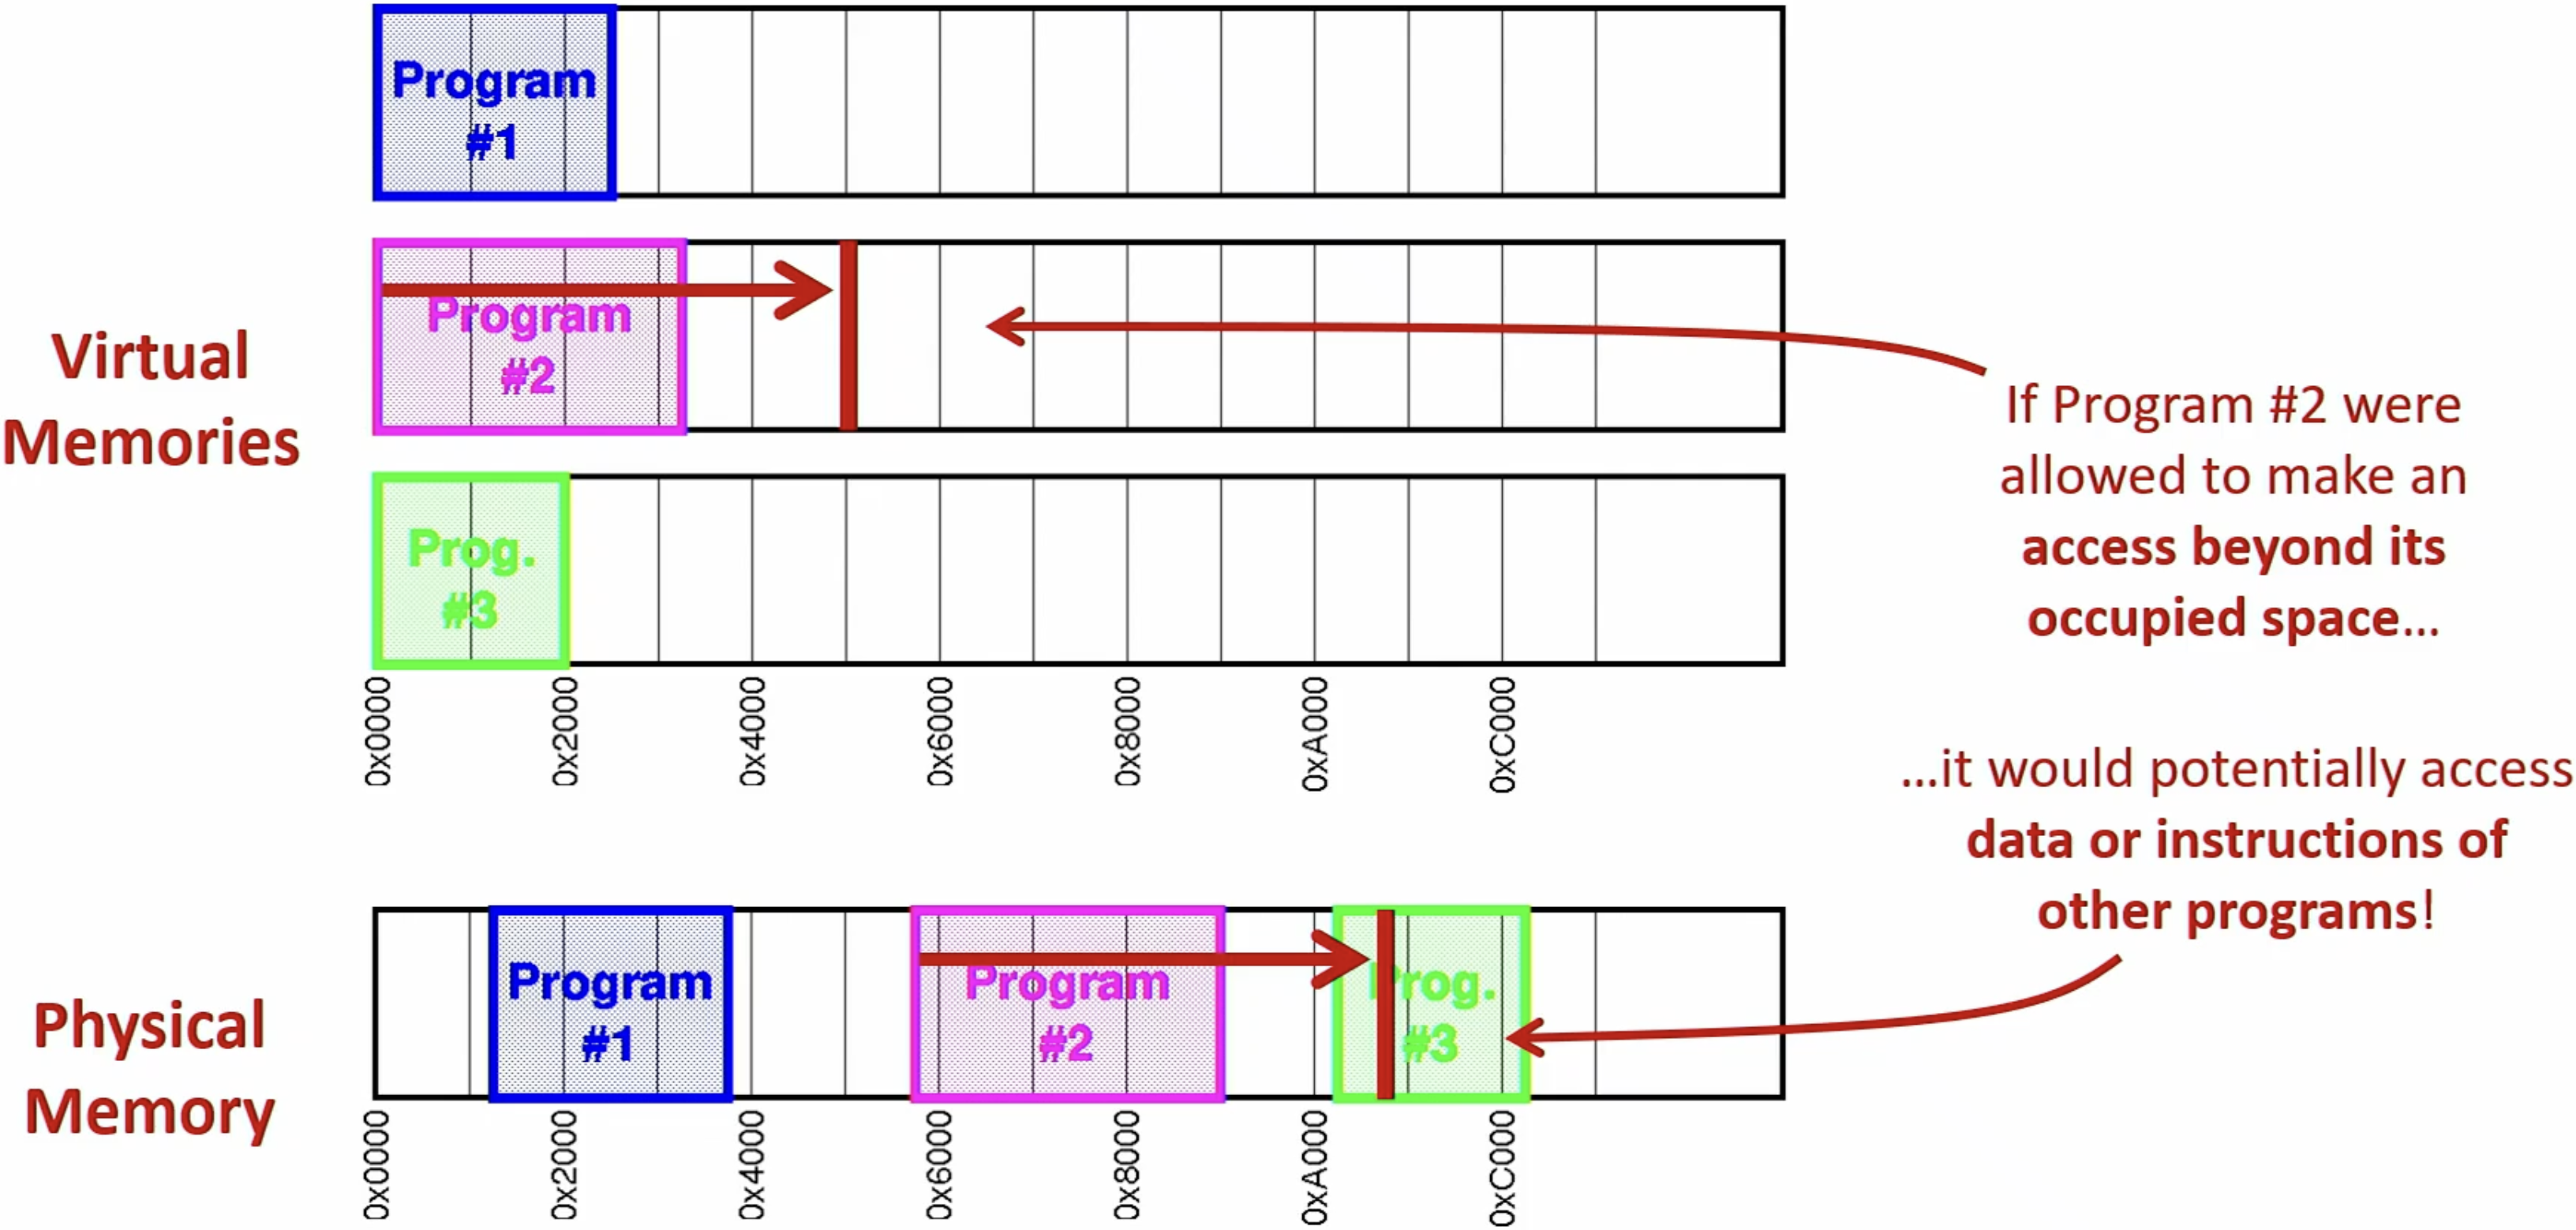
\includegraphics[width=0.65\textwidth]{chapters/chapter3c/images/fault.png}
\end{center}
\begin{itemize}
    \item[-] \textbf{Virtual Memory Overreach:} Each program is given its own virtual address space. However, if a program attempts to access an address outside its bounds, it could inadvertently access data or instructions from another program. This can compromise the integrity of both programs.
    \item[-] \textbf{MMU Checks:} To prevent such overreach, the Memory Management Unit (MMU) enforces strict bounds checking. It ensures that all memory accesses fall within the allowed range defined by the program's base and bounds registers. If a memory access is outside these bounds, the MMU generates a fault, preventing the access.
    \item[-] \textbf{Physical Memory Isolation:} Even though programs use virtual addresses, these are translated to physical addresses by the MMU. Proper isolation ensures that physical memory regions assigned to different programs do not overlap, maintaining system stability.
\end{itemize}

This mechanism of bounds checking and fault generation safeguards against unintended interactions between programs and ensures that no program can overwrite or access another program's data.

\subsection{Base and Bounds MMU}

\begin{center} 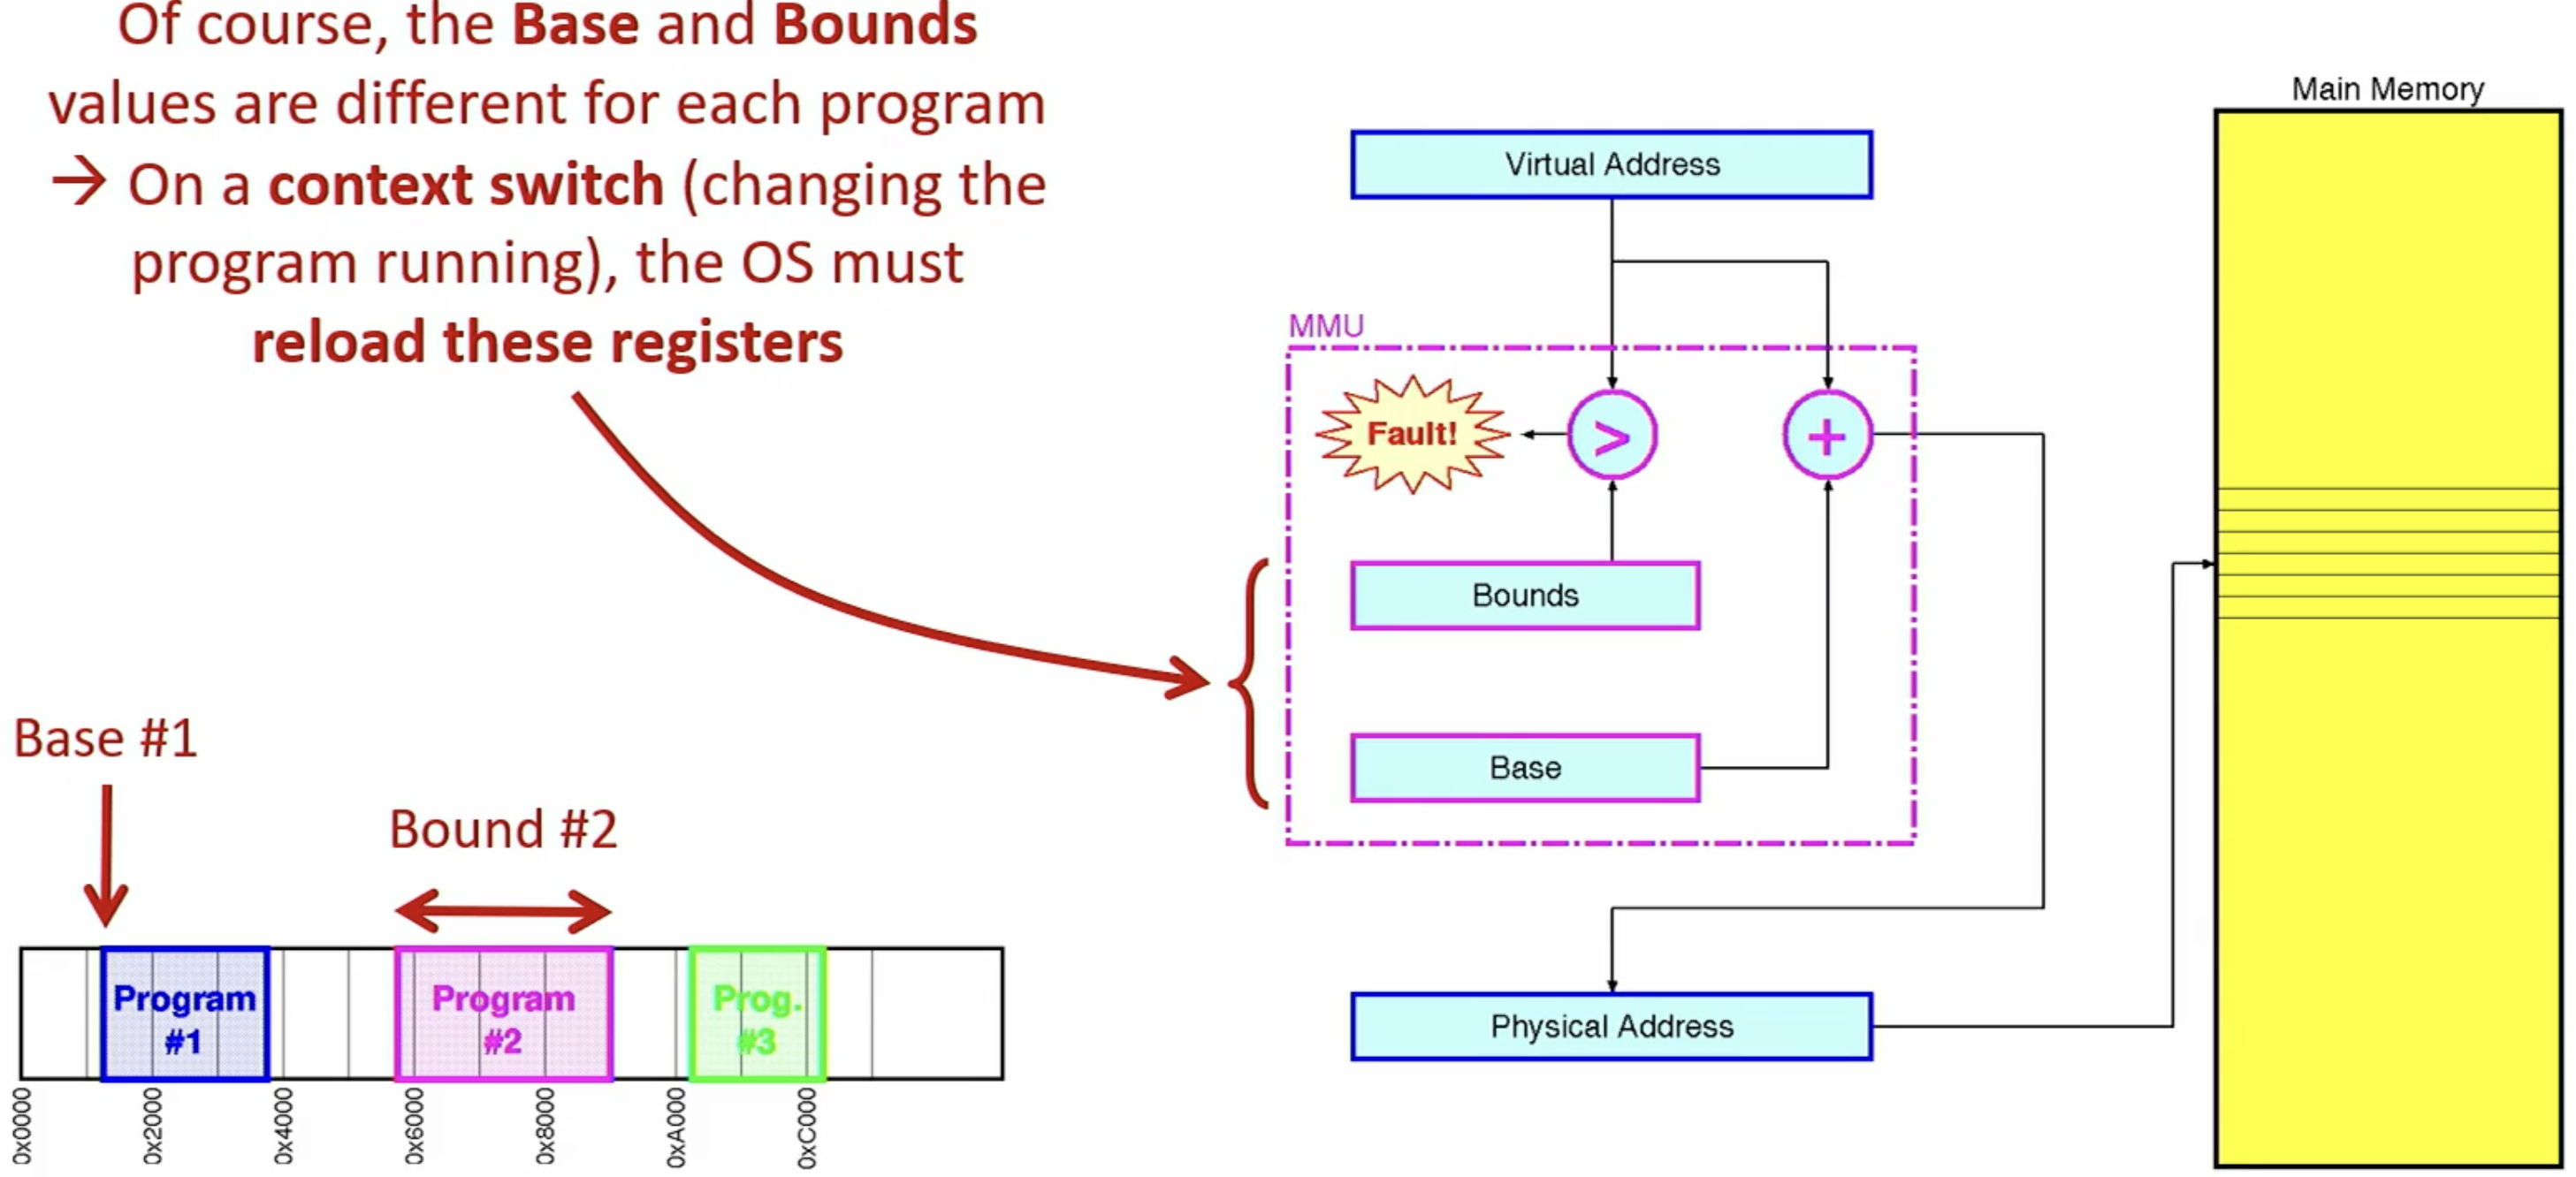
\includegraphics[width=0.65\textwidth]{chapters/chapter3c/images/bb.png} \end{center}

The Base and Bounds mechanism in the MMU defines the memory allocation for a process as follows:

\begin{itemize} \item Base: The starting address of the process's allocated memory. \item Bounds: The upper limit or size of the memory allocated to the process. \end{itemize}

\section{Needs of a Multiprogrammed System}

Multiprogrammed systems require efficient handling of memory and process management to ensure reliability and performance. The key requirements are as follows:

\begin{itemize}
    \item[-] \textbf{Relocation:} Programs must be written without prior knowledge of their location in memory. This ensures flexibility when allocating memory during execution.

    \item[-] \textbf{Protection:} Programs are restricted to access only their own data, safeguarding against interference from other programs. However, this protection mechanism can sometimes be crude, as it often limits each program to a single chunk of memory.

    \item[-] \textbf{Space Management:} When several programs run simultaneously, memory shortages may arise. Effective space allocation strategies are needed, which may involve techniques such as garbage collection and moving programs or data to optimize memory usage.
\end{itemize}

\section{Segmentation and Paging}
\begin{center}
    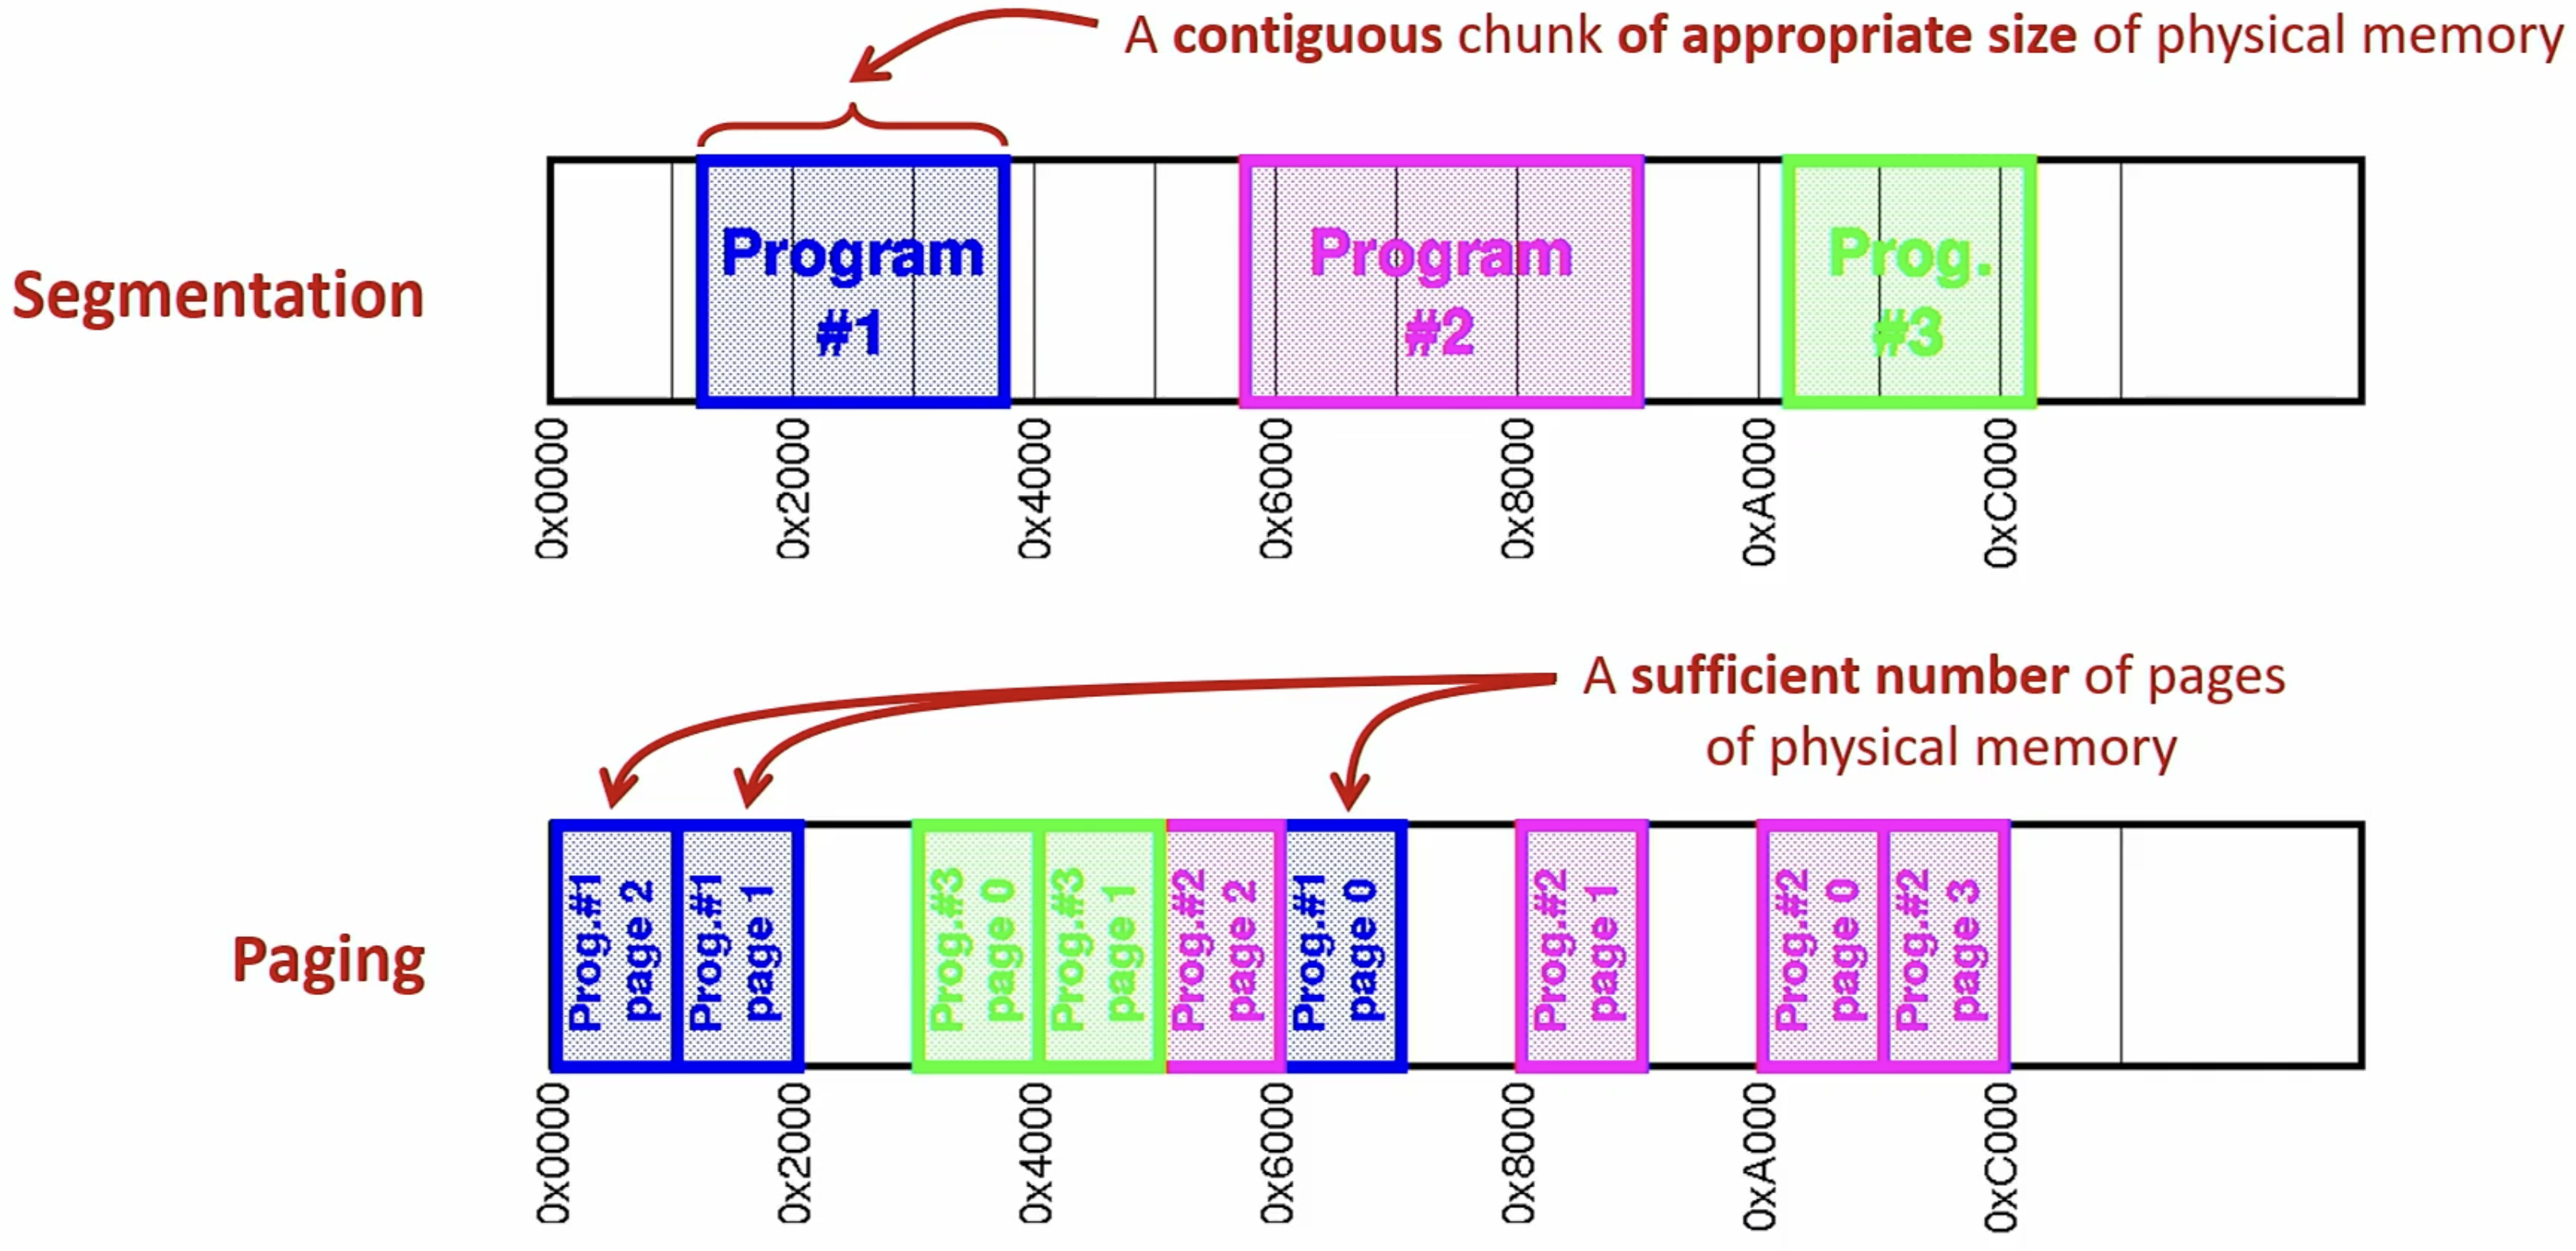
\includegraphics[width=0.65\textwidth]{chapters/chapter3c/images/segPage.png}
\end{center}
\paragraph{Segmentation:} Segmentation, an extension of the Base and Bounds technique, allows memory to be split exactly as needed by each program. Key characteristics include:
\begin{itemize}
    \item[-] Arbitrary starting point of a memory block.
    \item[-] Arbitrary length of memory blocks.
    \item[-] Multiple blocks can be allocated per application.
\end{itemize}

\paragraph{Paging:} Paging divides memory into equal-sized small blocks (e.g., 4–64~KiB) and assigns as many blocks as required to each program. This ensures uniformity in memory allocation.

\subsection{How do we Translate Now?}
Now we need to translate virtual addresses to physical addresses (with our new paging constraints). This process involves the following steps:
\begin{center}
    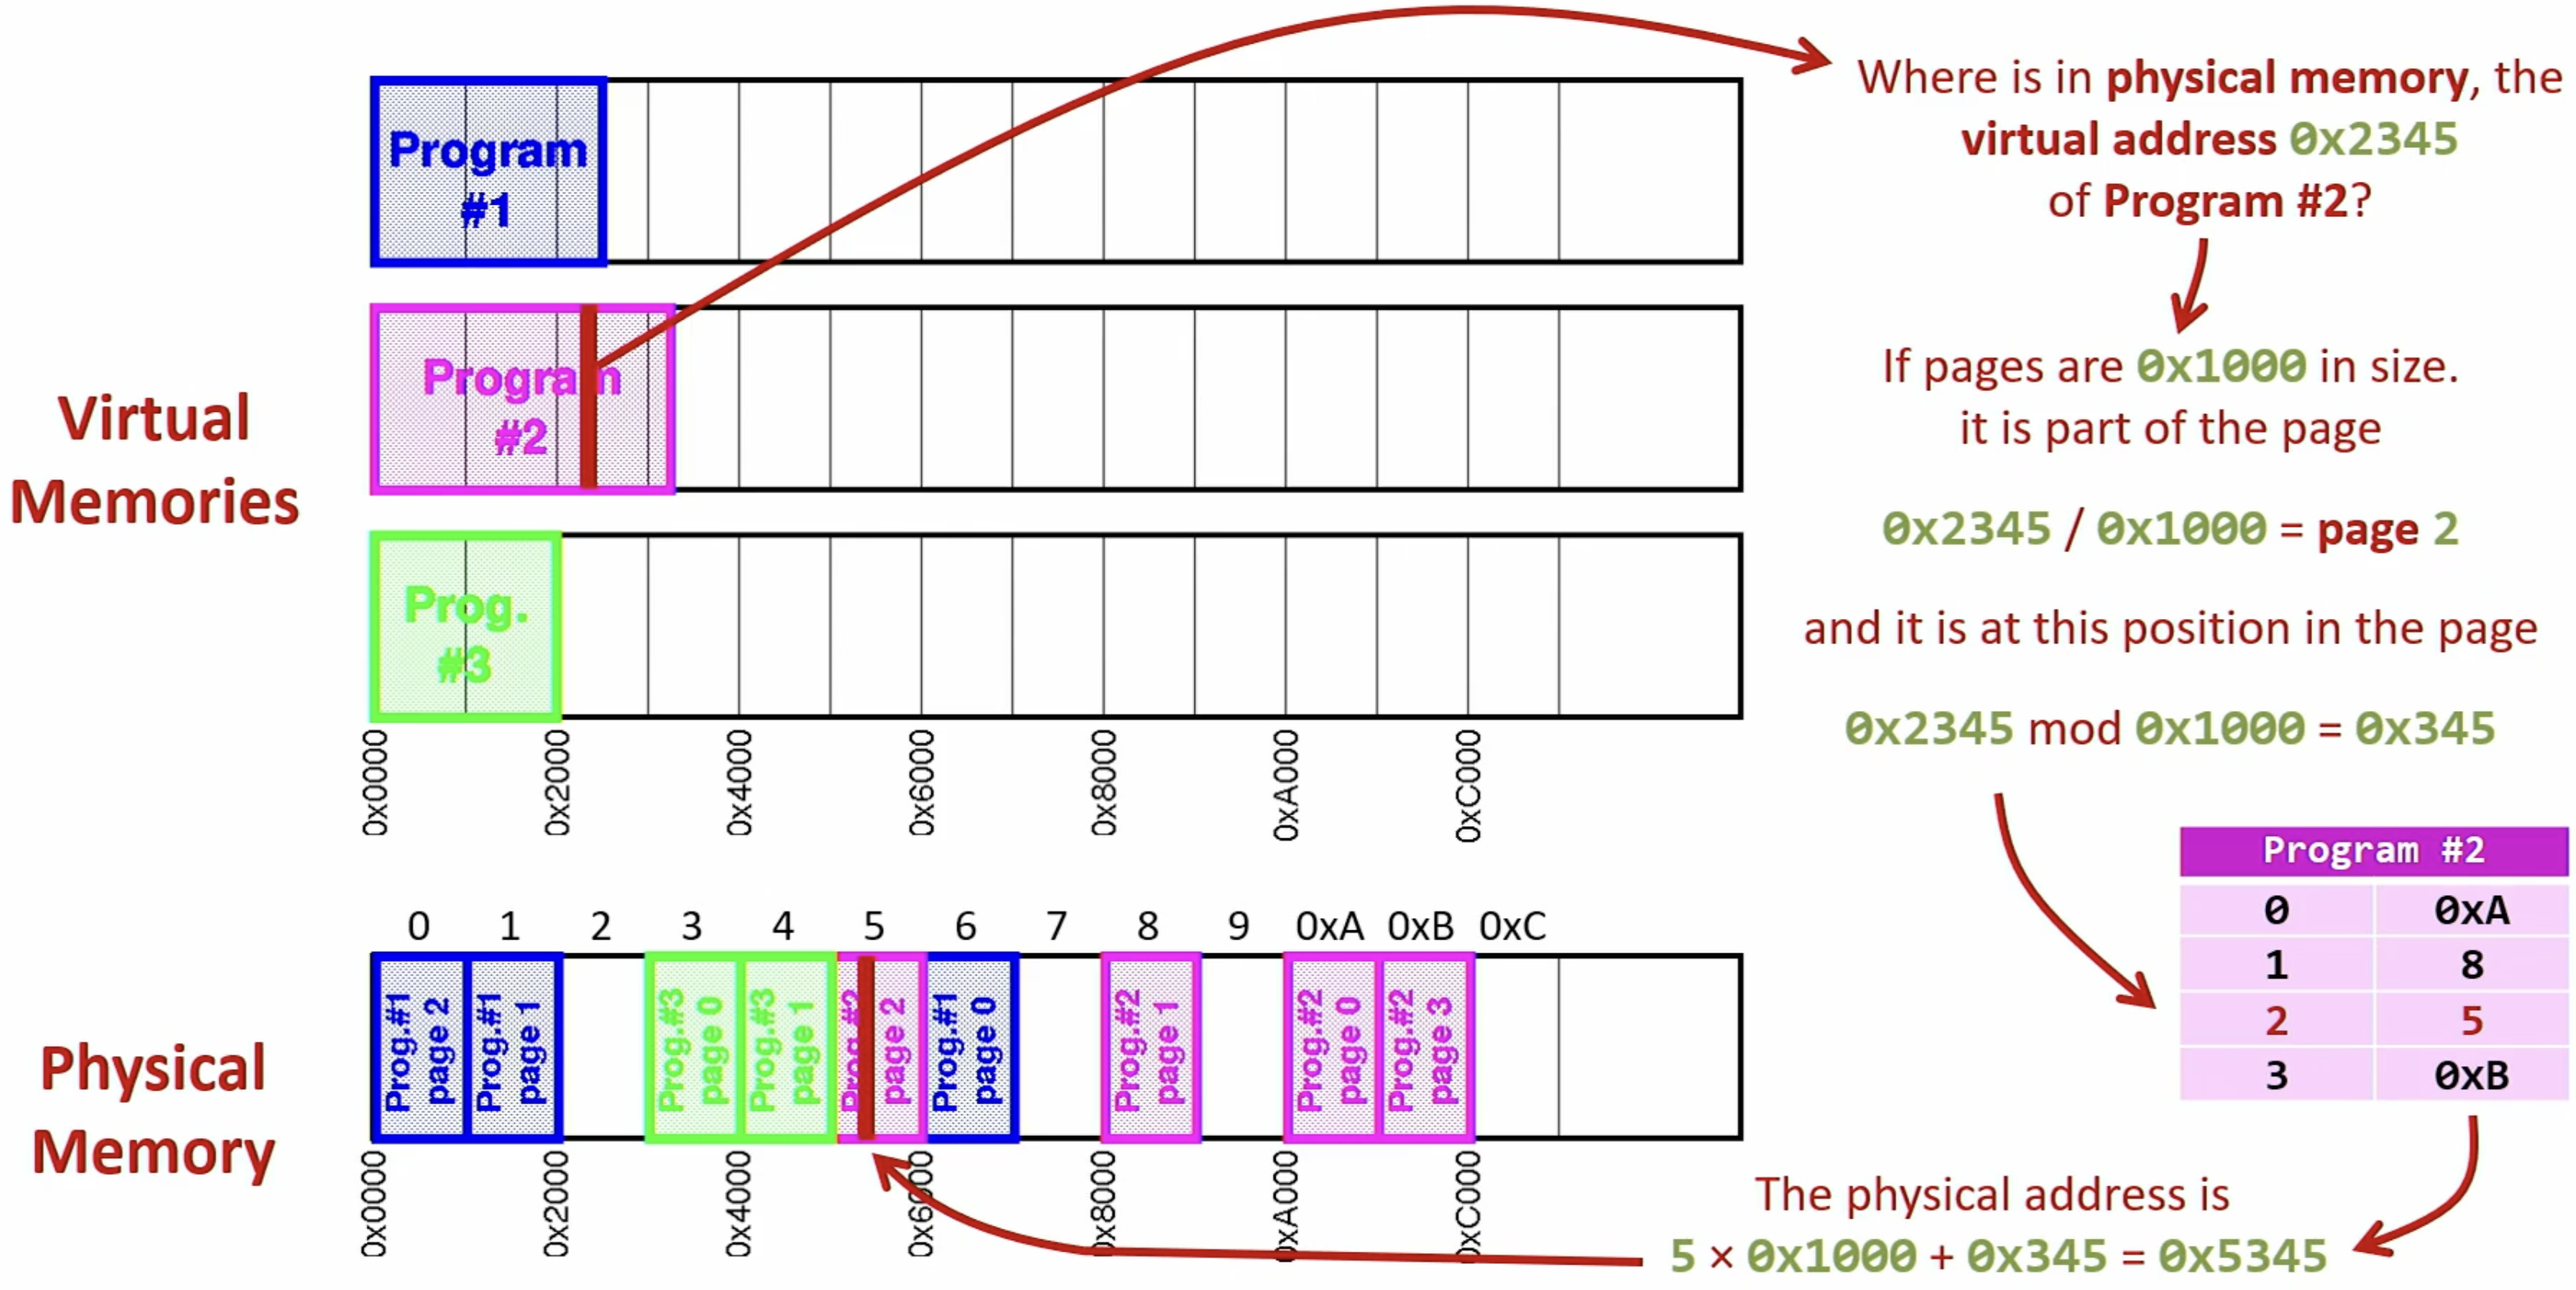
\includegraphics[width=0.65\textwidth]{chapters/chapter3c/images/translate.png}
\end{center}

For example,if the system needs to determine the physical memory location corresponding to the virtual address \texttt{0x2345} of \textbf{Program \#2}. The translation process follows these steps:

\begin{enumerate}
    \item Identify the \textbf{page number} and \textbf{offset} within the virtual address. Assuming page size is known, \texttt{0x2345} translates to a specific page and offset.
    \item Consult the \textbf{page table} for \textbf{Program \#2}, which maps virtual pages to physical pages. For instance:
    \[
    \text{\texttt{Program \#2 Page 0}} \rightarrow \text{\texttt{Physical Page 8}}, \quad
    \text{\texttt{Page 1}} \rightarrow \text{\texttt{Physical Page 9}}
    \]
    \item Use the mapping to locate the physical address. In this example, the virtual address resides in \texttt{Page 0}, which maps to \texttt{Physical Page 8}. Combining the physical page base address with the offset yields the final physical memory address.
\end{enumerate}

Sumarized, to find the physical address, we need to extract the virtual page number and the page offset from the virtual address. The virtual page number is used to look up the corresponding physical frame number in the page table. Finally, the physical address is computed using the formula:
\begin{center}
    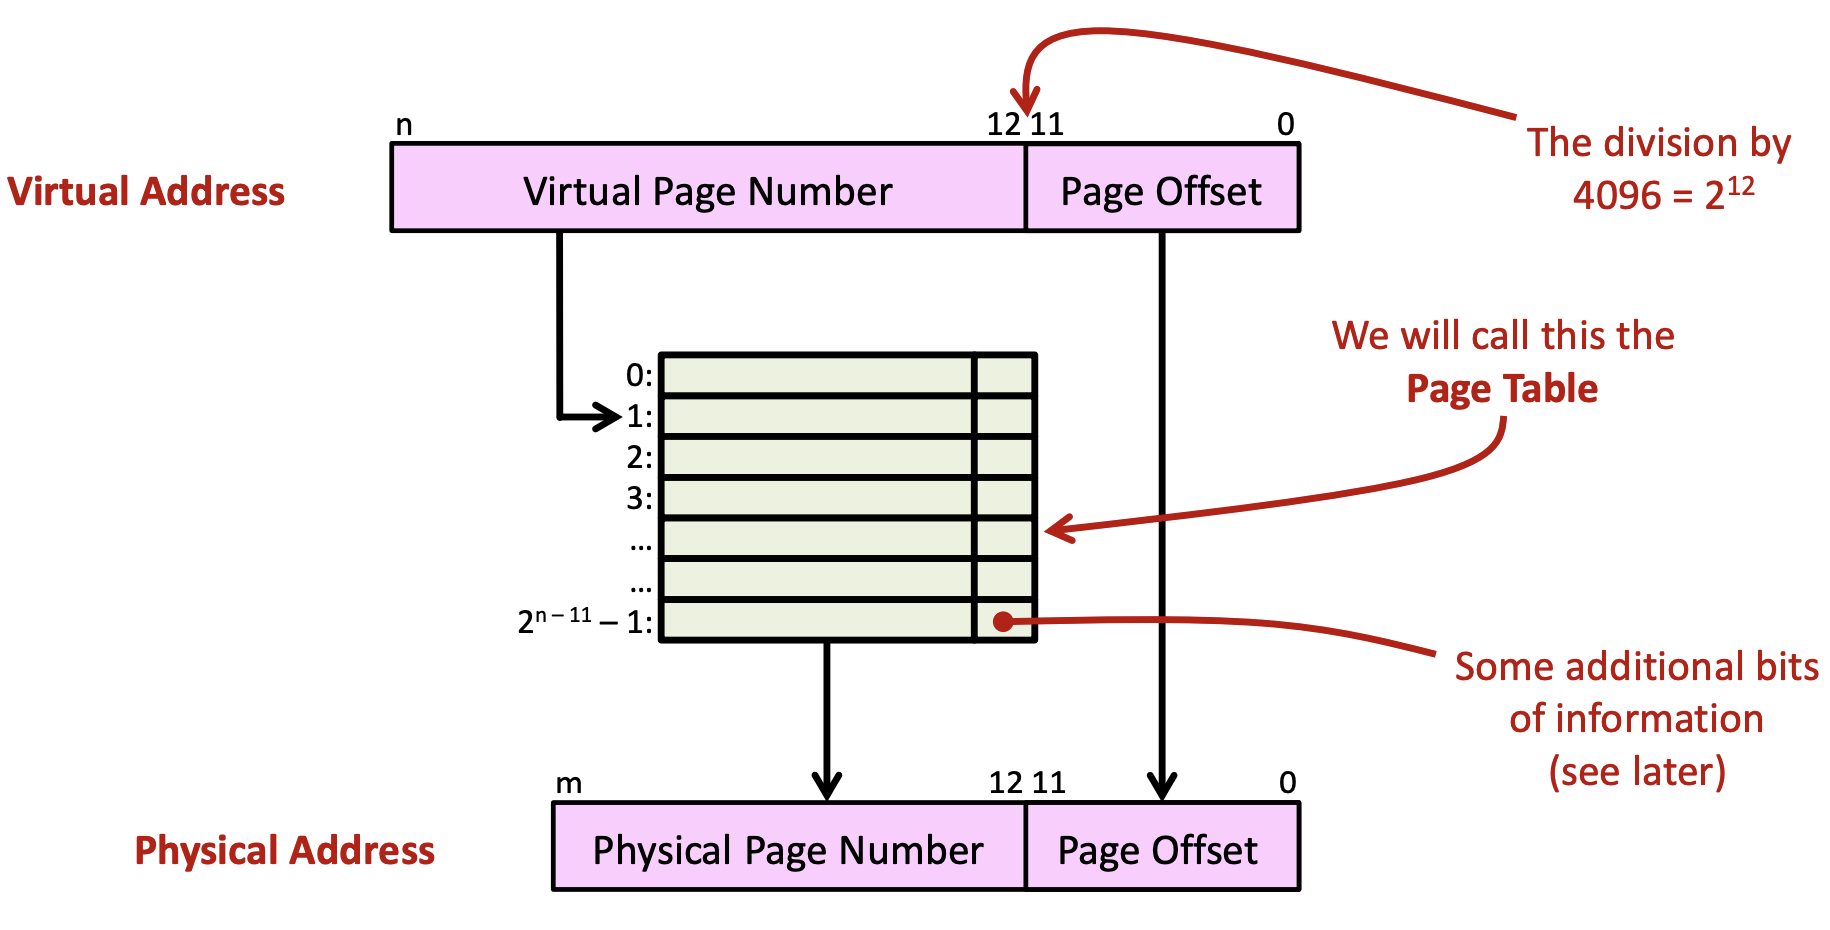
\includegraphics[width=0.65\textwidth]{chapters/chapter3c/images/translate2.png}
\end{center}
\[
\text{Physical Address} = (\text{Physical Frame Number} \times \text{Page Size}) + \text{Page Offset}
\]

where the page offset is directly derived from the virtual address, and the physical frame number is obtained from the page table. The page size is often a power of 2 (for example, \(4 \, \text{KB} = 2^{12}\)), which makes extracting the page offset straightforward as it corresponds to the lower-order bits of the virtual address.
\newpage
\subsection{Virtual Adress Translation in a Paged MMU}
In a paged MMU, the virtual address generated by the processor is translated into a physical address using the page table stored in memory.
\begin{center}
    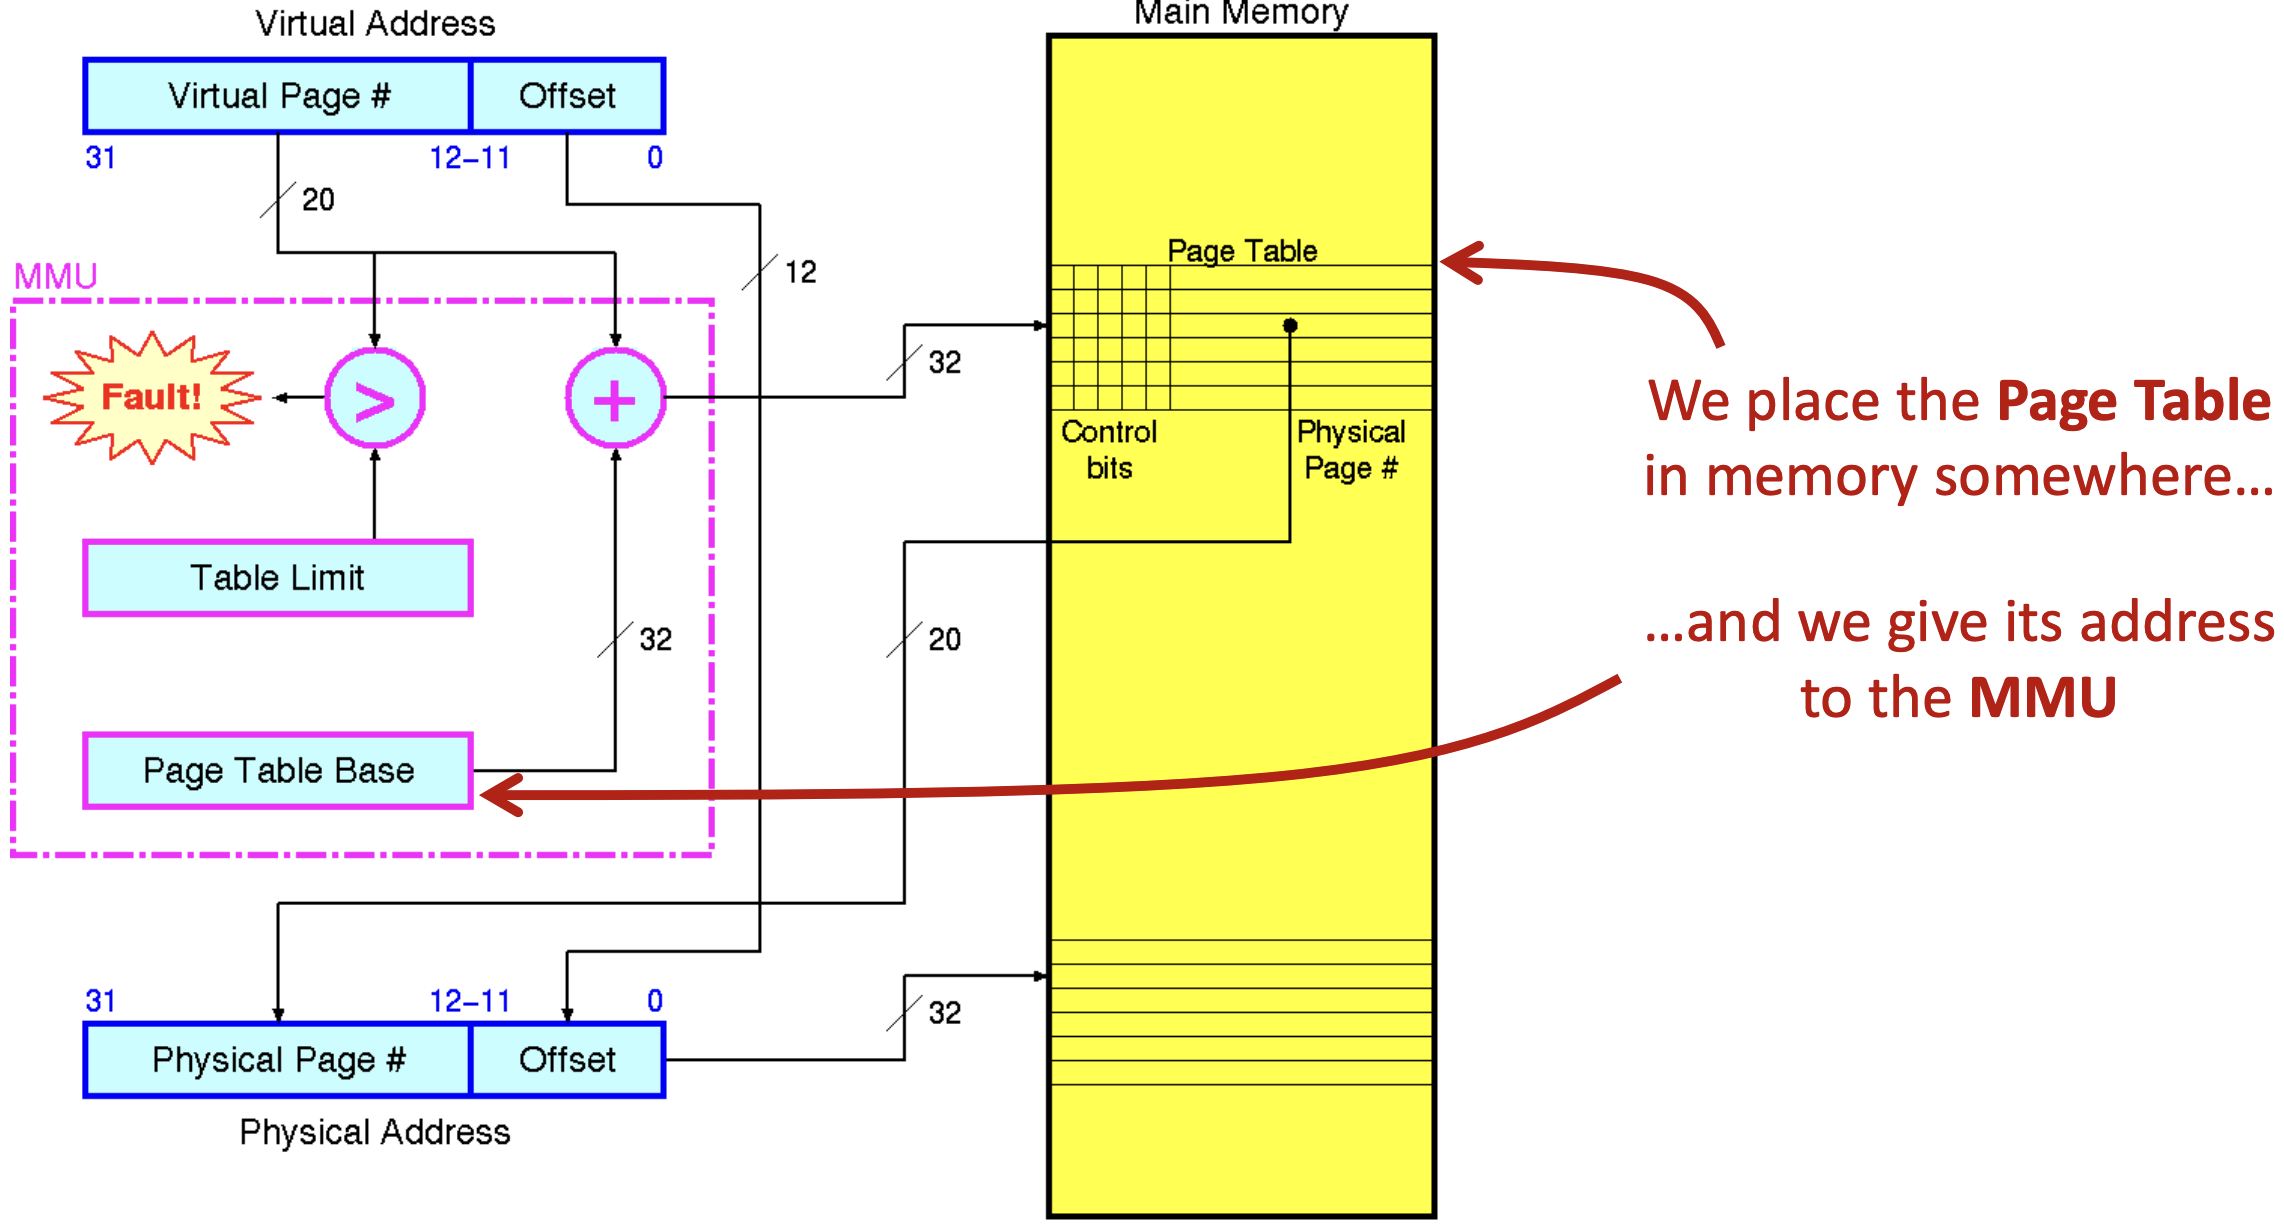
\includegraphics[width=0.65\textwidth]{chapters/chapter3c/images/pagedmmu.png}
\end{center}

\begin{itemize}
    \item[] \textbf{Page Table:}
    The page table, residing in main memory, contains:
    \begin{itemize}
        \item \textit{Control Bits:} Indicate the validity of a page and access permissions.
        \item \textit{Physical Page Numbers:} Map virtual pages to physical pages.
    \end{itemize}
\end{itemize}

\subsection{Memory Allocation is Easy Now}
Virtual memory systems simplify memory allocation by allowing noncontiguous physical memory to be mapped to contiguous virtual memory addresses. This enables efficient utilization of physical memory without requiring large, contiguous blocks.
\begin{center}
    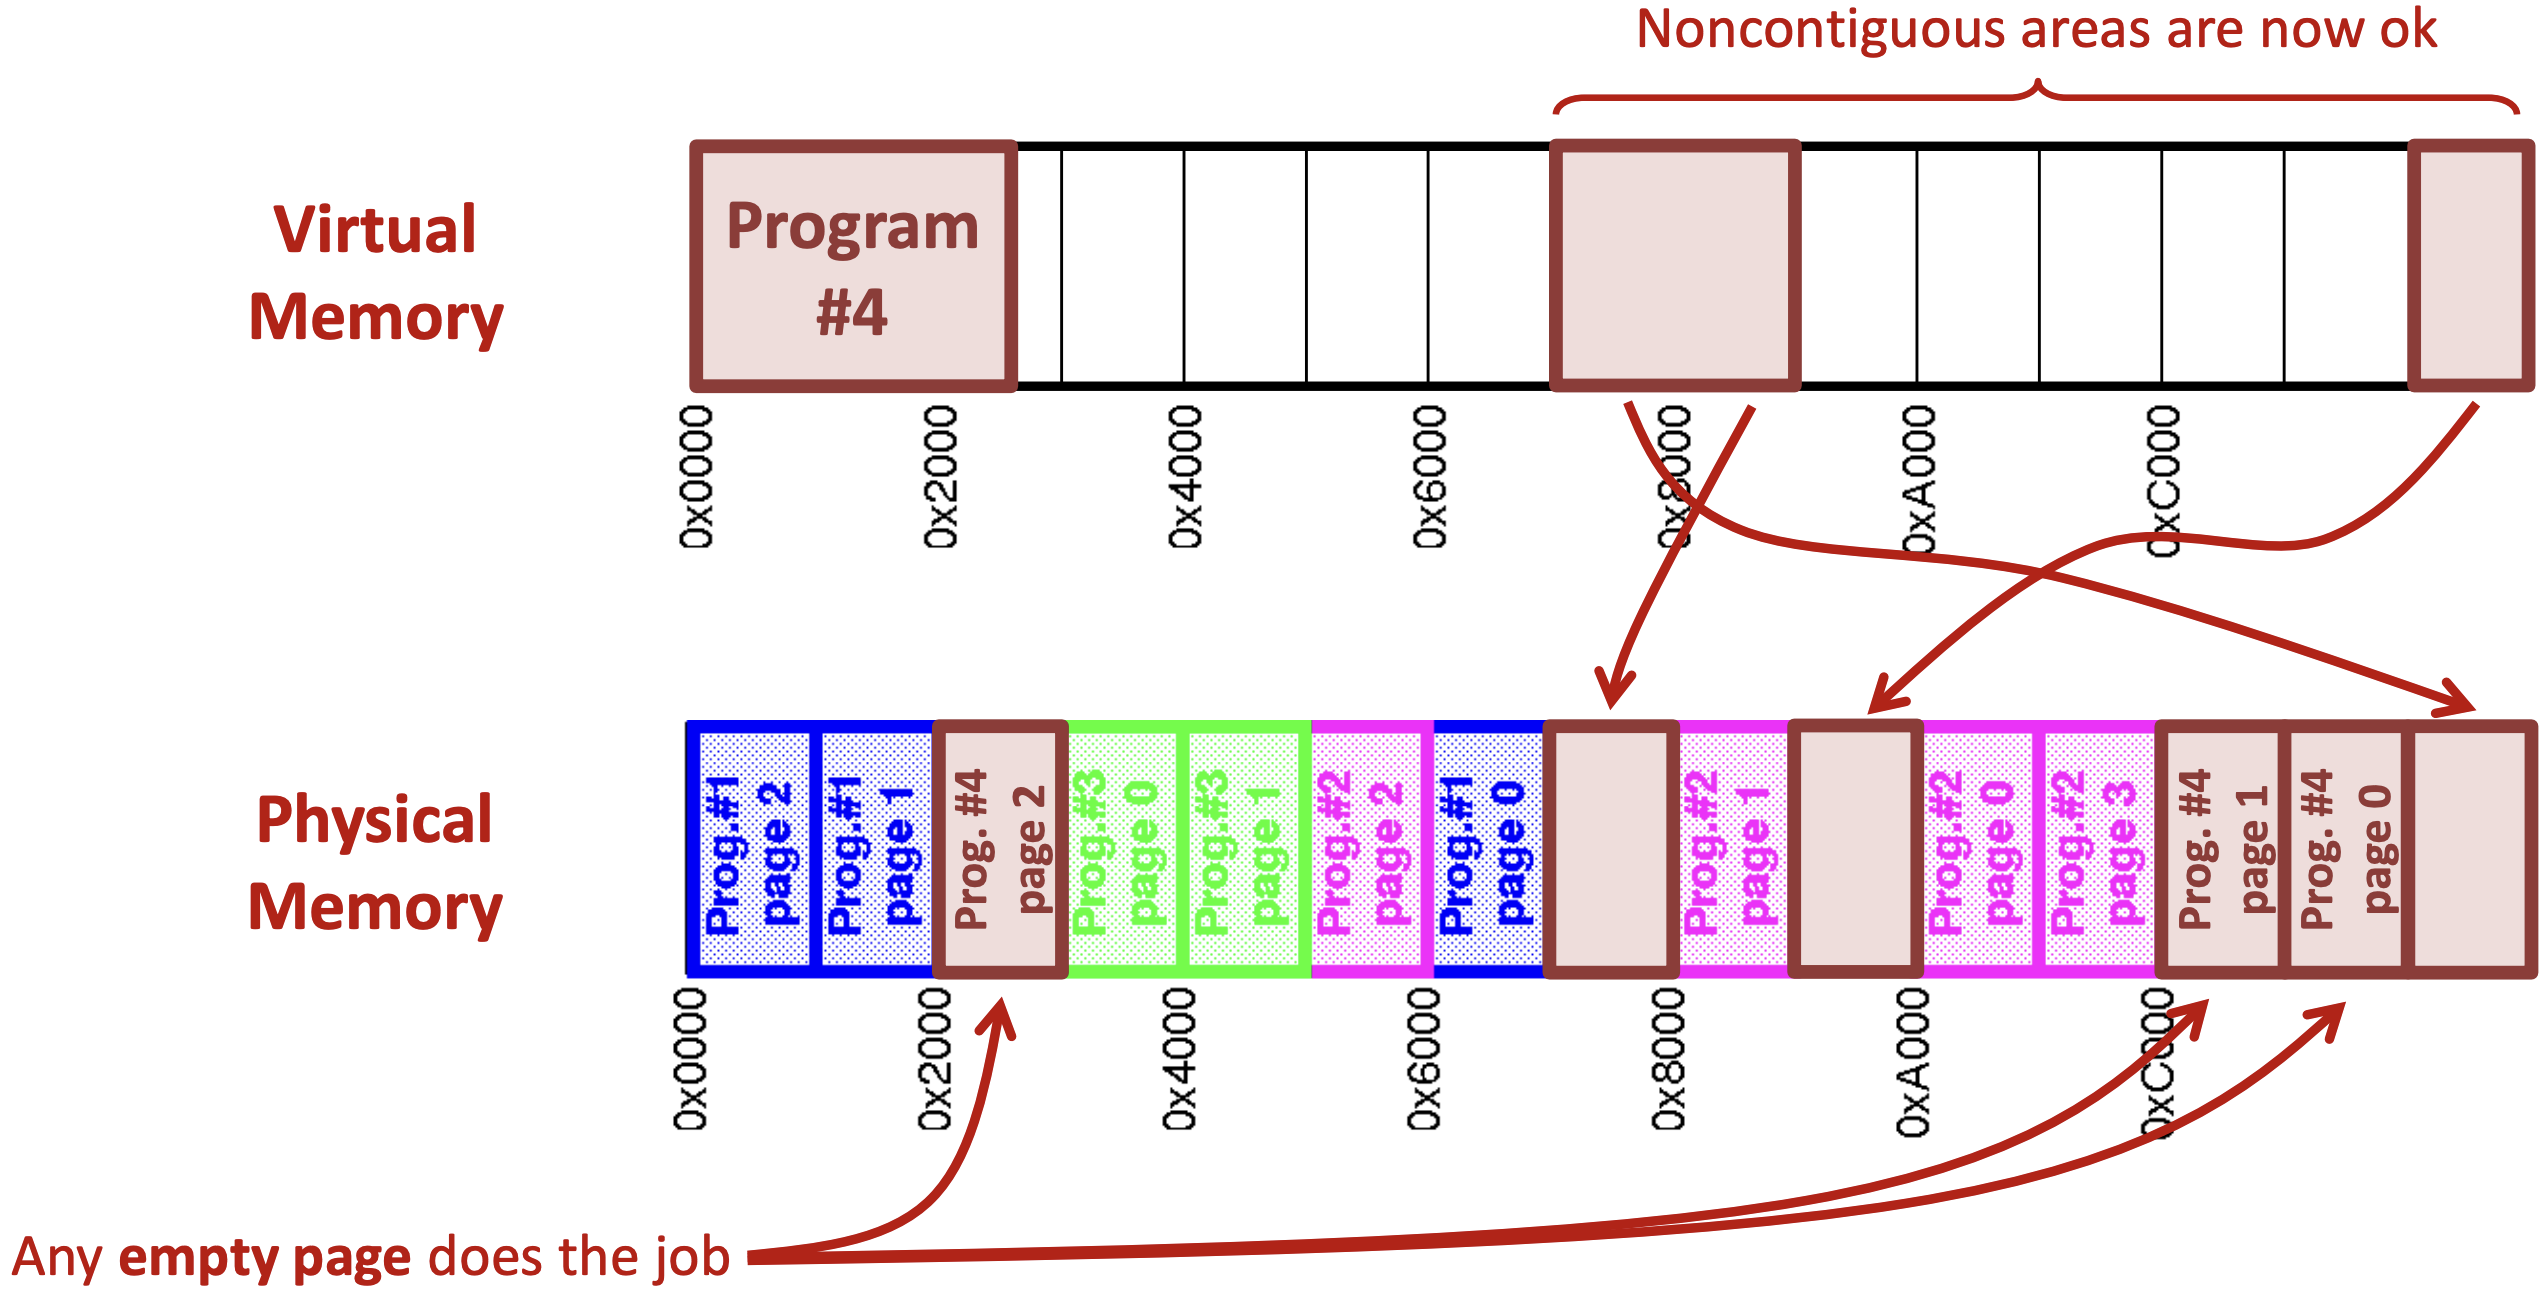
\includegraphics[width=0.65\textwidth]{chapters/chapter3c/images/relocation_bis.png}
\end{center}
\begin{itemize}
    \item[] \textbf{Virtual Memory:} Each program operates in its own virtual address space, making it unaware of the physical memory layout. Virtual addresses are mapped to physical addresses using a page table.
    \item[] \textbf{Physical Memory:} Physical memory is divided into fixed-size blocks called \textit{pages}. Any empty page in physical memory can be allocated to a program's virtual page.
    \item[] \textbf{Advantages:}
    \begin{itemize}
        \item Programs can use noncontiguous memory regions without manual intervention.
        \item Memory fragmentation is minimized since any available physical page can be used.
        \item Programs are isolated from one another, enhancing security and stability.
    \end{itemize}
    \item[] In the diagram above, Program \#4's virtual memory is mapped to noncontiguous pages in physical memory (e.g., 0x2000, 0x8000, and 0xC000). This flexibility ensures efficient allocation.
\end{itemize}

The use of virtual memory significantly enhances system performance and simplifies memory management by abstracting physical memory complexities.

\subsection{Page Tables and Their Size}
Page tables in virtual memory systems can grow significantly in size, especially in cases with large memory spaces. For instance, a memory size of 64 GiB with 4 KiB pages requires $2^{24}$ entries, amounting to approximately 64 MiB of space.

\textbf{Challenges} \\
For programs that utilize only a few megabytes, the majority of these entries remain empty, leading to inefficient memory usage.

\textbf{Solutions} \\
Several approaches exist to mitigate this inefficiency, including:
\begin{itemize}
    \item \textbf{Hashed Tables:} An alternative structure to reduce unused entries.
    \item \textbf{Paged Segmentation:} A hybrid approach to manage memory.
    \item \textbf{Multilevel Page Tables:} A hierarchical design to handle sparse page tables efficiently.
\end{itemize}

\subsection{Multilevel Page Tables}

Multilevel page tables are a hierarchical solution to reduce memory overhead caused by storing a single large page table. This structure is particularly useful in virtual memory systems with large address spaces.

\begin{center}
    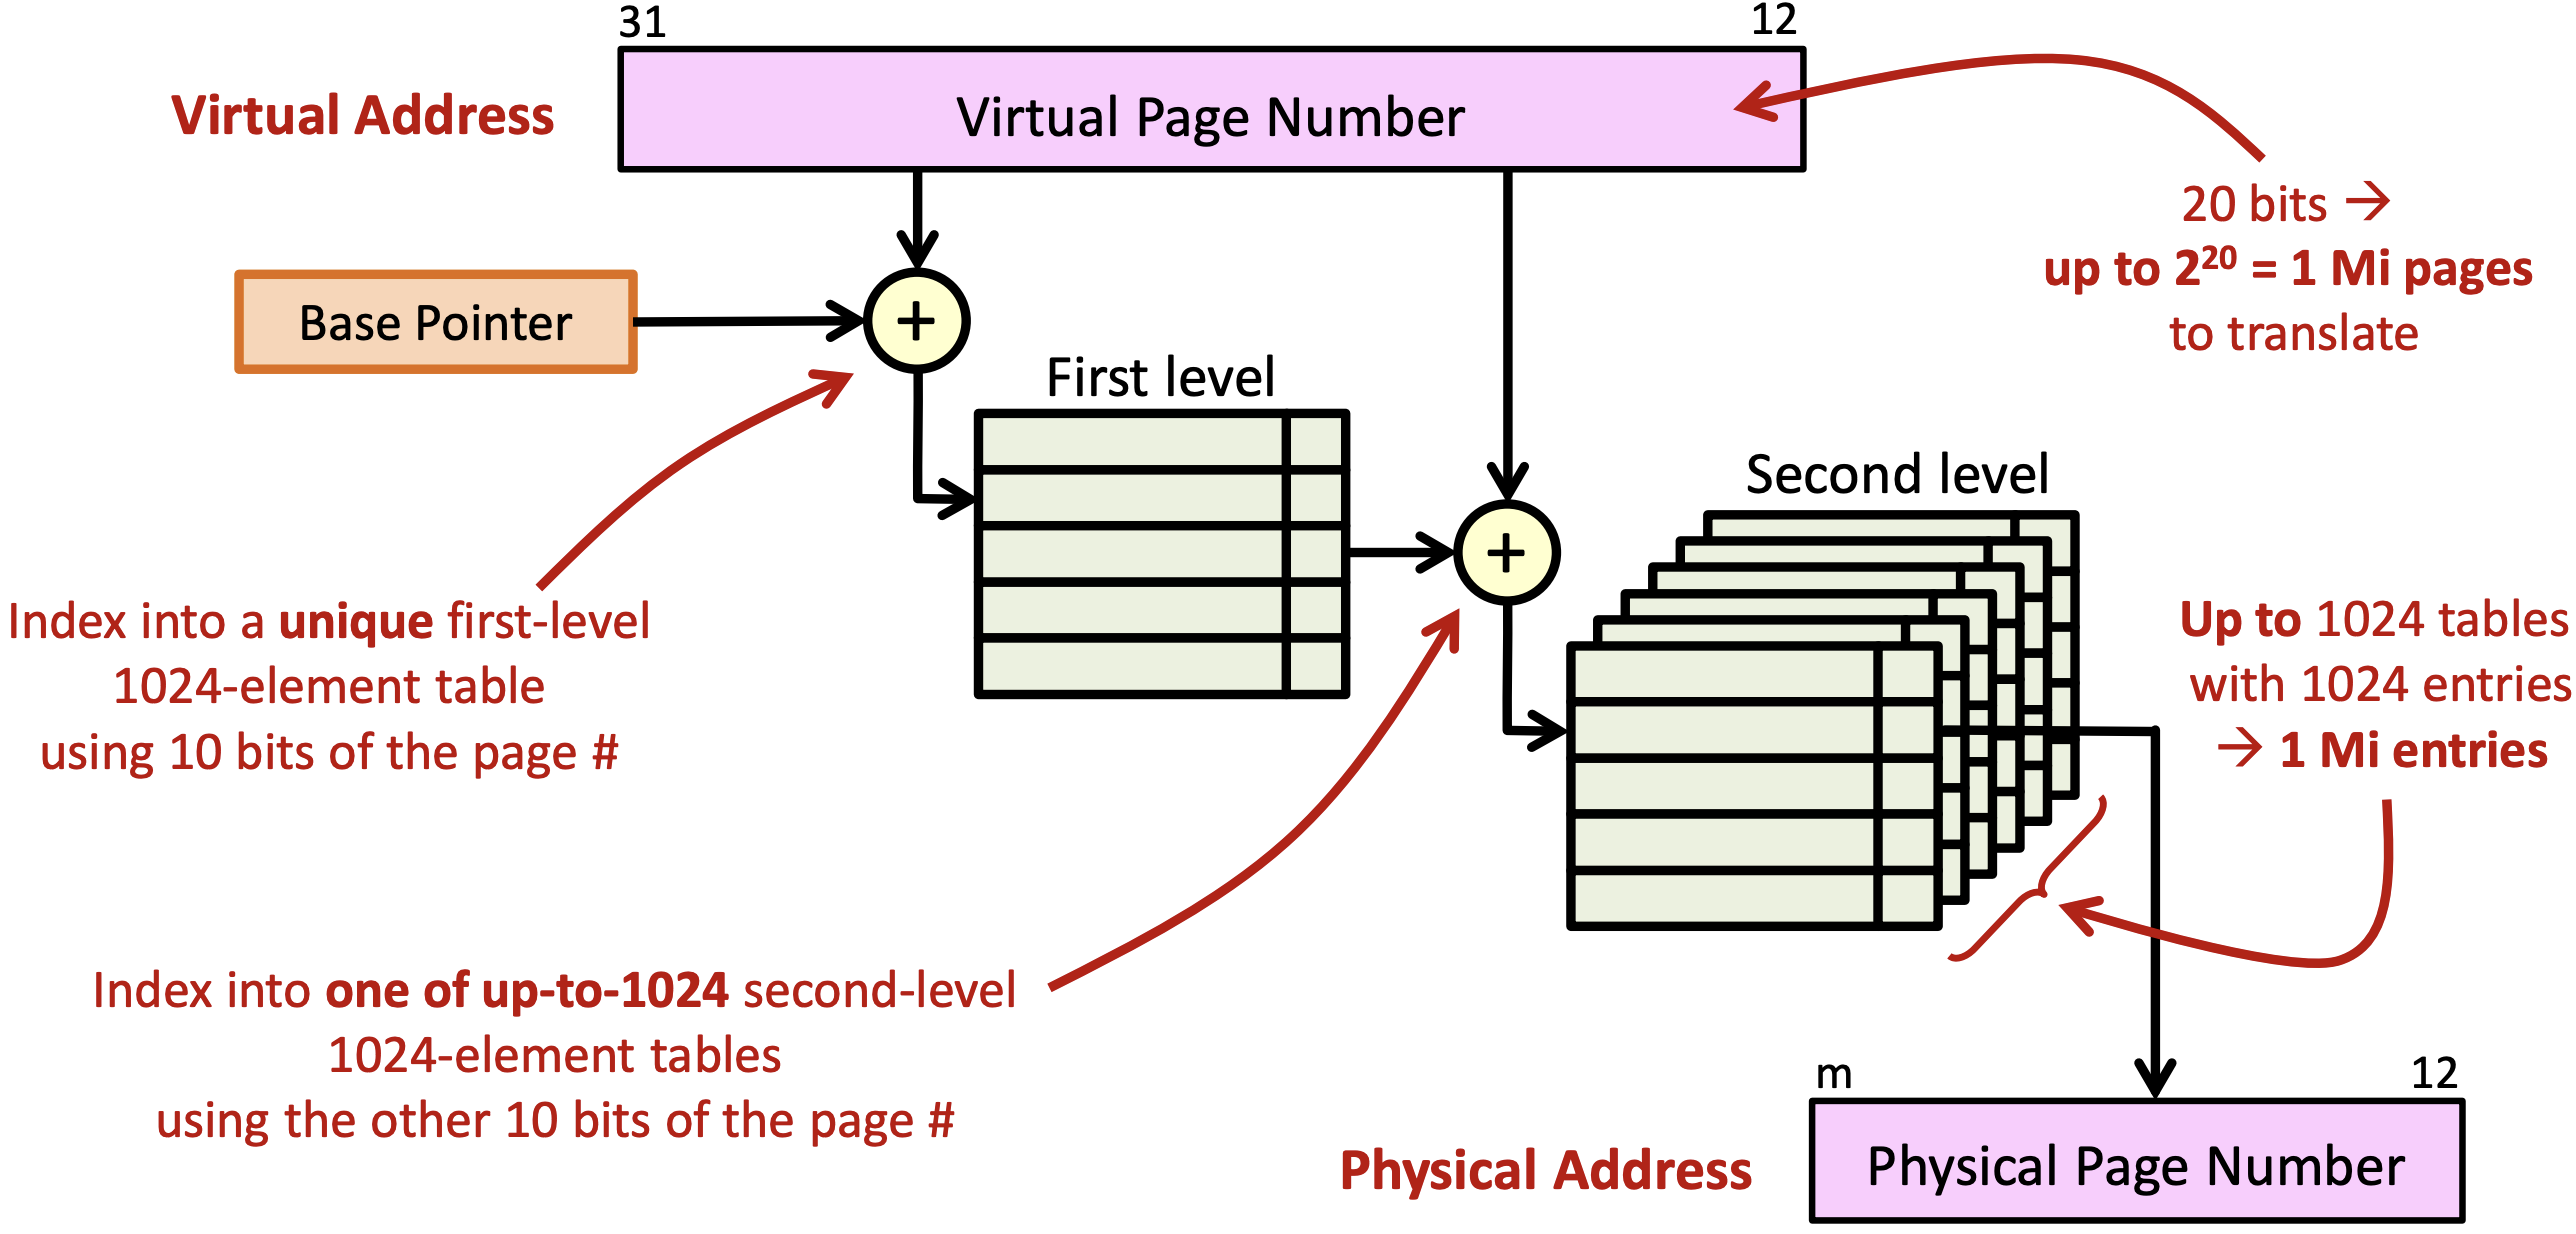
\includegraphics[width=0.65\textwidth]{chapters/chapter3c/images/multipage.png}
\end{center}
A virtual address is divided into three main parts:
\begin{itemize}
    \item \textbf{Virtual Page Number:} Determines the index within the page tables.
    \item \textbf{Page Offset:} Specifies the exact byte within the page.
\end{itemize}

The hierarchical organization involves:
\begin{enumerate}
    \item A \textbf{first-level page table}, indexed by the higher-order bits of the virtual page number. This table points to second-level page tables.
    \item \textbf{Second-level page tables}, indexed by the remaining bits of the virtual page number. These map to the physical page number.
\end{enumerate}

\textbf{Advantages:} \\
\begin{itemize}
    \item \textbf{Reduced memory usage:} Only necessary parts of the page tables are stored in memory.
    \item \textbf{Scalability:} Easily adapts to varying address space sizes.
\end{itemize}

\textbf{Key Steps in Address Translation:} \\
\begin{enumerate}
    \item Use the first-level index to locate the appropriate second-level page table.
    \item Use the second-level index to identify the physical page number.
    \item Combine the physical page number with the page offset to obtain the physical address.
\end{enumerate}

Multilevel page tables strike a balance between efficiency and memory overhead, making them a practical choice in modern operating systems.

 % Including chapter0.tex from chapters folder
\chapter{Comparch II - Part 4a. Instruction Level Parallelism Performance}
\textit{So far, we've only been building our processor, now it's about performance\dots}
\section{What is Performance ?}
\textit{Now what do we mean by performance ?, we need a metric to measure performance.}
\begin{itemize}
    \item[] Does processory frequency matter ? \textit{Is it better an Intel Core i7-7700K at 4.2 GHz or an AMD Ryzen 5 5600X at 3.7 GHz?}
    \item[] Memory Speed ? Cache efficiency ?
    \begin{itemize}
        \item[] Is it better to have 8 MiB of 4-way set-associative cache or 16 MiB of direct
        mapped cache?
        \item[] Is it better to have three levels of overall smaller caches or two levels of overall
        bigger caches?
    \end{itemize}
\end{itemize}
\subsection{Elapsed Time, CPU Time, \dots}
\textit{In reality, none of this matters in it self.}
What matters is the time it takes to perform a job a user needs.
\begin{center}
    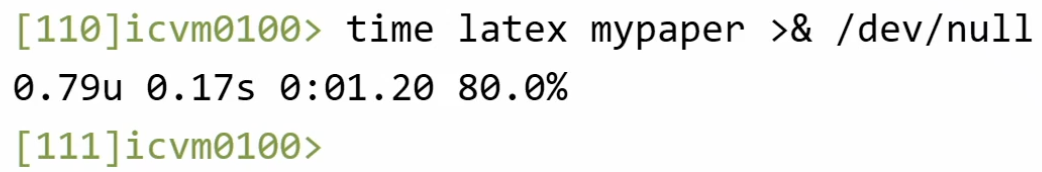
\includegraphics[width=0.45\textwidth]{chapters/chapter4a/images/elapsed.png}
\end{center}

\begin{itemize}
    \item \textbf{Elapsed Time:} The total time taken for the job to complete, measured from start to finish. (e.g., 1.20 seconds)
    \item \textbf{System CPU Time:} The CPU time used by the operating system to execute instructions on behalf of the program. (e.g., 0.17 seconds)
    \item \textbf{User CPU Time:} The CPU time used to execute instructions for the program itself. (e.g., 0.79 seconds)
    \item 80.0\% of the Elapsed Time ($0.96\,s / 1.20\,s$) was spent on the job (the rest might be spent on system I/O, other jobs, and other users.)
    \item \textbf{Note:} \textit{User CPU Time} + \textit{System CPU Time} $\neq$ \textit{Elapsed Time}: The processor spent 0.96 seconds executing for the program, but the overall job took 1.20 seconds to complete.
\end{itemize}

\subsection{Relative Performance}
\textbf{Speedup}

The speedup metric quantifies how much faster system $X$ is compared to system $Y$. It is defined as:
\[
\text{Speedup} = \frac{\text{Performance}_X}{\text{Performance}_Y} = \frac{\text{Execution Time}_Y}{\text{Execution Time}_X}
\]

\textbf{Common Performance Indices}
Common benchmarks used to measure the speedups of systems relative to a standard system include: \newline
\textbf{SPEC CPU} (a classic CPU performance benchmark), \textbf{Geekbench} (a comprehensive cross-platform benchmark), \textbf{Cinebench} (a benchmark focusing on rendering performance), \textbf{LinPack HPL} (a high-performance computing benchmark), and \textbf{EEMBC (``Embassy'') CoreMark} (dedicated to benchmarking embedded processors).

\subsection{Relating Performance to Hardware Implementation}
In hardware design, time is measured by the \textit{clock period} or \textit{cycle}.

\subsubsection{Cycles per Instruction (CPI) and Instructions per Cycle (IPC)}
\begin{itemize}
    \item CPI: Average cycles needed per instruction
    \[
    \text{CPI} = \frac{\text{Total Cycles}}{\text{Total Instructions}} = \frac{\text{Execution Time}/\text{Clock Period}}{\text{Total Instructions}}
    \]
    \item IPC: Average instructions executed per cycle
    \[
    \text{IPC} = \frac{1}{\text{CPI}}
    \]
    \item Note: IPC $\leq$ 1 unless the processor can execute multiple instructions in parallel
\end{itemize}

\subsection{Improving Performance}
Performance is defined as the reciprocal of execution time:

\[
\text{Performance} = \frac{1}{\text{Execution Time}}
\]

By breaking down execution time, performance can be expressed as:

\[
\text{Performance} = \frac{f_{\text{clock}}}{\text{Instruction Count} \cdot \text{CPI}} = \frac{f_{\text{clock}}\cdot IPC}{\text{Instruction Count}}
\]

Where:
\begin{itemize}
    \item[] $f_{\text{clock}}$ is the clock frequency.
    \item[] $\text{CPI}$ is the cycles per instruction.
    \item[] $\text{Instruction Count}$ is the total number of instructions executed.
\end{itemize}

To improve performance, several strategies can be employed:

\begin{enumerate}
    \item \textbf{Increase Clock Frequency ($f_{\text{clock}}$):} Implement the processor using faster technology to achieve higher clock rates.
    \item \textbf{Reduce CPI:} Simplify instructions (RISC architecture) to lower the cycles per instruction. However, this may require more instructions to perform the same task.
    \item \textbf{Decrease Instruction Count:} Use fewer, more complex instructions (CISC architecture). This could increase the number of cycles per instruction or reduce the clock frequency.
    \item \textbf{Execute Instructions in Parallel:} Increase instructions per cycle (IPC) through techniques like pipelining or parallel execution.
\end{enumerate}
These trade-offs highlight the balance required when optimizing computer architecture for performance.

\subsection{Factors Influencing Performance}
Several factors can significantly impact system performance. Here are a few examples:

\begin{itemize}
    \item \textbf{Instruction Count and the Compiler:}
    \begin{itemize}
        \item The instruction count depends heavily on the compiler.
        \item A well-designed instruction set that the compiler can use effectively (i.e., best instructions for the job) is more important than having a highly reduced or overly complex instruction set. Otherwise, the instruction count may become unnecessarily large.
    \end{itemize}

    \item \textbf{Cycles Per Instruction (CPI) and Cache Performance:}
    \begin{itemize}
        \item CPI is influenced by the efficiency of the cache.
        \item As the overall code size increases, cache performance may degrade due to a higher number of cache misses.
    \end{itemize}

    \item \textbf{Clock Cycle Speed and Memory Access:}
    \begin{itemize}
        \item Faster clock cycles increase the demand for fetching instructions from memory.
        \item As a result, the performance of the cache becomes more critical in maintaining overall efficiency.
    \end{itemize}
\end{itemize}

\subsection{What to Improve to Increase Performance}

\textbf{Amdahl's Law (Law of Diminishing Returns)}:
The performance enhancement possible with a given improvement is limited by the amount the improved feature is used. \\

\textbf{Typical Software Situation:} \\
If a program spends 20\% of its time in subroutine $X$, the maximum reduction in execution time achievable by optimizing $X$ is 20\%. This corresponds to a speedup of:
\[
\text{Speedup} = \frac{1}{1 - 0.2} = 1.25
\]

\textbf{In a Processor:} \\
If an instruction $Y$ is used only 0.1\% of the time, is it worth optimizing it? It is more practical to focus on optimizing instructions or operations used more frequently, such as those taking 20\% of the time.

What often happens is that we start optimizing the most used instructions, but then we forget that once optimized, the less used instructions become the bottleneck. So, we need to start looking at the less used instructions and optimize them, and so on.
\begin{center}
\textbf{\textcolor{red}{Look for where most of the time goes!}}
\end{center}

\subsection{Benchmarks}

\textbf{Performance Indices:} \\
Benchmarks such as SPEC CPU, Geekbench, Cinebench, LinPack HPL, and EEMBC ("Embassy") CoreMark require a \textbf{precise definition of the user job(s)} to be executed. \\

\textbf{Benchmark Suites:} \\
Serious \textbf{benchmark suites} consist of collections of large and representative user programs, spanning various areas of typical use. These suites are often agreed upon by manufacturers to ensure standardization. \\

\textbf{Key Features:} \\
Benchmark suites do not only define the programs (e.g., written in C, C++, FORTRAN, or Java), but also specify: \\
\begin{itemize}
    \item How the programs should be compiled.
    \item What data should be used during execution.
    \item The conditions under which the programs should be run.
\end{itemize}

\subsubsection{SPEC CPU2006 Integer Benchmarks}
The SPEC CPU2006 benchmark suite evaluates the performance of computer processors by running a set of standardized workloads. Below is a comparison of integer benchmarks between SPEC CPU2000 and SPEC CPU2006. The benchmarks are categorized by their description, language, and reference time (RT).


\begin{center}
    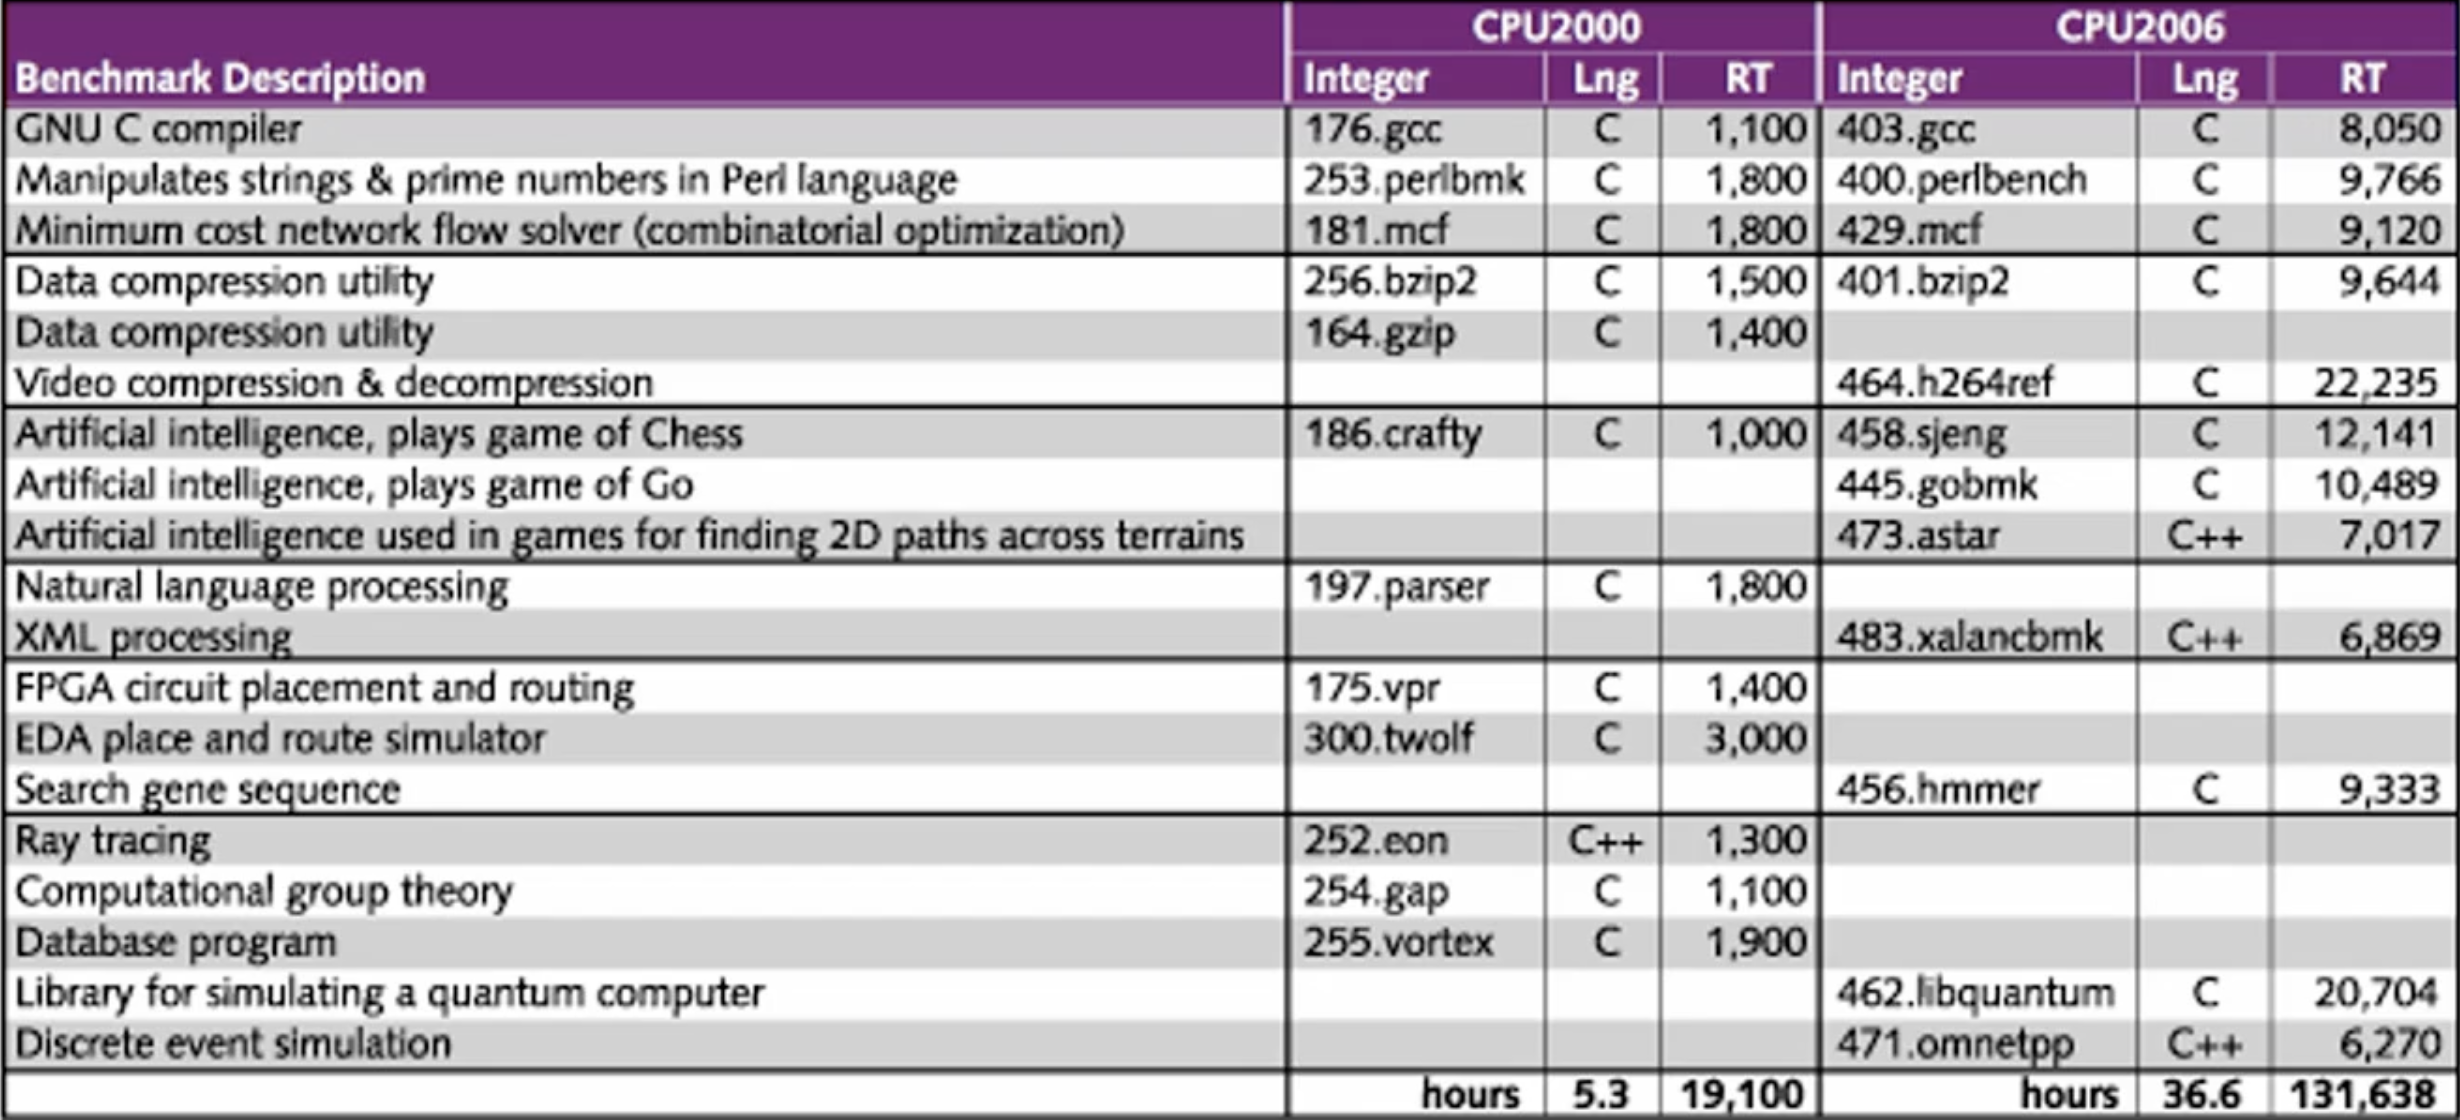
\includegraphics[width=0.65\textwidth]{chapters/chapter4a/images/spec.png}
\end{center}

\textbf{Key Notes:}
\begin{itemize}
    \item \textbf{Reference Time (RT):} Measured on a Sun Ultra 5 with a 300MHz UltraSPARC III and 256KB L2 cache, corresponding to 100 SPEC2000.
    \item \textbf{Benchmark Complexity:} The runtime for integer benchmarks was 36.6 hours on a relatively old machine.
    \item SPEC CPU2006 introduced more complex workloads and higher reference times, demonstrating a significant evolution in benchmarking standards.
\end{itemize}
 % Including chapter0.tex from chapters folder
\chapter{Part 4b. Instruction Level Parallelism Basic Pipelining}
\section{Circuit Timing and Performance}

Most of the time, we have discussed circuits at a higher level of timing abstraction, focusing on what happens during each cycle:
\begin{itemize}
    \item[-] \textbf{Finite State Machines:} $\texttt{state} \gets \texttt{next\_state}$
    \item[-] \textbf{Functional Units and Memory Elements:} Perform one operation over a small number of cycles, e.g., a combinational ALU performs an addition per cycle.
\end{itemize}

To design faster circuits, it is essential to delve deeper into the concepts of \textbf{signal propagation} and timing limitations.
\subsection{Signal Propagation}

In sequential circuits, the edges of the \texttt{clock} signal are pivotal for proper operation. They govern:

\begin{enumerate}
    \item \textbf{Data Capture}: Determining when \textbf{new data} is latched into the combinational logic.
    \item \textbf{Data Stability}: Ensuring that \textbf{processed data} (i.e., the previous input) has fully propagated through the combinational logic and is ready to be stored at the output.
\end{enumerate}

\begin{minipage}[htp]{0.45\textwidth}
    \begin{center}
        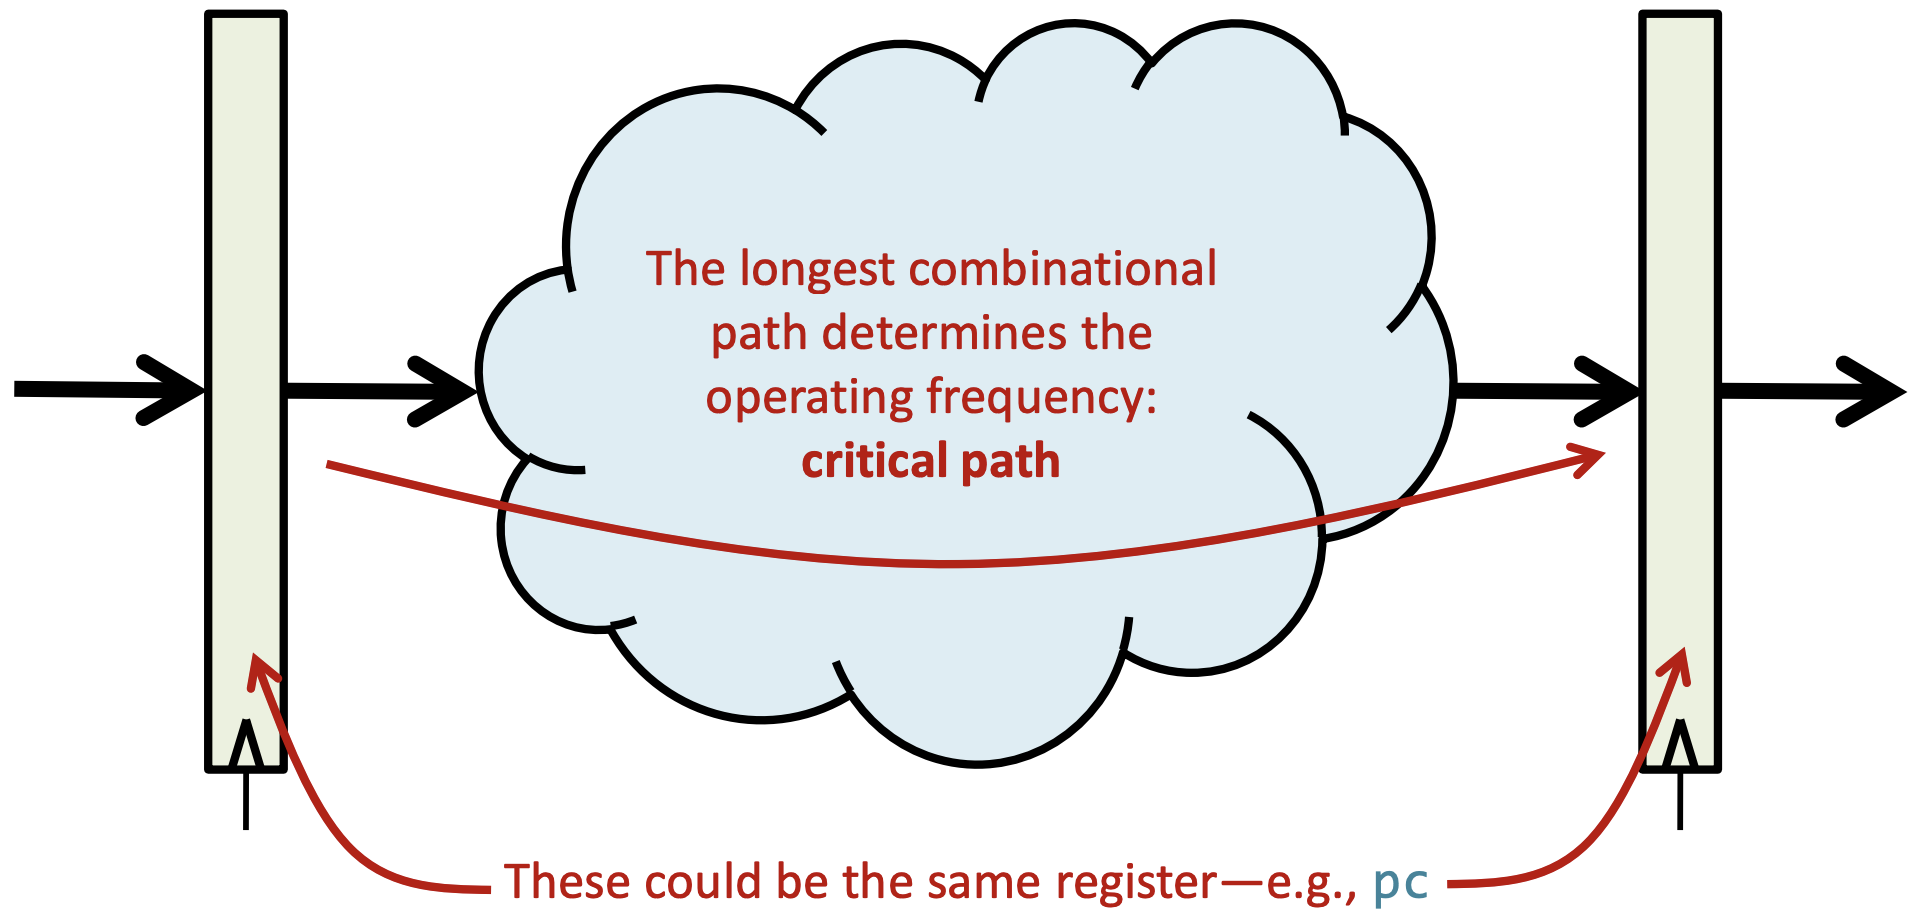
\includegraphics[width=0.45\textwidth]{chapters/chapter4b/images/prop_time.png}
    \end{center}
\end{minipage}
\hfill
\vline
\hfill
\begin{minipage}[htp]{0.45\textwidth}
    \begin{center}
        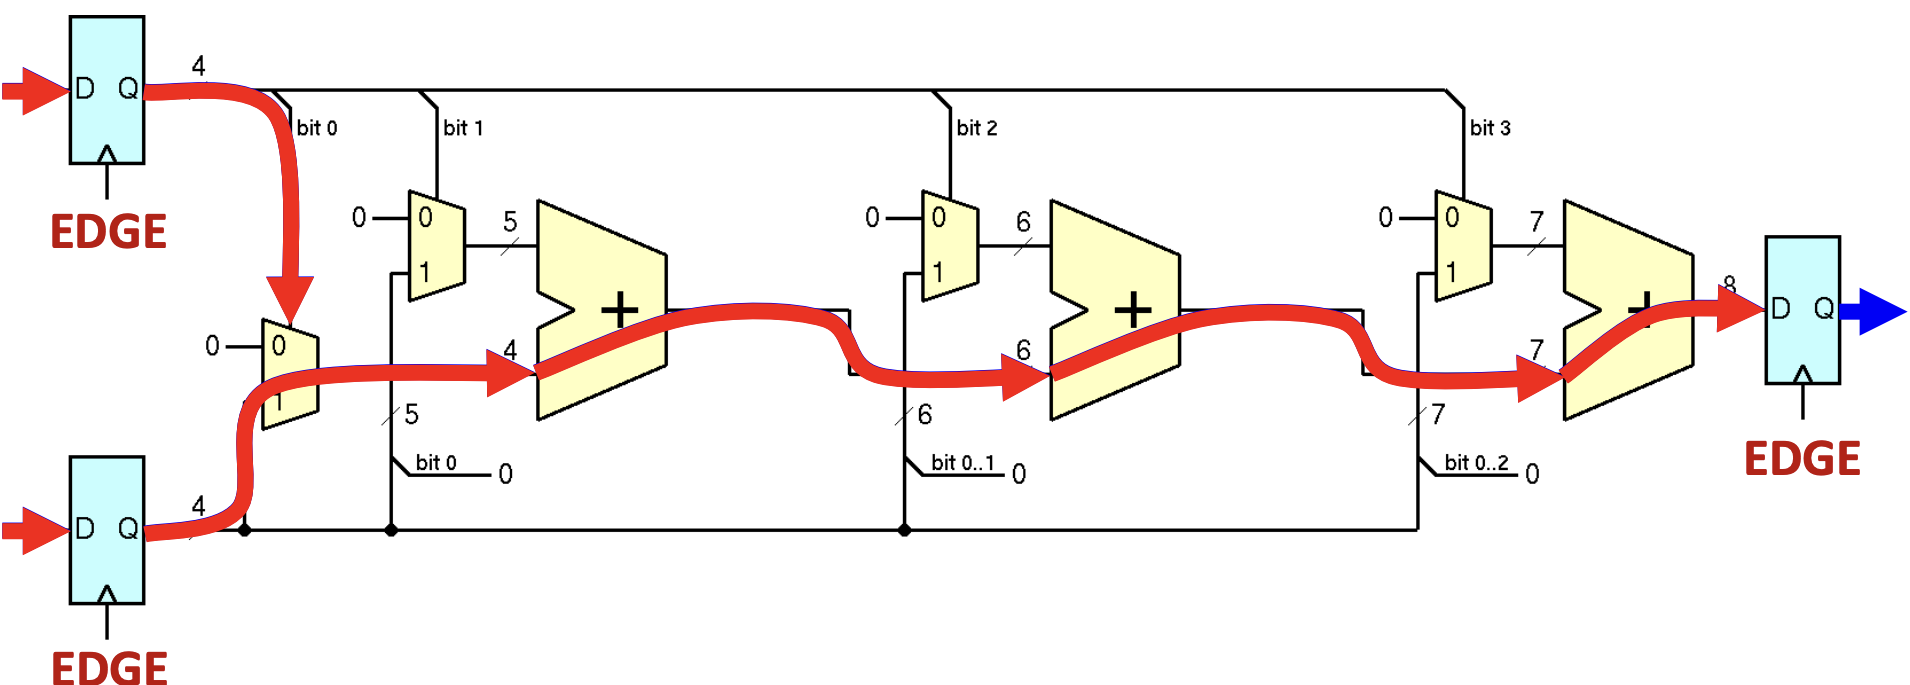
\includegraphics[width=0.65\textwidth]{chapters/chapter4b/images/prop_diag.png}
    \end{center}
\end{minipage}
To guarantee reliable operation, the \texttt{clock} period must be at least as long as the circuit's \textbf{critical path delay}—the longest delay through the combinational logic. This ensures that all signal transitions complete before the next clock edge arrives.

\[
\texttt{Clock Period} \geq \texttt{Critical Path Delay}
\]
\[
T_{\texttt{clock}} \geq T_{\texttt{critical\_path}}
\]


\noindent \textbf{Example:} In the circuit shown, the critical path is highlighted, indicating the longest combinational delay that dictates the minimum \texttt{clock} period.

\newpage

\subsubsection{Adding Intermediate Registers}
\textbf{Intermediate Registers} can be added to break up the critical path into smaller segments, reducing the overall delay. This technique is known as \textbf{pipelining}.
\begin{center}
    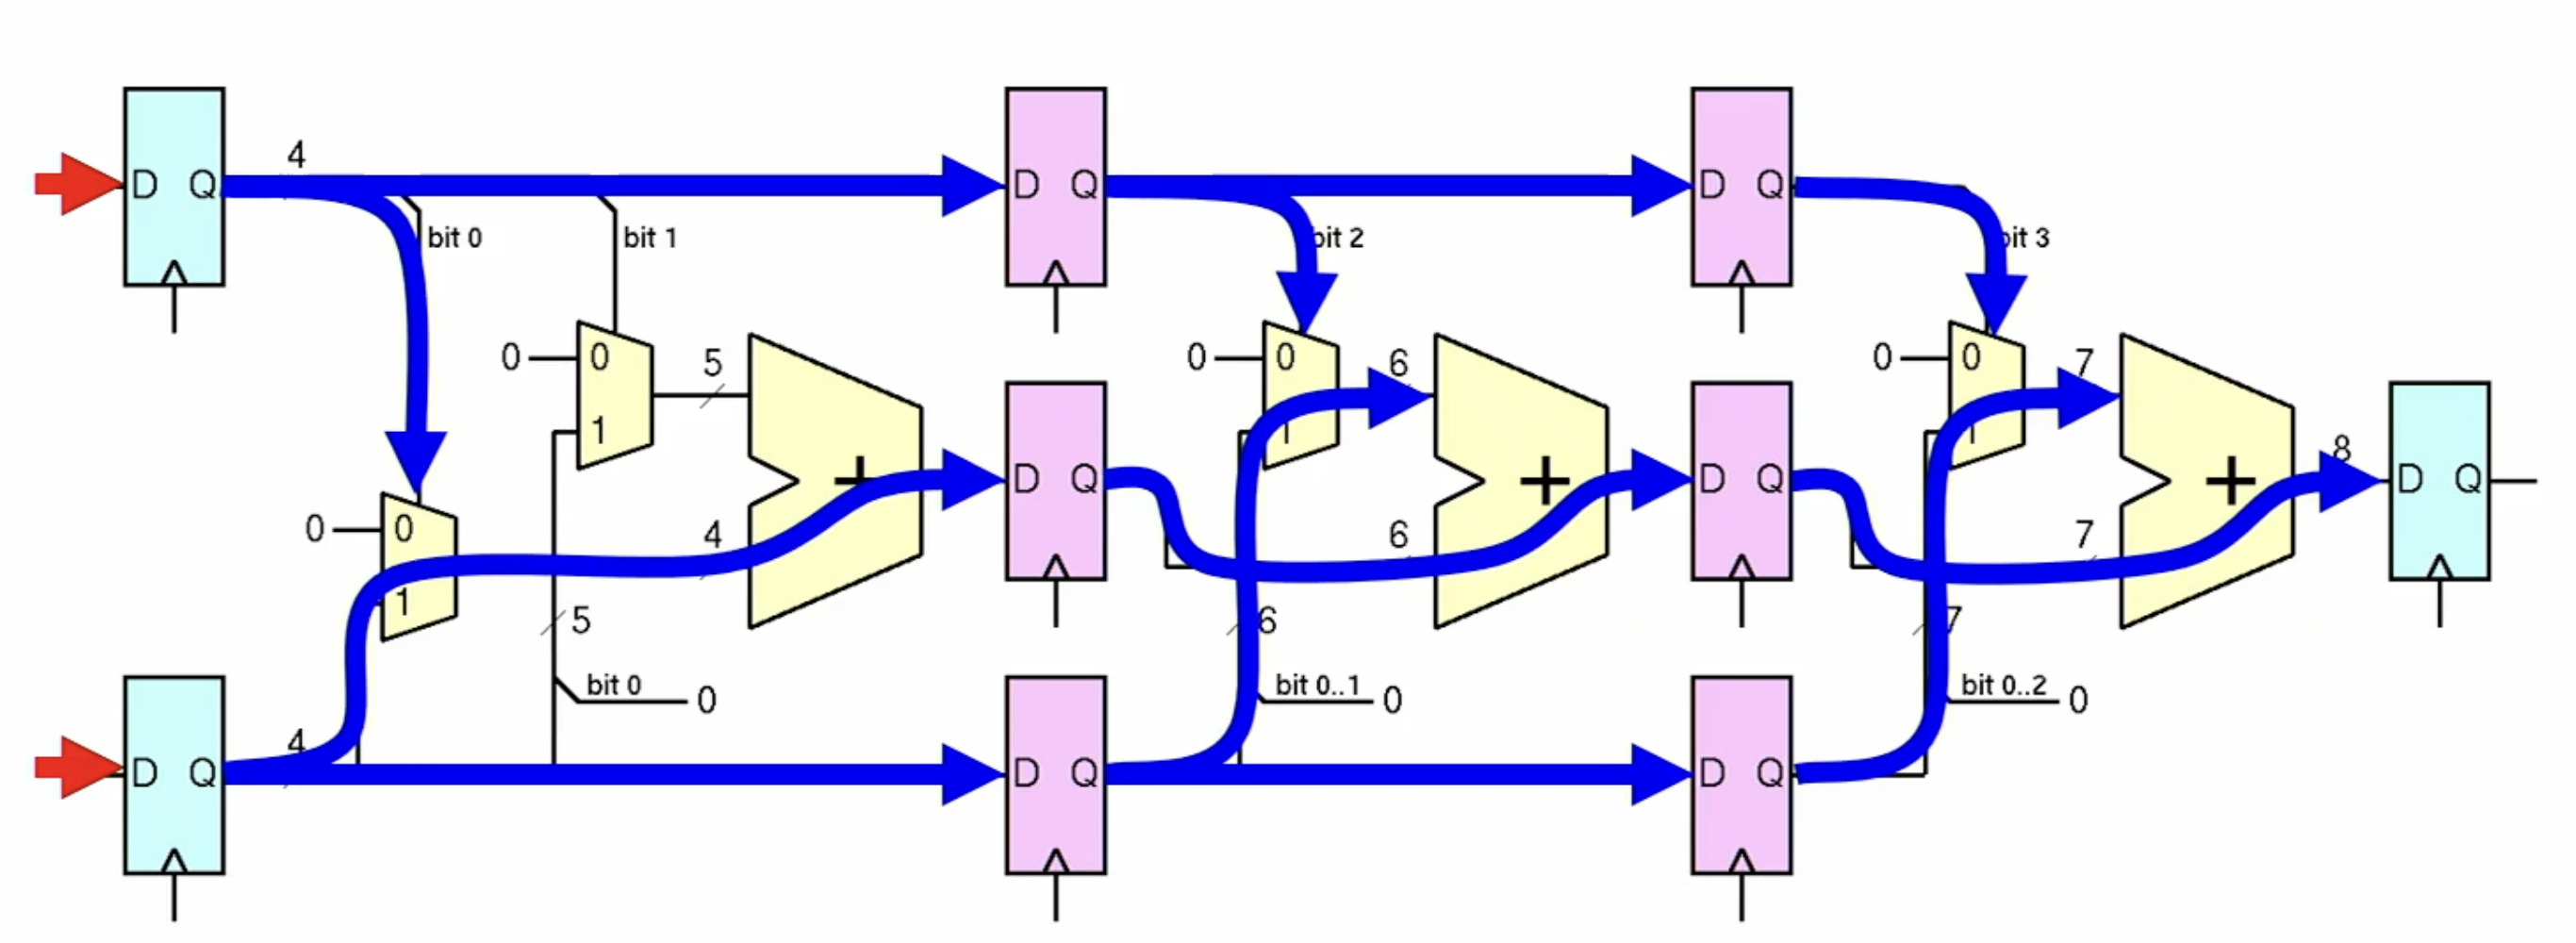
\includegraphics[width=0.65\textwidth]{chapters/chapter4b/images/prop_pipe.png}
\end{center}
\textit{Here for example, we've divided our overall critical path into three smaller segments such that, on the first clock edge, the first segment is processed, and on the second clock edge, the second segment is processed, and so on.}
Now, this new circuit has a shorter critical path, allowing for a faster clock period.
$$T_{\texttt{clock, pipe}} \geq T_{\texttt{new\_critical\_path}} \approx \frac{T_{\texttt{critical\_path}}}{3}$$
While this makes clock periods shorter, it also increases the number of clock cycles required to complete the operation.

\noindent \textbf{Conclusion} \\
The system's functionality remains unchanged, but the clock can run N times faster due to reduced critical path length from intermediate registers, at the cost of requiring N cycles to compute results. This allows for a finer control over the system.

\subsection{Pipelining: Enhancing System Throughput}

Pipelining is a technique widely used in computer architecture to improve the throughput of a system by overlapping the execution of multiple operations. It achieves this by dividing a task into smaller stages, where each stage performs a portion of the overall operation. These stages are connected in a pipeline structure, allowing multiple operations to be processed simultaneously.

\subsubsection*{How Pipelining Works}
A pipeline is divided into distinct stages, each designed to execute a specific part of the operation. For example, in an arithmetic operation, the stages might include fetching data, decoding instructions, performing calculations, and writing results. Each stage operates independently and processes data sequentially.

To understand this, consider a factory analogy where a product goes through three steps:
\begin{itemize}
    \item[] \textbf{Step 1:} Assembly
    \item[] \textbf{Step 2:} Painting
    \item[] \textbf{Step 3:} Packaging
\end{itemize}

In a \textbf{non-pipelined factory}, one worker completes all three steps for one product before starting the next. If each step takes 1 minute, three products would require \( 3 \times 3 = 9 \) minutes.

\hspace{-10px}
\begin{center}
    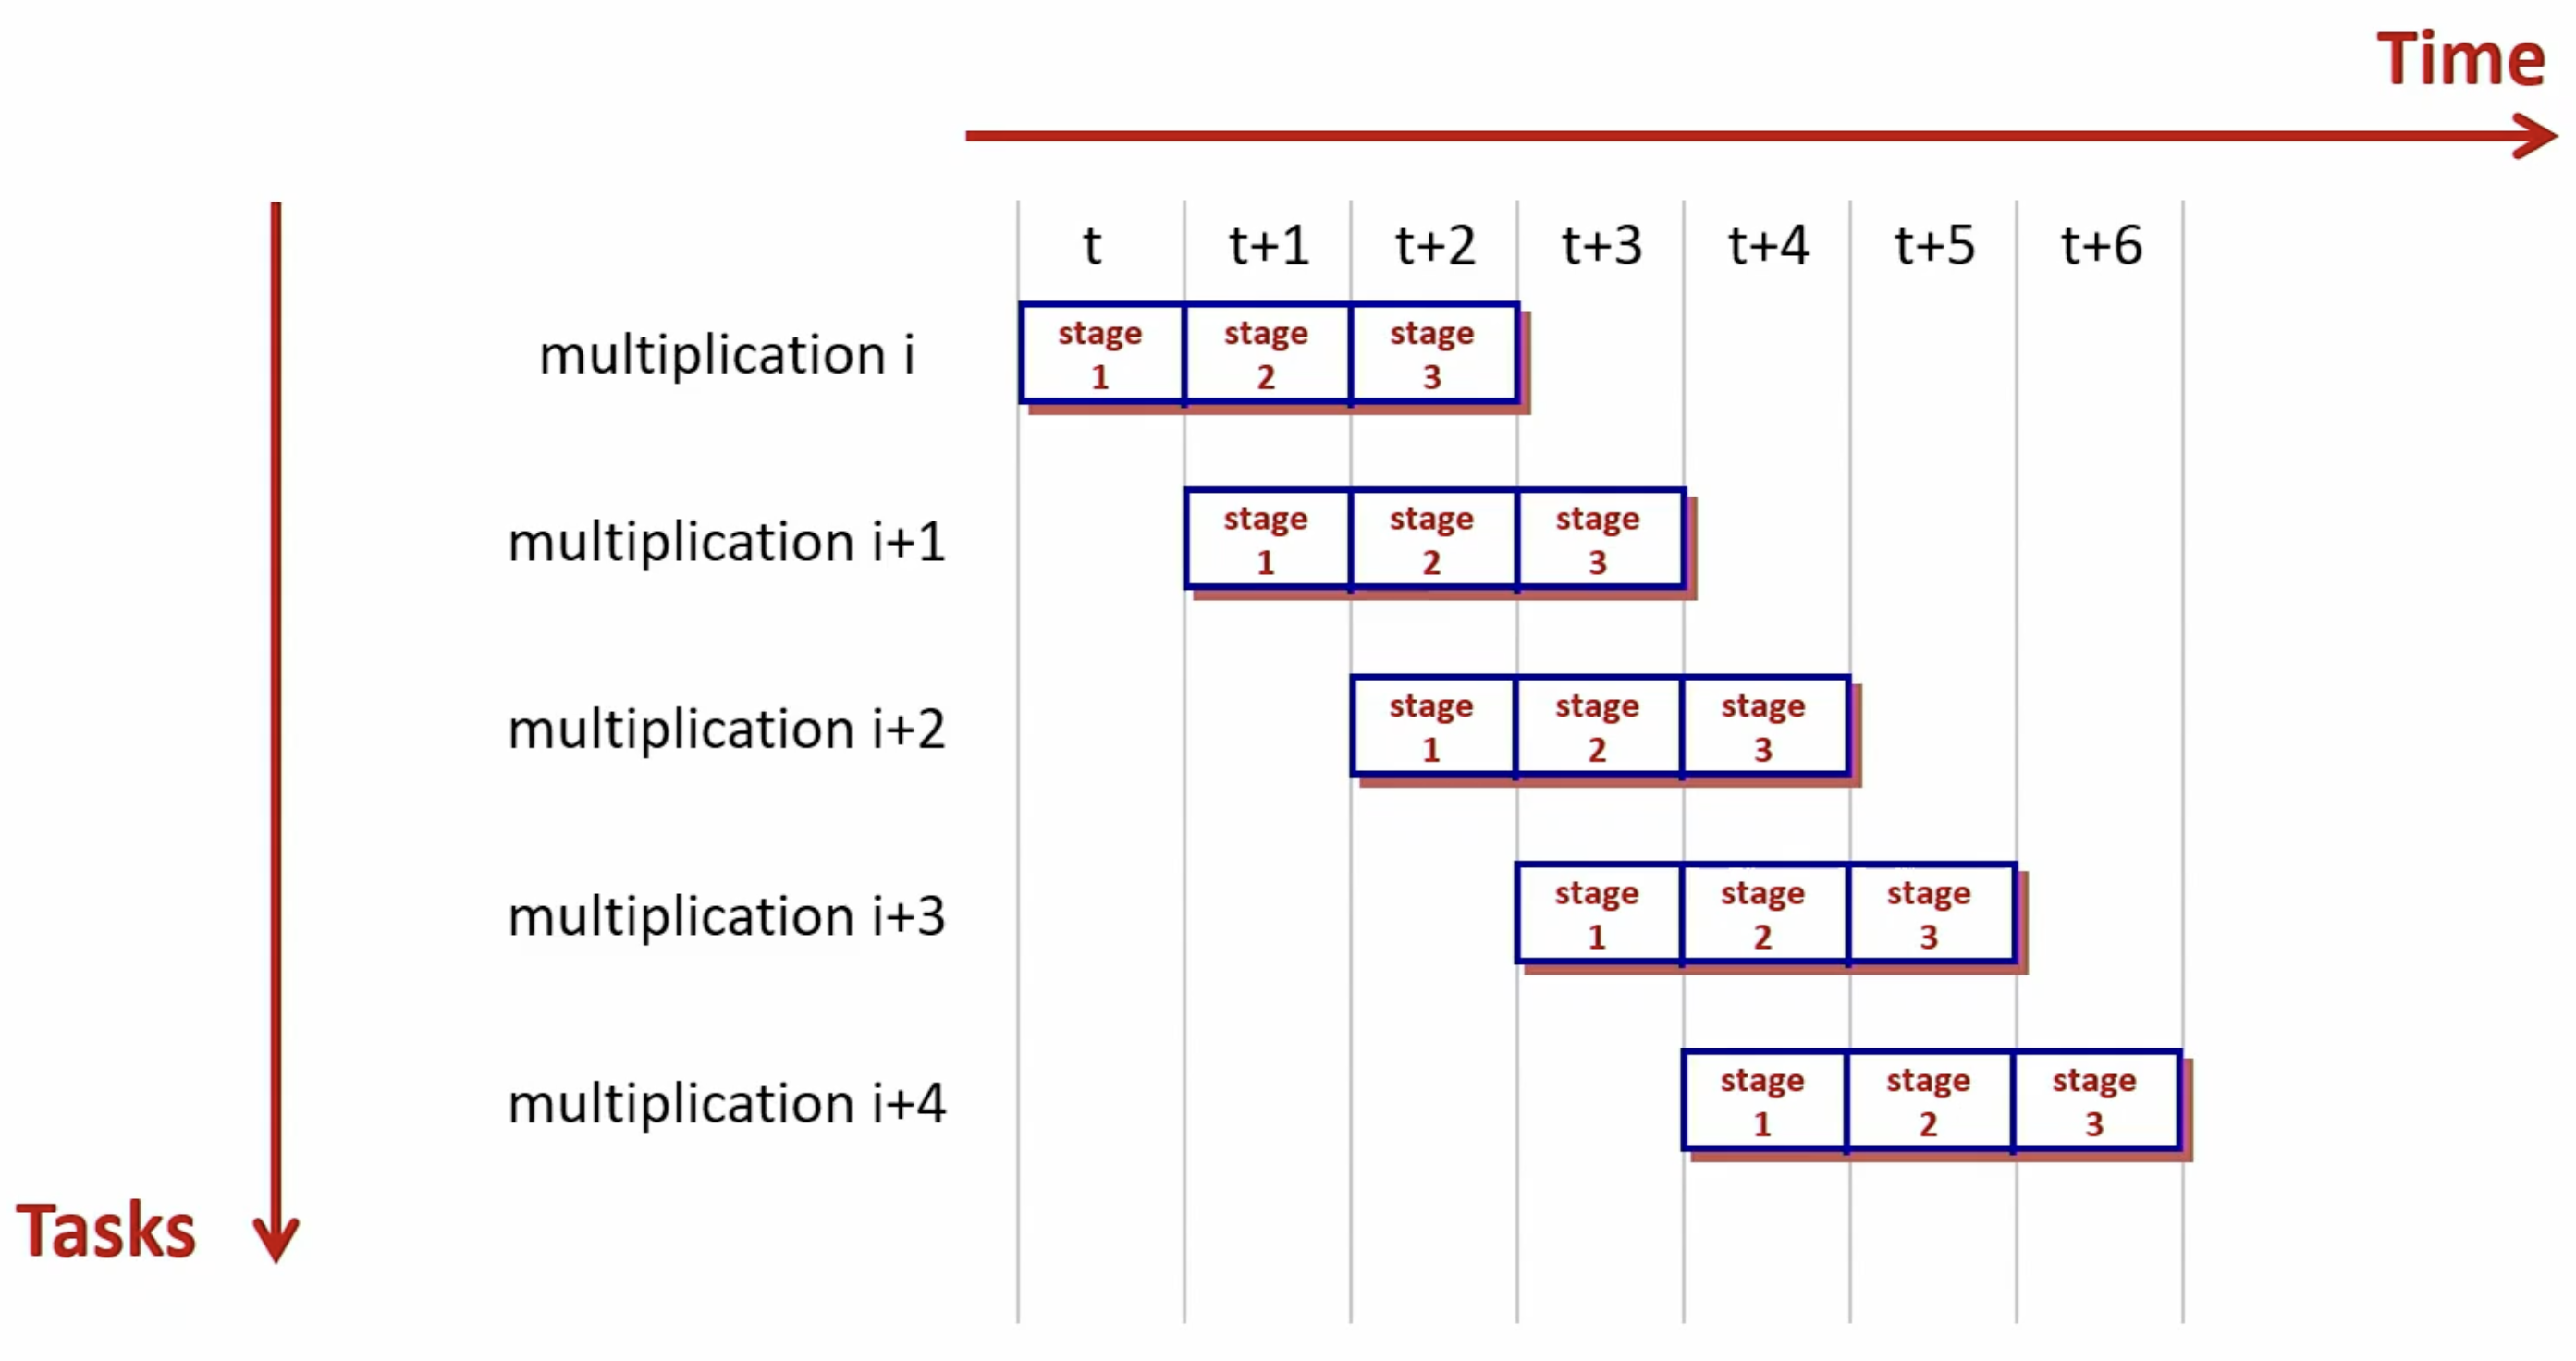
\includegraphics[width=0.65\textwidth]{chapters/chapter4b/images/parallel.png}
\end{center}
In a \textbf{pipelined factory}, the work is divided among three workers:
\begin{itemize}
    \item[] \textbf{At minute 1}, Worker A starts assembling the first product.
    \item[] \textbf{At minute 2}, Worker A starts assembling the second product, while Worker B paints the first.
    \item[] \textbf{At minute 3}, Worker A starts assembling the third product, Worker B paints the second, and Worker C packages the first.
\end{itemize}
By minute 5, all three products are completed, and the pipeline produces one product per minute after it is full.

This overlapping of tasks ensures that all workers are continuously busy, reducing the overall time required to produce multiple products.

\subsubsection*{Advantages of Pipelining}
The key benefits of pipelining include:
\begin{itemize}
    \item[-] \textbf{Improved Throughput:} By overlapping tasks, the system produces results at a faster rate. For instance, once the pipeline is full, one result can be produced per cycle.
    \item[-] \textbf{Efficient Resource Utilization:} Each stage works concurrently on different parts of separate operations, preventing idle resources.
    \item[-] \textbf{Scalability:} Pipelining can accommodate larger workloads by increasing the number of stages, enabling more operations to be processed simultaneously.
\end{itemize}

\subsection{Latency and Throughput}
\noindent \textbf{Latency} \\
Latency refers to the time between the start of a computation and when the result becomes available. It is given by:
\begin{itemize}
    \item \textbf{Original Circuit:} \( T \)
    \item \textbf{Pipelined Circuit:} \( \frac{T}{N} \times N = T \)
\end{itemize}

\noindent \textbf{Throughput} \\
Throughput represents the number of results produced per unit time. It is defined as:
\begin{itemize}
    \item \textbf{Original Circuit:} \( \frac{1}{T} = f \)
    \item \textbf{Pipelined Circuit:} \( \frac{1}{T/N} = \frac{N}{T} = N \times f \)
\end{itemize}

\subsection{Practical Pipelining: Latency and Throughput}
\subsubsection*{Stages and Timing in Pipelining}
Consider a pipeline with $N$ stages, where each stage $i$ takes a time $T_i$ to complete. The pipeline is divided by registers (denoted by red dashed lines), which ensure data is synchronized between stages.
\begin{center}
    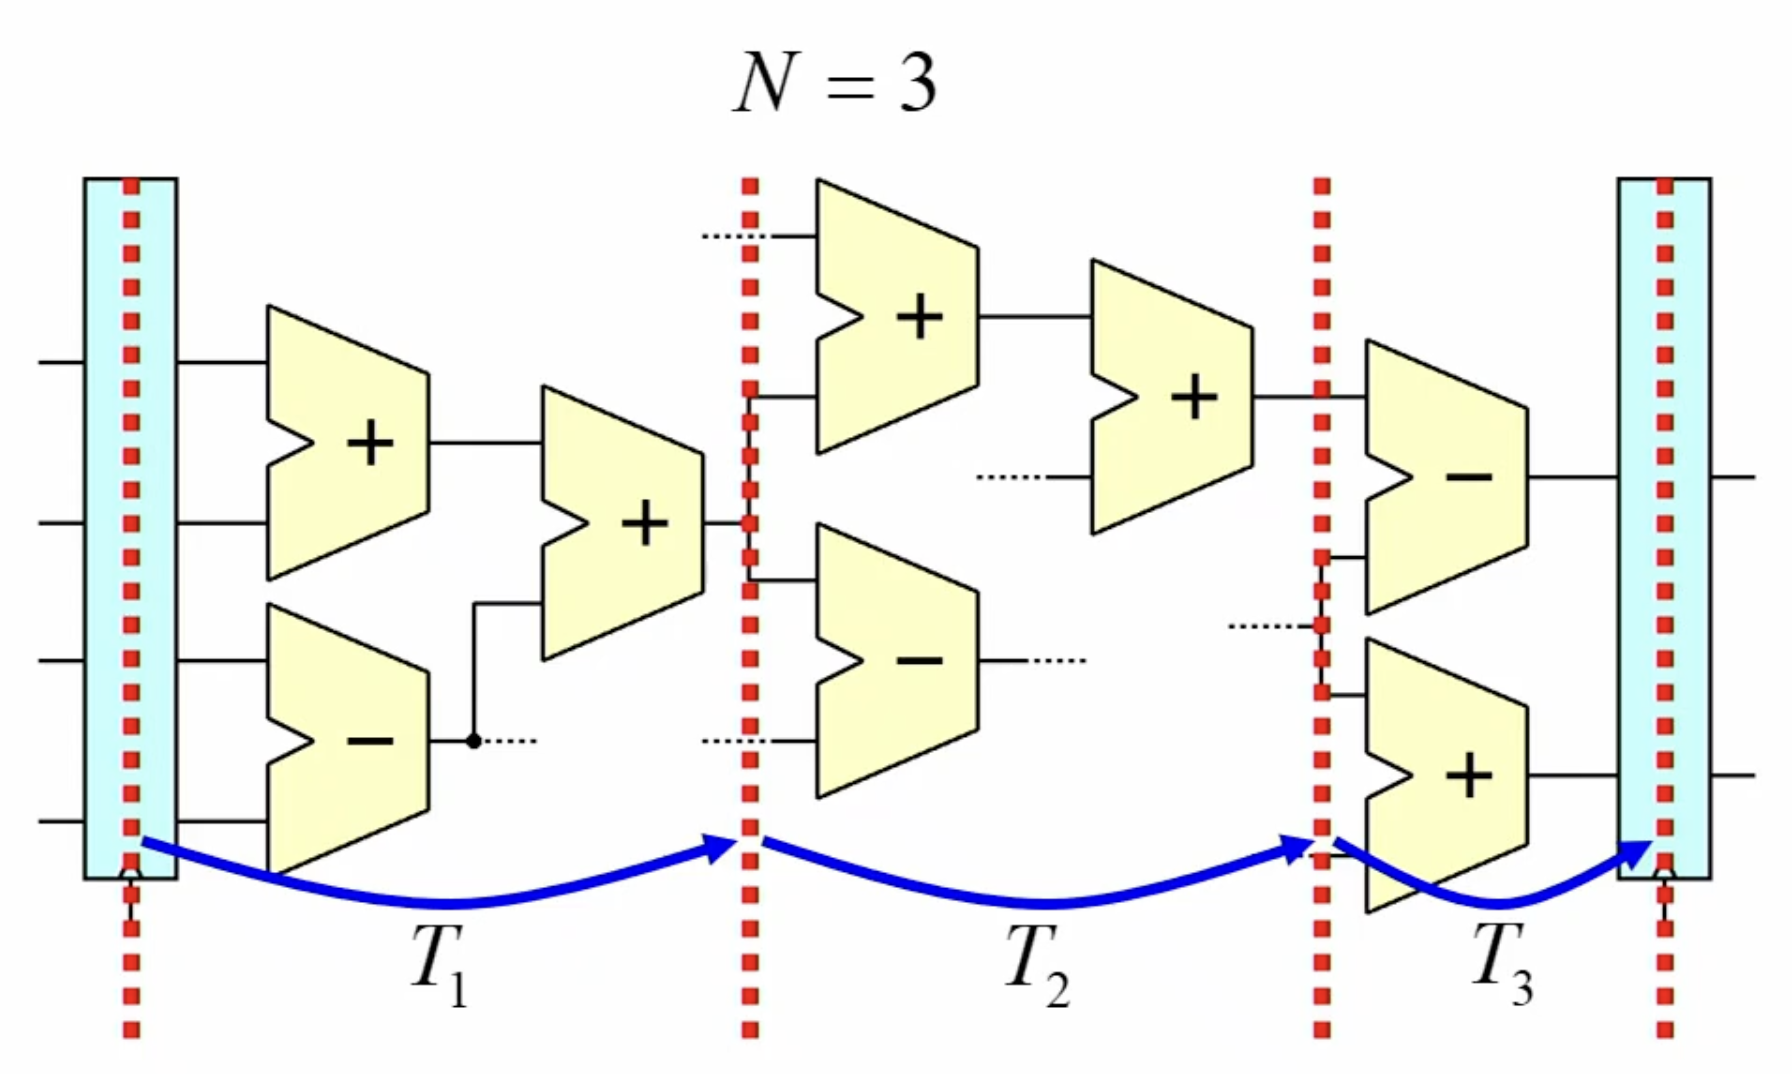
\includegraphics[width=0.45\textwidth]{chapters/chapter4b/images/practical.png}
\end{center}
The overall operation of the pipeline is governed by:
\begin{itemize}
    \item[-] \textbf{Clock Period ($T_\text{CLK,pipe}$):} This is determined by the slowest stage, $T_\text{CLK,pipe} = \max(T_i + T_\text{FF})$, where $T_\text{FF}$ accounts for flip-flop delays.
    \item[-] \textbf{Stage Timing:} Ideally, $T_i \approx T_\text{CLK,comb}/N$, where $T_\text{CLK,comb}$ is the clock period of the original non-pipelined design.
\end{itemize}

\subsubsection*{Latency and Throughput of a Pipeline}

\begin{itemize}
    \item[-] \textbf{Latency ($\lambda_\text{pipe}$):} The latency is the total time required for a single input to propagate through all $N$ stages of the pipeline. It is given by:
    \[
    \lambda_\text{pipe} = N \cdot \max(T_i + T_\text{FF}) = N \cdot T_\text{CLK,pipe}
    \]
    While pipelining increases latency compared to a non-pipelined system, the trade-off is improved throughput.

    \item[-] \textbf{Throughput ($\phi_\text{pipe}$):} Throughput measures how many operations the pipeline can complete in a given time. Once the pipeline is filled, results are produced every clock cycle. It is calculated as:
    \[
    \phi_\text{pipe} = \frac{1}{\max(T_i + T_\text{FF})} = f_\text{pipe}
    \]
    where $f_\text{pipe}$ is the pipeline operating frequency.
\end{itemize}

Pipelining is a practical approach to achieving high-speed operation in digital systems, particularly in processors and signal processing applications. By carefully designing stage timing and managing trade-offs, pipelining can achieve an optimal balance between latency and throughput.
 % Including chapter0.tex from chapters folder
\chapter{Part 4c. Instruction Level Parallelism}
In the last chapter, we've seen how pipelining can make it easier to parallelize indepent operations making it the overall process faster.

\subsection{Pipelining the Processor}
Pipelining in processors is a technique that splits the execution of an instruction into multiple stages, each handled in parallel by separate hardware units. By doing so, multiple instructions can be processed simultaneously, thereby increasing the overall throughput of the processor without increasing the clock frequency.

\begin{itemize}
    \item[-] \textbf{Fetch (F)}: Retrieve the instruction from memory (often from the instruction cache).
    \item[-] \textbf{Decode (D)}: Interpret the fetched instruction, identify operands, and configure the control signals for execution.
    \item[-] \textbf{Execute (E)}: Perform the required operations (e.g., arithmetic, logic, load, store).
\end{itemize}

\noindent In a basic pipeline with three stages (F, D, E), each stage takes one clock cycle. While one instruction is being executed, a second instruction can be decoded, and a third can be fetched at the same time. This overlapping of tasks leads to a substantial improvement in instruction throughput.

\subsubsection*{Example Pipeline Schedule}
Consider a schedule where three instructions (\(i\), \(i+1\), and \(i+2\)) enter the pipeline. Each instruction occupies a unique pipeline stage in any given clock cycle. Figure~\ref{fig:pipeline-schedule} illustrates how each instruction advances one stage every cycle:
\[
\begin{array}{c|cccccc}
\text{Time} & t & t+1 & t+2 & t+3 & t+4 & t+5 \\ \hline
i     & F & D & E & - & - & - \\
i+1   & - & F & D & E & - & - \\
i+2   & - & - & F & D & E & - \\
\end{array}
\]

\subsubsection*{Multi-Cycle Processor vs.\ Pipelined Processor}
A \emph{multi-cycle} processor might use multiple cycles to execute every instruction (e.g., separate cycles for Fetch, Decode, ALU, Memory Access, and Write Back), but only one instruction flows through the processor at a time. In contrast, a \emph{pipelined} processor allows the next instruction to begin its Fetch stage in parallel with the Decode stage of the previous instruction, greatly improving throughput.
\begin{center}
    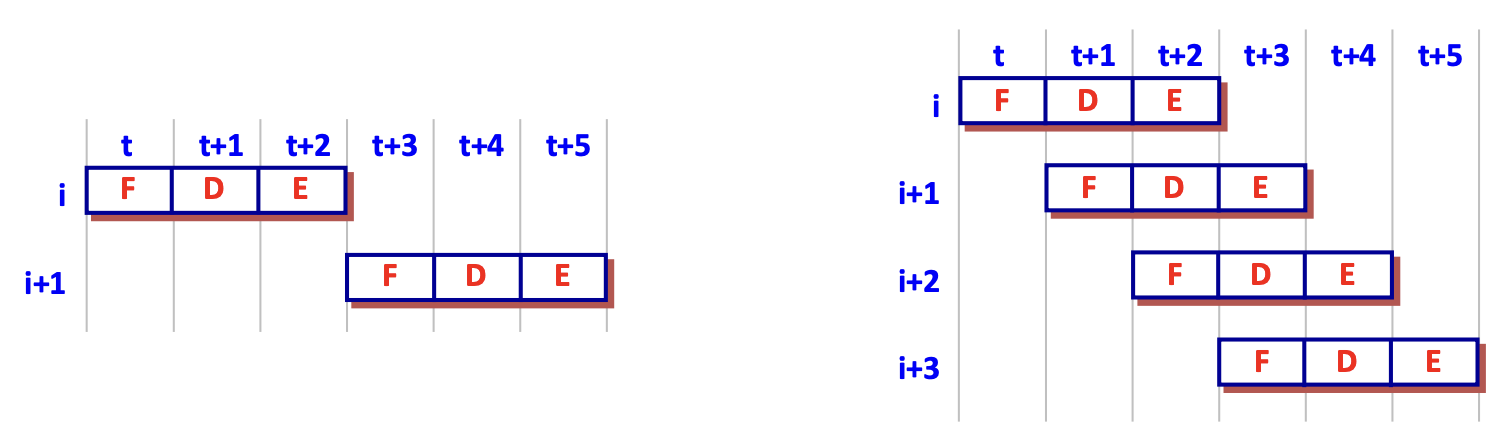
\includegraphics[width=0.65\textwidth]{chapters/chapter4c/images/vs.png}
\end{center}
\subsubsection*{Key Observations for Pipelining}
\begin{enumerate}
    \item \textbf{Repetitive Activity}: Pipelining is effective only when the processor has a large number of instructions to execute.
    \item \textbf{Subactivities}: Each major task (Fetch, Decode, Execute, etc.) should be clearly separable into sub-stages to allow parallel operation.
    \item \textbf{Throughput Gain}: Once the pipeline is full, an instruction completes at the end of every cycle (in the ideal case), increasing throughput.
\end{enumerate}

\noindent Properly designing pipeline stages and handling hazards (such as data, control, and structural hazards) ensures that the pipeline delivers high performance without correctness issues.

\section{Hardware Reuse Across Processor Stages}

In processor design, the approach to hardware reuse varies significantly between multicycle and pipelined architectures. Understanding these differences is crucial for optimizing performance and resource utilization.

\subsection{Multicycle Processor Architecture}

A multicycle processor divides instruction execution into distinct \textbf{states}, allowing certain hardware components to be shared across these states. This sharing is feasible because the components are not required simultaneously, enabling efficient resource utilization.

\begin{itemize}
    \item \textbf{FETCH} State: Typically involves an \textit{adder} to increment the program counter (PC).
    \item \textbf{EXECUTE} State: Requires an \textit{Arithmetic Logic Unit} (ALU) to perform operations.
\end{itemize}

Since the \textit{adder} and the \textit{ALU} are not active concurrently, the ALU can be repurposed to increment the PC during the FETCH state. This reuse reduces the overall hardware complexity and cost.

\subsection{Pipelined Processor Architecture}

In contrast, a pipelined processor operates with multiple \textbf{stages} that are active simultaneously. Each stage performs a different part of the instruction execution process, necessitating dedicated hardware for each stage to avoid conflicts and ensure seamless parallelism.

\begin{itemize}
    \item All pipeline stages are \textit{active concurrently}, handling different instructions in each stage.
    \item Hardware components cannot be shared across stages since multiple instructions require access to the same resources simultaneously.
    \item Consequently, hardware must be \textit{replicated} where necessary to maintain pipeline efficiency and prevent bottlenecks.
\end{itemize}

The inability to share hardware across pipeline stages often leads to increased hardware requirements compared to multicycle processors. However, this replication is essential for achieving high instruction throughput and maximizing pipeline performance.
\newpage
\section{Two Main Challenges in Processor Design}

Designing efficient processors involves addressing several challenges. Two prominent issues are the \textbf{CISC vs. RISC} debate and \textbf{instruction independence}.

\subsection{CISC vs. RISC}
\begin{enumerate}
    \item \textbf{Pipeline Efficiency in CISC vs. RISC}
    \begin{itemize}
        \item[] \textbf{Question}: Can we construct a pipeline for a Complex Instruction Set Computer (CISC) that matches the efficiency of a pipeline designed for a Reduced Instruction Set Computer (RISC)?
        \item[] \textbf{Implications}:
        \begin{itemize}
            \item RISC architectures typically use simpler, fixed-length instructions, which are easier to pipeline efficiently.
            \item CISC architectures have more complex, variable-length instructions, potentially complicating pipeline design and reducing efficiency.
            \item The distinction influences processor complexity, performance, and power consumption.
        \end{itemize}
    \end{itemize}
    \item \textbf{Ensuring Correct Execution with Dependent Instructions}
    \begin{itemize}
        \item \textbf{Issue}: Instructions are often \textit{dependent} on the results of preceding instructions, violating the assumption of \textbf{instruction independence}.
        \item \textbf{Challenge}: Executing code correctly in the presence of such dependencies requires soxphisticated mechanisms to handle hazards, such as data forwarding or pipeline stalls.
    \end{itemize}
\end{enumerate}

Addressing instruction dependencies is critical for maintaining the integrity of program execution while striving for optimal pipeline performance. Techniques such as out-of-order execution and speculative execution are often employed to mitigate the impact of these dependencies.
\section{Multi-Cycle Execution Using an FSM}
In a multi-cycle processor design, each instruction's execution is broken down into multiple steps (states), and the processor transitions through these steps via an FSM.

\subsection{FSM vs.\ Pipeline}
While a pipeline has a fixed sequence of stages (fetch, decode, execute, memory, writeback) for any instruction, an FSM-based multi-cycle design can assign different numbers of steps to each instruction. The FSM transitions vary based on the instruction being executed.



\subsection{Adding Instructions in a Multi-Cycle Design}
When introducing new instructions (e.g., \texttt{lw} or \texttt{add}), the FSM must be extended to accommodate additional states. For example, \texttt{lw} requires computing the address and accessing memory, whereas \texttt{add} mainly requires using the ALU to perform arithmetic. \\
\begin{minipage}[t]{0.45\textwidth}
\textbf{Adding \texttt{add} instruction}\\
We can support the \texttt{add} operation without changing drastically the design, we just need to add it to the ALU.
\[
\text{Fetch} \; \rightarrow \; \text{Decode} \; \rightarrow \; \text{Execute} \; \rightarrow \; \text{Writeback}.
\]
\end{minipage}
\hfill
\vline
\hfill
\begin{minipage}[t]{0.45\textwidth}
\textbf{Adding \texttt{lw} instruction}\\
However, for supporting \texttt{lw} instruction, we need to introduce \textbf{memory} to our design, so we add new steps.
\[
\text{Fetch} \; \rightarrow \; \text{Decode} \; \rightarrow \; \text{Execute} \; \rightarrow \; \text{Memory} \; \rightarrow \; \text{Writeback}.
\]
\end{minipage}
\newpage

\subsection{Adding Instructions to a Pipelined Processor}
Let's look at how this looks like in a pipelined processor.\\
\textit{In this example, we suppose xor and add instructions are both well supported.}
\begin{center}
    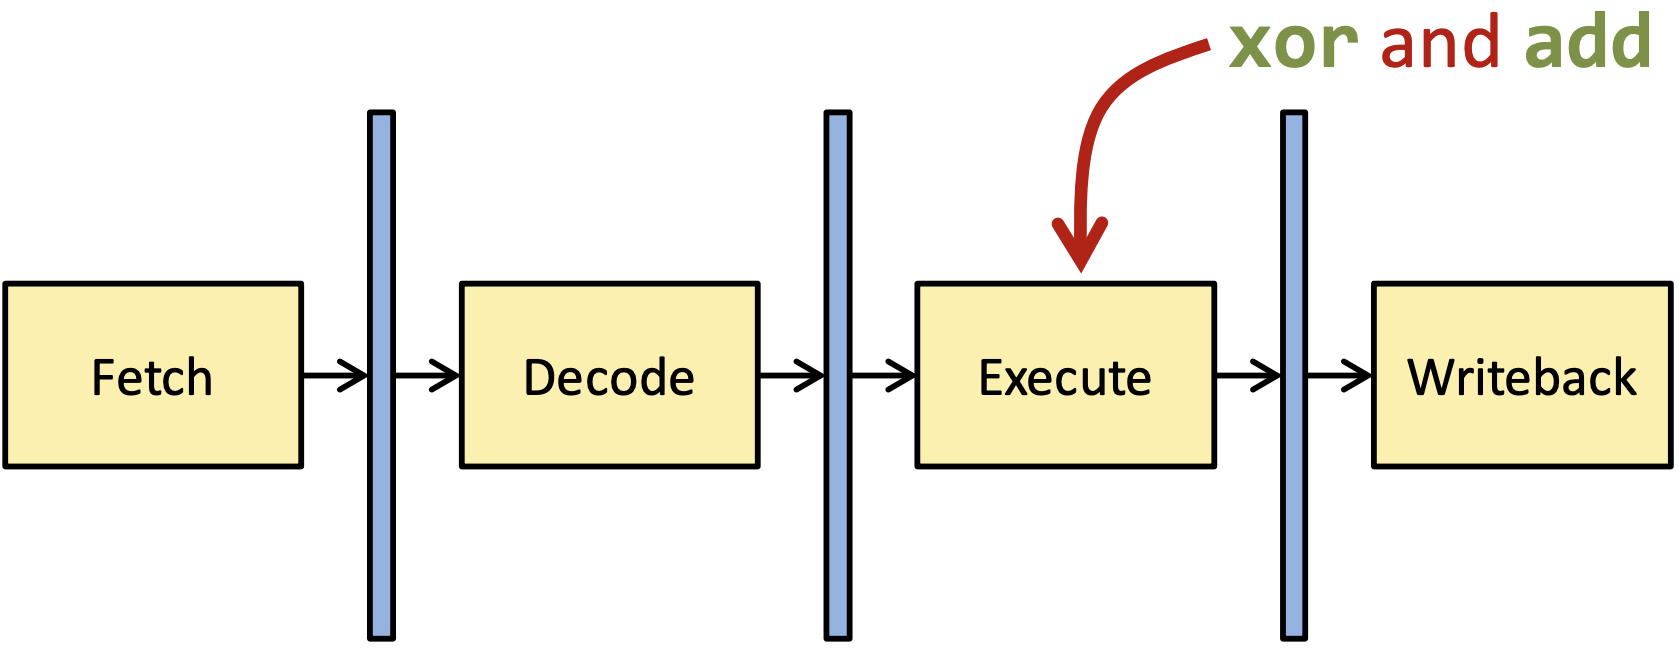
\includegraphics[width=0.45\textwidth]{chapters/chapter4c/images/pipelined-proc.png}
\end{center}
Now, to support \texttt{lw} instruction, we need to add a memory steps, the problem here is that, in a pipelined processor, changes affect \textbf{all instructions}, meaning that now, an \texttt{add} instruction will also take 5 cycles to complete. Thus,
\begin{center}
    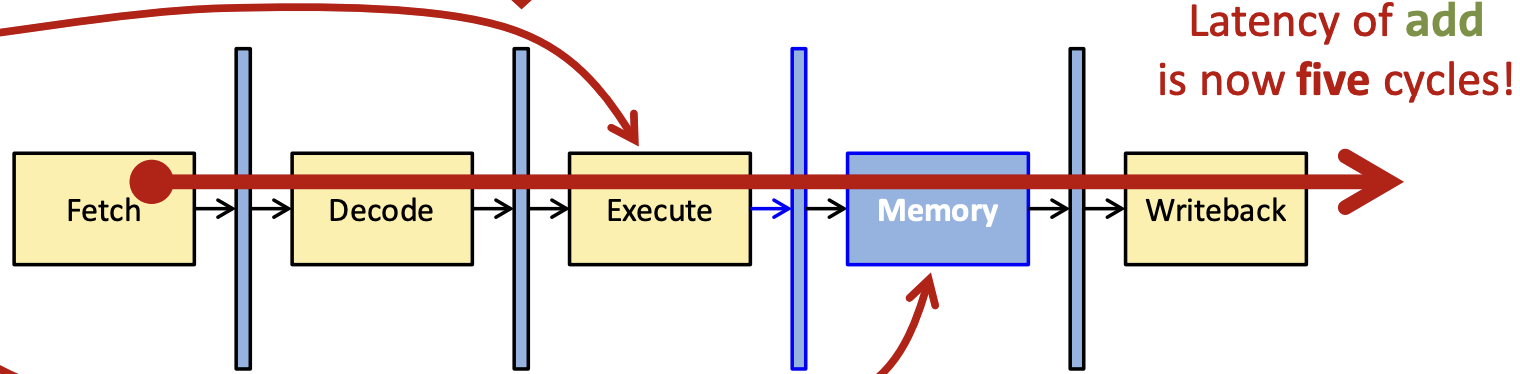
\includegraphics[width=0.45\textwidth]{chapters/chapter4c/images/pipelined-proc-lw.png}
\end{center}

\section{The Importance of the ISA (CISC vs.\ RISC)}
The Instruction Set Architecture (ISA) heavily influences how instructions map onto hardware. A single complex CISC instruction might perform multiple memory accesses and arithmetic operations. In contrast, a RISC instruction set typically emphasizes simplicity: each instruction performs a smaller, more uniform set of operations.

\subsection{A CISC Example}
Consider a hypothetical CISC instruction:
\[
\texttt{sub 8(t4), 0(t1), 0(t2)}
\]
This single instruction might:
\begin{enumerate}
    \item Read the value in memory at address \(\texttt{t2 + 0}\).
    \item Read another value in memory at address \(\texttt{t1 + 0}\).
    \item Subtract these two values.
    \item Finally, store the result in memory at address \(\texttt{t4 + 8}\).
\end{enumerate}
Such complexity can inflate pipeline latency for \emph{all} instructions if the pipeline must accommodate these multi-step operations within a single instruction.
\begin{center}
    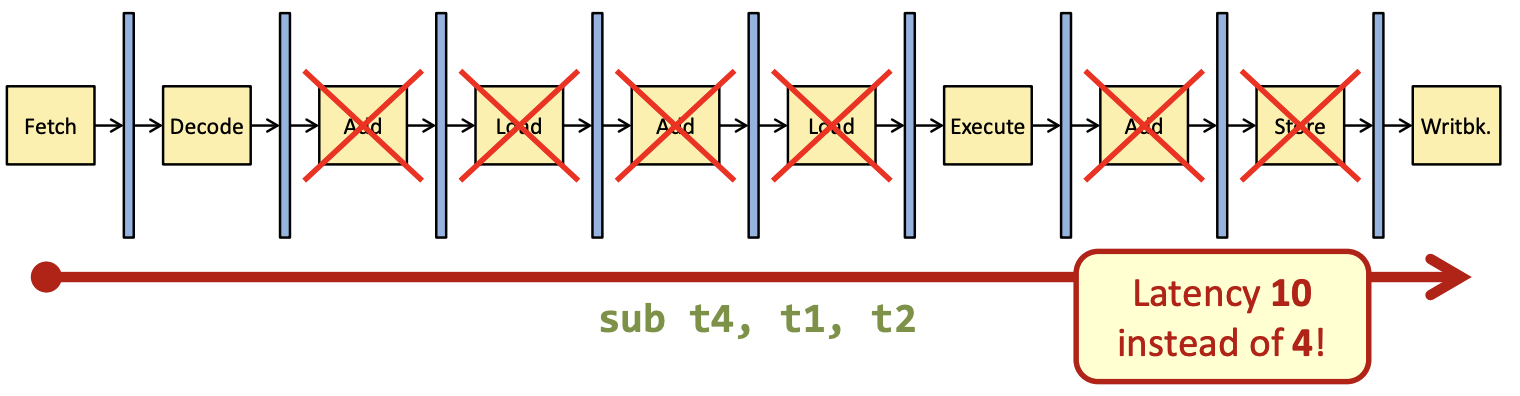
\includegraphics[width=0.65\textwidth]{chapters/chapter4c/images/cisc.png}
\end{center}
\subsection{The RISC Alternative}

Instead of imposing a \textbf{huge penalty} to every simple instruction by making complex instructions possible, the RISC approach advocates for \textbf{only using similarly simple instructions} and building programs with these. \\
\begin{minipage}[htp]{0.45\textwidth}
    \begin{center}
        \begin{tabular}{c c c}
        \texttt{sub 8(t4), 0(t1), 0(t2)} & $\longrightarrow$ &
        \begin{minipage}{0.45\linewidth}
        \texttt{lw t3, 0(t1)} \\
        \texttt{lw t5, 0(t2)} \\
        \texttt{sub t3, t3, t5} \\
        \texttt{sw t3, 8(t4)}
        \end{minipage} \\
        \end{tabular}
        \end{center}
\end{minipage}
\hfill
\vline
\hfill
\begin{minipage}[htp]{0.45\textwidth}
    It turns out that while this is not the only approach, \textbf{it is a good one}, and we will follow it in this course. \\
    In practice, modern CPUs blend design philosophies, using pipelining and other advanced techniques while balancing the complexities of their ISAs. A clear understanding of these concepts---from how an FSM handles instruction steps to how a pipeline benefits from simpler instructions---is crucial to mastering processor design.
\end{minipage}

\subsection{MIPS Pipelining Example}

The MIPS architecture uses a 5-stage pipeline to execute instructions. These stages are: Fetch (F), Decode (D), Execute (E), Memory (M), and Writeback (W). Each instruction moves through these stages, enabling the overlapping of instruction execution, which improves performance by allowing multiple instructions to be processed simultaneously.
\begin{center}
    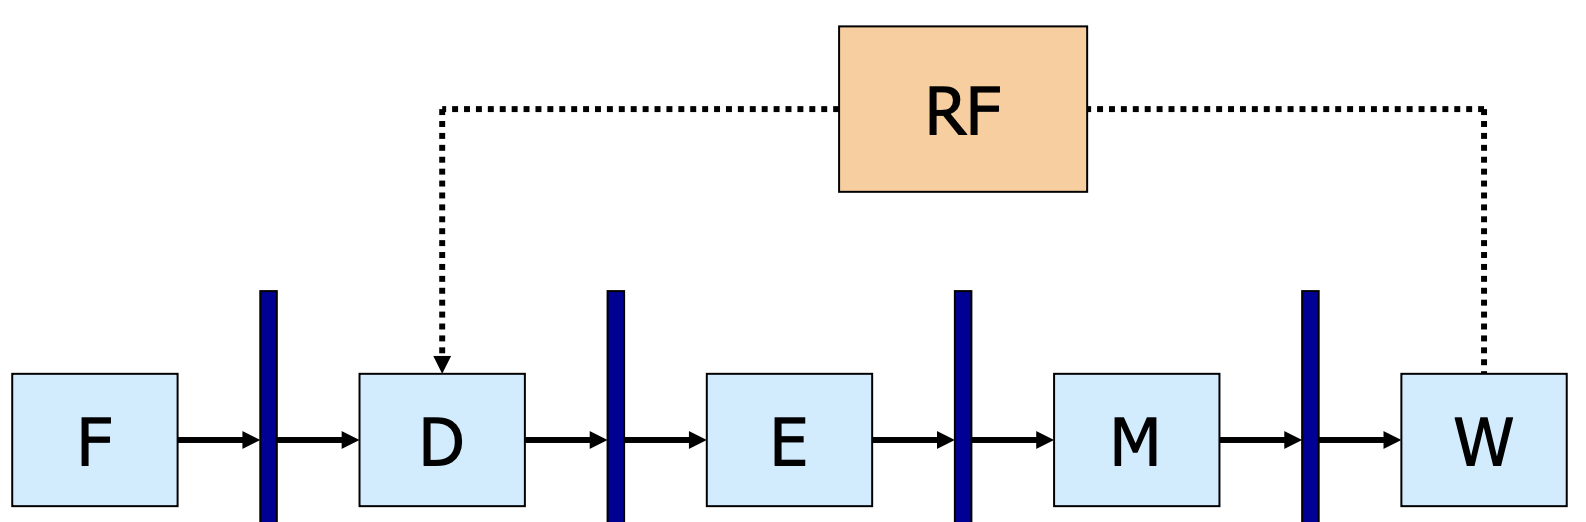
\includegraphics[width=0.45\textwidth]{chapters/chapter4c/images/pipelined-mips.png}
\end{center}
\begin{enumerate}
    \item \textbf{Fetch (F):} The instruction is fetched from the instruction memory.
    \item \textbf{Decode (D):} The instruction is decoded, and the required arguments are obtained from the register file.
    \item \textbf{Execute (E):} The required operation is performed in the Arithmetic Logic Unit (ALU), including address calculations for loads and stores.
    \item \textbf{Memory (M):} Access to data memory is performed if needed, particularly for load and store operations.
    \item \textbf{Writeback (W):} The result of the operation, whether from the ALU or memory, is written back to the register file.
\end{enumerate}

This pipelining model allows instructions to be executed in parallel, thus improving the throughput of the processor and allowing more efficient use of system resources.

\subsection{The Laundry Metaphor for Pipelining}
Pipelining in computer architecture can be explained using the laundry metaphor. Consider the tasks involved in doing laundry: washing, drying, folding, and putting away. Each of these steps represents a stage in the pipeline.
\begin{center}
    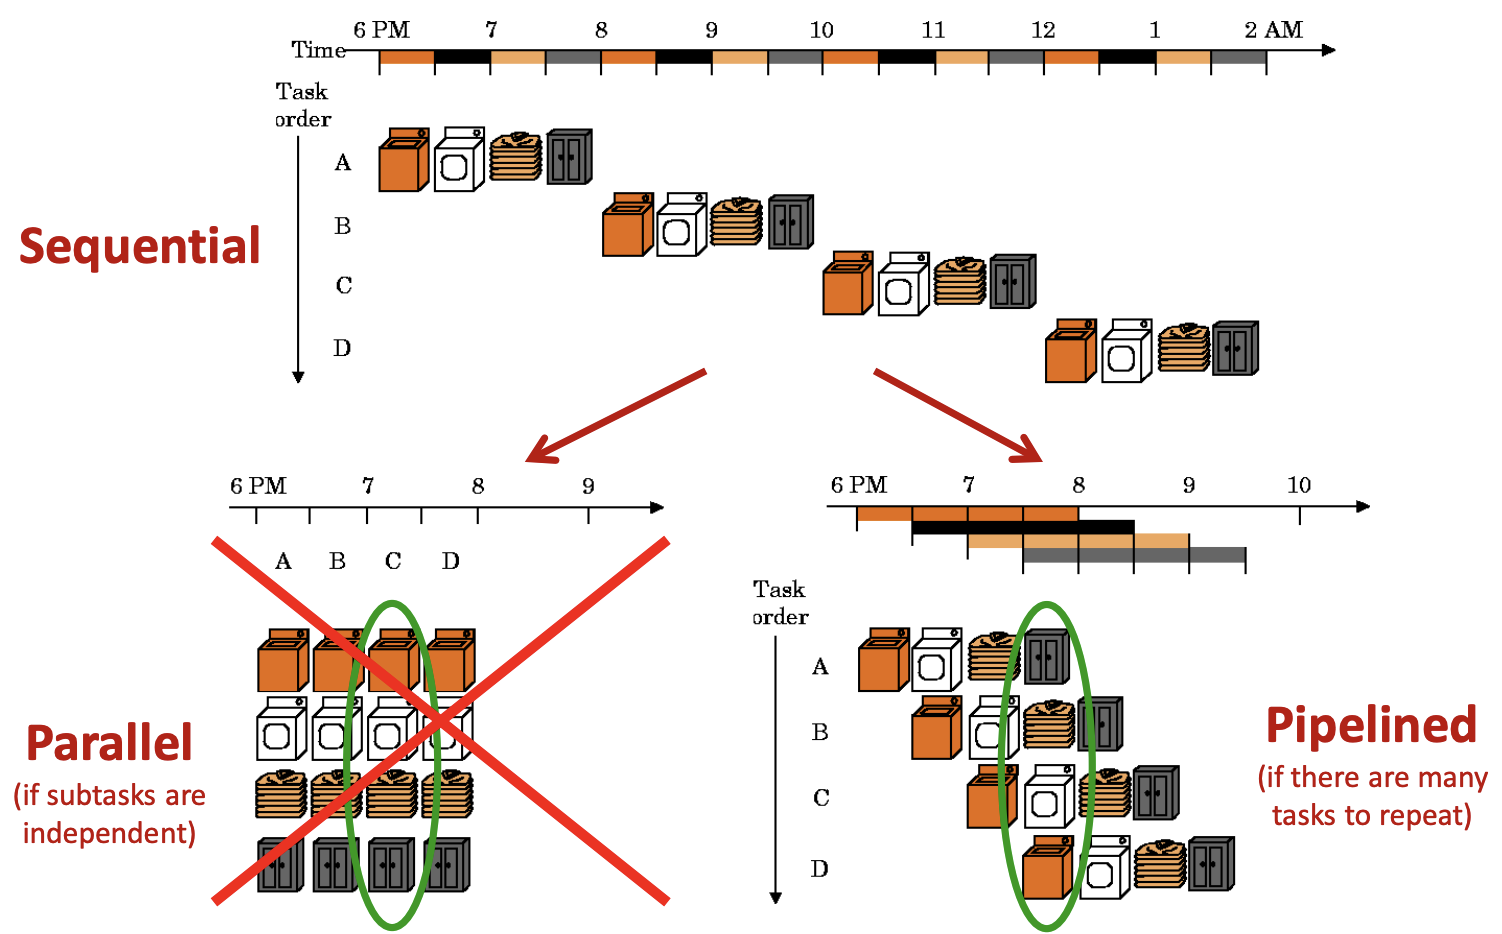
\includegraphics[width=0.65\textwidth]{chapters/chapter4c/images/laundry.png}
\end{center}
\begin{itemize}
    \item[-] \textbf{Sequential Execution:} In a sequential process, one load of laundry is completed through all stages before starting the next. This approach takes a long time because each load must wait for the previous one to finish.
    \item[-] \textbf{Parallel Execution:} If the subtasks are completely independent, multiple washing machines, dryers, and folders could be used simultaneously. However, this is often impractical due to resource limitations.
    \item[-] \textbf{Pipelined Execution:} In pipelining, multiple loads of laundry are processed simultaneously, with each load at a different stage. For example, while one load is being washed, another is dried, and a third is folded. This overlaps the tasks, significantly reducing total time.
\end{itemize}

\newpage
\subsection{Two Distinct Memory Interfaces in MIPS}

In a MIPS processor, two distinct memory interfaces are utilized to enhance performance by allowing concurrent operations: the 	extbf{Instruction Cache} and the 	extbf{Data Cache}. These interfaces are depicted in the following architecture:
\begin{center}
    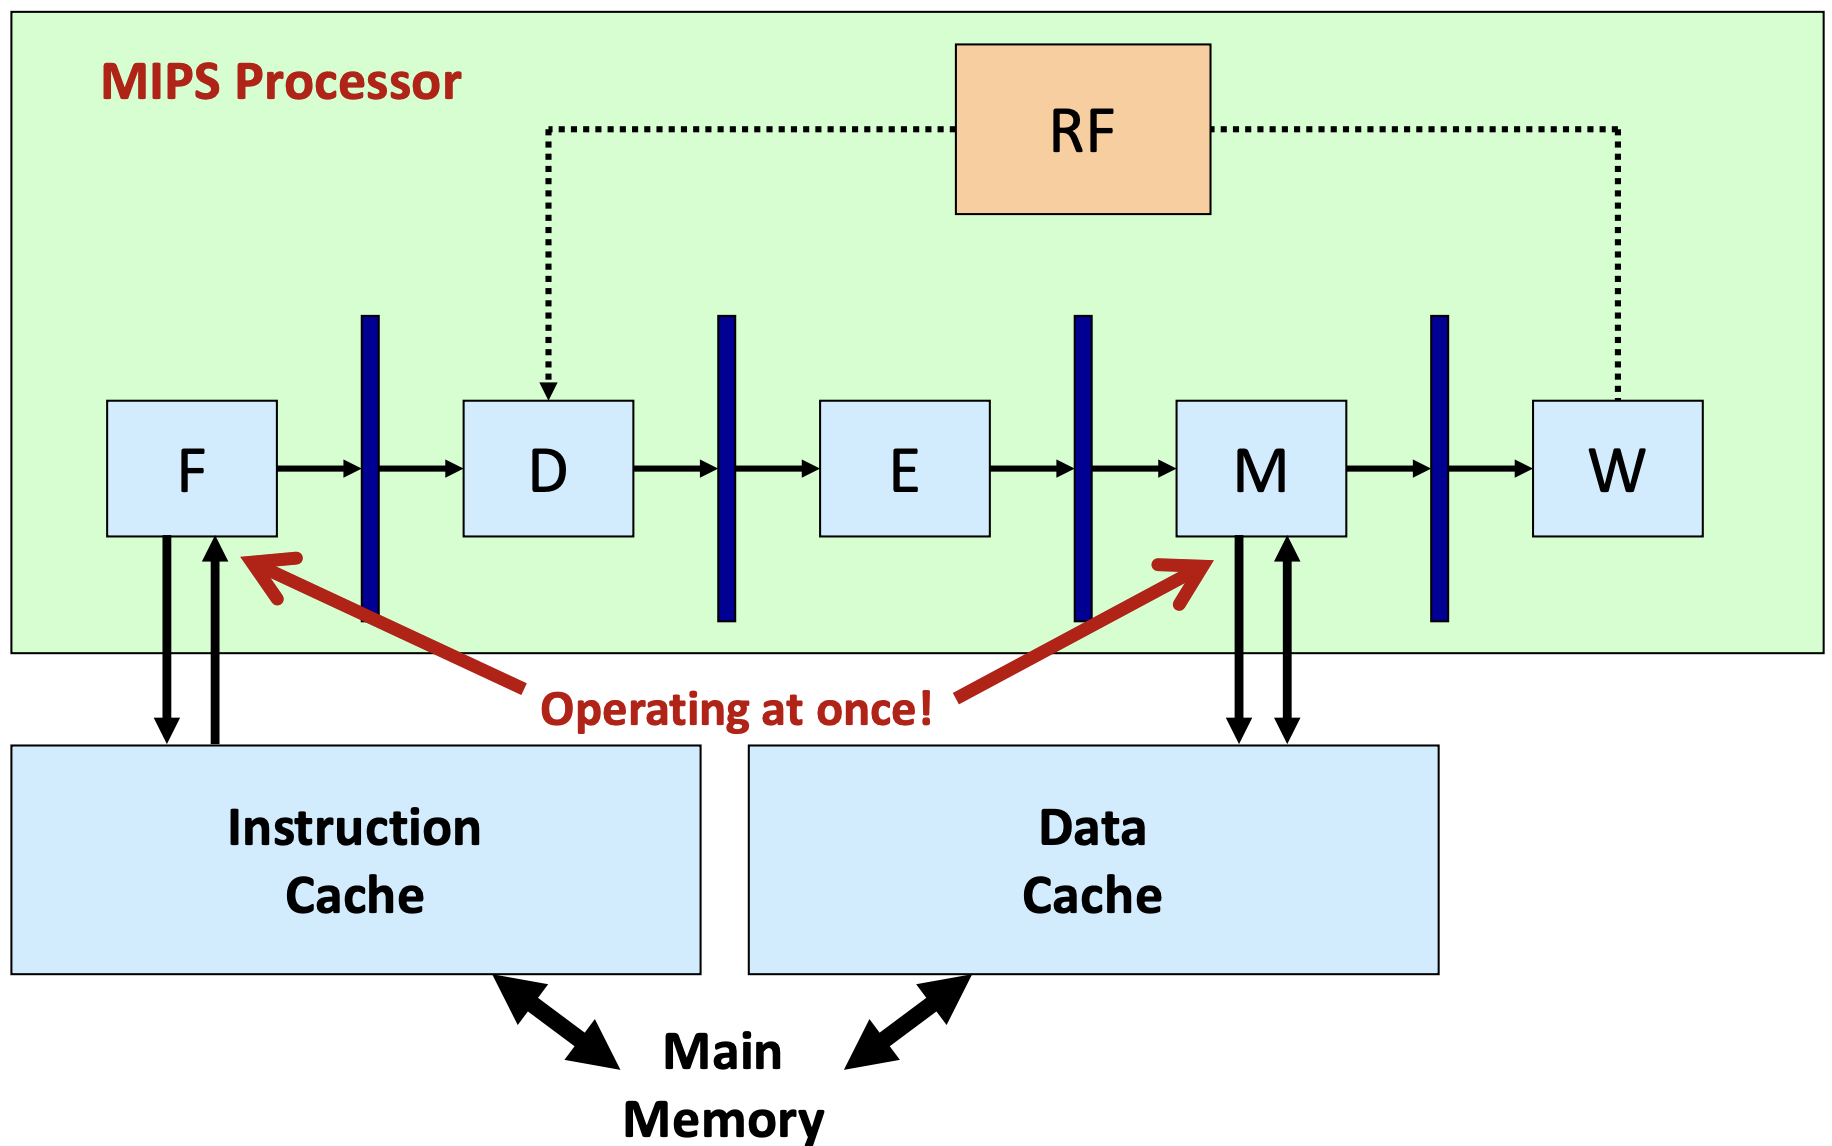
\includegraphics[width=0.45\textwidth]{chapters/chapter4c/images/mips.png}
\end{center}
\begin{itemize}
    \item[-] The \textbf{Instruction Cache} is accessed during the \textbf{Fetch} (F) stage, retrieving instructions for execution.
    \item[-] The \textbf{Data Cache} is utilized during the \textbf{Memory} (M) stage, providing data required for processing.
\end{itemize}

The pipeline stages of the MIPS processor are as follows:
\begin{enumerate}
    \item \textbf{F (Fetch)}: Instructions are fetched from the Instruction Cache.
    \item \textbf{D (Decode)}: Instructions are decoded, and operands are prepared using the Register File (RF).
    \item \textbf{E (Execute)}: The instruction is executed.
    \item \textbf{M (Memory)}: Data is accessed from or written to the Data Cache.
    \item \textbf{W (Write-back)}: Results are written back to the register file.
\end{enumerate}

The separation of memory interfaces allows the Instruction and Data caches to operate simultaneously, enabling improved throughput and reduced bottlenecks in the pipeline. Additionally, the Register File (RF) facilitates data flow between the stages.

This dual-interface approach is critical for high-performance pipelined architectures, allowing overlapping of instruction fetch and memory access operations.

\subsection{Example of Pipelined Execution }
\includemedia[
  width=0.6\linewidth, % Adjust width
  activate=onclick,
  addresource=video.mp4, % Video file
  flashvars={source=chapters/chapter4c/images/video.mp4}
]{}{VPlayer.swf}
 % Including chapter0.tex from chapters folder
\end{document}

